\chapter{Torus embeddings}\label{chap1}

For\pageoriginale simplicity, we work over an algebraically closed
field $k$ of arbitrary characteristic. All $k$-algebras are
commutative with unity and all $k$-algebra homomorphisms preserve
unity. Although rather unconventional, we mean by an algebraic
variety a reduced, irreducible and separated scheme over $k$ which is
only \textit{locally} of finite type, i.e. possibly an infinite union
of open subsets which are usual affine varieties of finite type.  


\section{Algebraic tori}\label{chap1:sec1}%section 1

In this section, we recall basic facts about algebraic tori which we
use later. 

We denote by $k^*$ the multiplicative group of non-zero elements of
$k$ considered as an \textit{algebraic group} over $k$. It is usually
denoted by $G_m$ and is the affine algebraic group Spec$(k[t,t^{-1}])$
endowed with the comultiplication $t\longmapsto t \otimes t $ on the
coordinate ring. It is more convenient to consider it as a group
functor which assigns to a $k$-algebra $B$ its multiplicative group
$B^*$ of  units. 

An \textit{algebraic torus} over $k$ is an algebraic group $T$
isomorphic to a finite direct product $k^* \times \cdots \times k^*$. 

Mutually dual free $\mathbb{Z}$-modules $M$ and $N$ with the pairing
$\langle , \rangle : M \times N \rightarrow \mathbb{Z}$ give rise to
an algebraic torus 
$$
T = \Hom_{gr}(M,k^*) = N \otimes_{\mathbb{Z}} k^*.
$$\pageoriginale
Conversely, an algebraic torus $T$ gives rise to the character group 
$$
M = \Hom_{\text{alg.gr}}(T,k^*)
$$
and the group of 1-parameter subgroups
$$
N = \Hom_{\text{alg.gr}}(k^*,T),
$$
both written additively, together with the duality pairing  
$$
\langle~ , \rangle : M \times N \rightarrow \Hom_{\text{alg.gr}} (k^*,k^*) =
\mathbb{Z}. 
$$

\noindent
For $m$ in $M$, we denote by $e(m) : T \rightarrow k^*$ the
corresponding character. The coordinate ring $\ulcorner (0_T)$ is the
group algebra of $M$ over $k$ with $\{ e(m) ; m \in M\}$ forming a
$k$-basis and with $e(m + m') = e(m) e(m')$. For $n$ in $N$, the
corresponding 1-parameter subgroup sends $t$ in $k^*$ to the element
$t^{\langle ? , n \rangle}$ of $T = \Hom_{gr}(M,k^*)$ which maps $m$
in $M$ to $t^{\langle m,n \rangle}$ in $k^*$. 

A homomorphism $f : T \rightarrow T'$ of algebraic tori correspond in
one-to-one fashion with a homomorphism $f_* : N \rightarrow N'$ and a
homomorphism $f^* : M' \rightarrow M$, where $N'$ and $M'$ are,
respectively, the group of 1-parameter subgroups and character group
of $T'$. The following fact is quite relevant to us later: $f$ is
surjective if and only if $f_*$ has finite cokernel (resp. $f^*$ is
injective). 

The main reason why things work out so well later is that algebraic
tori are the only algebraic groups which, besides being connected and
commutative, satisfy the following basic complete reducibility
property: 

\begin{theorem*}
Every\pageoriginale algebraic representation of an algebraic torus is
completely reducible, and is in fact a direct sum of one dimensional 
representations, i.e. characters. 
\end{theorem*}

For the proof of this theorem as well as other basic facts about
algebraic groups, we refer the reader to Borel \cite{keyB1}. 

\section{Torus embeddings and Summaries theorem}\label{chap1:sec2}

An algebraic action of an algebraic torus $T$ on an algebraic variety
$X$ is a morphism $T \times X \rightarrow X$ satisfying the usual
axioms $(tt')x = t(t'x)$ and $ex = x $ for $t, t' \in T$, $x \in X$
and  $e=$ (the identity of $T$). When algebraic tori $T$ and $T'$ act
on algebraic varieties $X$ and $X'$, respectively, an
\textit{equivariant morphism} consists of a homomorphism $f : T
\rightarrow T'$ and a morphism $\bar{f} : X \rightarrow X'$ such that
$\bar{f}(tx) = f(t) \bar{f} (x)$ for $t \in T$ and $x \in X$. 

Here is one of the basic results about torus actions:

\begin{theorem*}[(Sumihiro)]
If an algebraic torus $T$ acts algebraically on a {\em{normal}}
algebraic variety over $k$ {\em{locally of finite type}}, then $X$ is
covered by T-stable {\em{affine}} open subsets of finite type. 
\end{theorem*}

We do not repeat the proof  here and refer the reader to \cite{keyS3} or
\cite[I.2, Thm.5]{keyTE}. Note that since Pic$(G)$ is finite by
\cite[Cor. VII 1.6]{keyR2}, the argument in \cite{keyTE} can be
modified to cover the general 
case in \cite{keyS3}. Ishida pointed out that if an algebraic group $G$ acts
on $X$ locally of finite type, then $X$ is covered by\pageoriginale
$G$-stable open sets of finite type to which \cite{keyS3} applies. 

\begin{remark*}
As was pointed out by H.Matsumura, the assertion of the theorem is not
true unless $X$ is normal. Indeed, $T = k^*$ acts on the rational
curve $X$ with a node obtained by identifying the zero and the point
at infinity of the projective line $P_1$. The node does not have any
$T$-stable affine open neighborhood. When $k = \mathbb{C},
\mathbb{C}^*$ acts {\em{analytically}} on an elliptic curve $E$,
which is the quotient of $\mathbb{C}^*$ by an infinite cyclic
subgroup. Obviously, there is no $\mathbb{C}^*$-stable open
neighborhood. (cf. \S. \ref{chap2:sec11}). 
\end{remark*}

When an algebraic torus $T$ acts on $X$, not much is lost, even if we
assume the action to be (even scheme-theoretically)
\textit{effective}. Indeed, since $T$ is commutative, we can replace
$T$ by its quotient torus by the kernel of the canonical homomorphism
from $T$ to the automorphism group functor \textit{Aut$(X)$}. In these
notes, we are interested in almost homogeneous (or sometimes called
pre-homogeneous) algebraic torus actions on irreducible algebraic
varieties, i.e. those which have a dense orbit. The dense orbit is
necessarily Zariski open, and is isomorphic to $T$ when the action is
effective. Thus we are led to the following: 

\begin{defi*}
A \textit{torus embedding} $T \subset X$ consists of an algebraic
variety $X$ containing $T$ as a Zariski open dense subset and an
algebraic action of $T$ on $X$ which extends the group law of $T$,
i.e. we have a commutative diagram 
\[
\xymatrix{
T \times X \ar[r] \ar@{}[d]|{\bigcup} & X \ar@{}[d]|{\bigcup}\\ 
T \times T \ar[r] & T.
}
\]

\end{defi*}

\noindent
An\pageoriginale equivariant dominant morphism from a torus embedding
$T \subset X$ to another $T' \subset X'$ is a dominant morphism
(i.e. with dense image) $f : X \rightarrow X'$ whose restriction to
$T$ induces a \textit{surjective} homomorphism $f|T : T \rightarrow
T'$ and which is equivariant with respect to the actions, i.e. the
following diagram is commutative:   
\[
\xymatrix{
T \times X \ar[r] \ar[d]_{(f|T) \times f} & X \ar[d]^f\\
T' \times X' \ar[r] & X'
}
\]

\noindent
Thus we have the category of torus embeddings.

Although dominant morphisms look too restrictive, those are the only
equivariant morphisms which can be described in terms of
r.p.p. decompositions. 

We will give typical examples of torus embeddings in \S. \ref{chap1:sec7}.

\section{Rational partial polyhedral decompositions}\label{chap1:sec3}

We denote by $\mathbb{Z}, \mathbb{Q}$ and $\mathbb{R}$ the set of integers,
rational numbers and real numbers, respectively. $\mathbb{Z}_0,
\mathbb{Q}_0$ and $\mathbb{R}_0$ are the sets of \textit{non-negative} elements
in them, respectively. 

For a free $\mathbb{Z}$-module $N \cong \mathbb{Z}^r$ of rank $r$, let
$M = Hom_{\mathbb{Z}}(N,\mathbb{Z})$ be its dual $\mathbb{Z}$-module
with the canonical pairing $\langle ~, \rangle : M \times N
\rightarrow \mathbb{Z}$. We denote their scalar extensions to $\mathbb{R}$ by
$N_{\mathbb{R}} = \mathbb{R} \otimes_{\mathbb{Z}} N$, $M_{\mathbb{R}}$ and $\langle
~,\rangle : M_{\mathbb{R}} \times N_{\mathbb{R}} \rightarrow \mathbb{R}$. 

\begin{defi*}
A subset $\sigma \subset N_{\mathbb{R}}$ is called a strongly convex rational
polyhedral cone with apex $0$ (or simply a {\em{cone}} later) if
$\sigma \cap (- \sigma) = \{ 0\}$ and there exist $n_1,\ldots, n_s$ in
$N$ such that 
\end{defi*}
$$
\sigma = \mathbb{R}_\circ n_1 +\cdots+\mathbb{R}_\circ n_1= \{\ a_1
n_1 +\cdots + a_s n_s ; a_1 ,\ldots , a_s \in \mathbb{R}_\circ \}. 
$$\pageoriginale
$n_1,\ldots, n_s $, under the condition that they are irrredundant
with each $n_1$ a primitive element of $N$), are uniquely determined
by $\sigma$ and are called the \textit{ fundamental generators } of
$\sigma. \dim \sigma$ is the dimension of the $\mathbb{R}$-vector
subspace $\sigma + ( - \sigma)$ in $N_{\mathbb{R}}$ generated by
$\sigma$.  

	When rank $N =3$, the following are example of cones.  
\begin{figure}[H]
\centering 
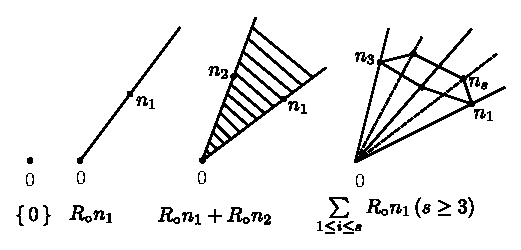
\includegraphics{vol58-fig/fig58-1.eps} 
\end{figure}

\begin{defi*}
Let $\sigma$ be a cone in $N_{\mathbb{R}}$. A subset $\sigma'$ of
$\sigma$ is a \textit{face} of $\sigma$, and denoted $\sigma' <
\sigma$, if there exists $m$ in $M$ such that $\langle m, y\rangle
\geq 0$ for all $y \in \sigma$ and  
$$
\sigma' = \{ y \in \sigma ; \langle m , y \rangle =0 \} = \sigma \cap
m^\perp .  
$$

Here are examples when rank $N = 2$. 

\begin{figure}[H]
\centering 
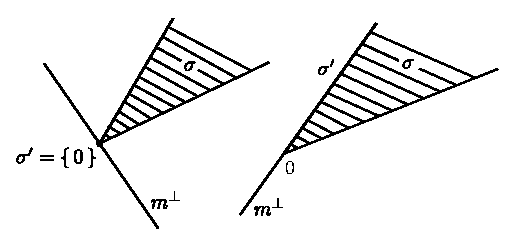
\includegraphics{vol58-fig/fig58-2.eps} 
\end{figure}

\end{defi*}


\begin{defi*}
{\em A rational\pageoriginale partial polyhedral decomposition}
(r.p.p. decomposition, 
for short) is a pair $(N, \Delta)$ consisting of a free
$\mathbb{Z}$module $N$ of finite rank and a collection $\Delta$ of
cones in $N_{\mathbb{R}}$ such that $(i)$ if $\Delta \ni \sigma,
\sigma > \tau $, then $\tau \in \Delta$ and $(ii)$ if $\sigma$ and
$\tau$ belong to $\Delta$, then the intersection $\sigma \cap \tau $
is a face of $\sigma$ as well as of $\tau . (N, \Delta)$ is called a
\textit{finite rational partial polyhedral
  decomposition}(f. r. p. p. decomposition for short ) if $\Delta$ is
finite.  
\end{defi*}

	The relative interiors of $\sigma \in \Delta$ are disjoint and
        fill a part of $N_{\mathbb{R}}$. When rank $N = 2, \Delta$
        looks like this: 

\begin{figure}[H]
\centering 
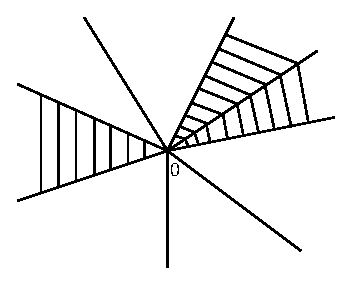
\includegraphics{vol58-fig/fig58-3.eps} 
\end{figure}

\begin{defi*}
A map $h : (N , \Delta ) \to (N' , \Delta' )$ between
r.p.p. decompositions is a $\mathbb{Z}$- homomorphism $h : N \to N'$
with 
\textit{ finite cokernel } such that for each $\sigma \in \Delta$,
there exists $\sigma' \in \Delta'$ with the scalar extension $ h :
N_{\mathbb{R}}\rightarrow N_{\mathbb{R'}} $ satisfying $ h(\sigma)
\subset \sigma' $. Thus we have the category of r.p.p. decompositions. 
\end{defi*}

\begin{defi*}
A cone $\sigma$ in $N_{\mathbb{R}}$ is called \textit{ simplicial } if
its fundamental generators $n_1, \ldots, n_s$ are ${\mathbb{R}}$-
linearly independent. $\sigma$ is called \textit{ non- singular} if
its fundamental generators form a part of a ${\mathbb{Z}}$-basis if
$N$.  
\end{defi*}

Given\pageoriginale a strongly convex rational polyhedral cone
$\sigma$ in $N_{\mathbb{R}}$, we denote by $\check{\sigma}$ its dual in 
$M_{\mathbb{R}}$ 
$$
\check{\sigma} = \Big\{\ x \in M_{\mathbb{R}} ; \langle x, y\rangle
\geq \text{ for all} y \in \sigma\Big\},  
$$ 
where $M = N^*$ is the dual of $N$. $\check{\sigma}$ can be written as
the set of $\mathbb{R}_\circ$-linear combinations of a finite number
of elements of $M$ and is a convex rational polyhedral cone, although
it no longer satisfies the strong convexity $\check{\sigma} + (
-\check{\sigma}) = \Big\{\ 0 \Big\}$. Instead, it satisfies
$\check{\sigma} + ( -\check{\sigma}) M_{\mathbb{R}}$. For the general
theory convex polyhedral cones, we refer the reader for instance to
Gr\"{u}nbaum \cite{keyG3} and Rockafellar \cite{keyR3}.  

For a subset $\tau$ of $\sigma$, we denote 
$$
\tau^{\perp} = \Big\{ \ x \in M_{\mathbb{R}} ; \langle x , y \rangle =
0 \text{ for all } y \in \tau \Big\}.  
$$

\noindent
Then $y \in \sigma$ is in relative interior of $\sigma$ if and only if
$\check{\sigma} \cap y^{\perp} = \sigma^\perp $, i.e for all $x \in
\check{\sigma}$ not in $\sigma^\perp$, we have $ \langle x, y \rangle
> 0$ 

The following propositions will be useful later. 

\setcounter{prop}{0}
\begin{prop}\label{chap1:prop3.1} %Prop 3.1
Let $\sigma$ be a cone in $N_{\mathbb{R}}$ and $\check{\sigma}$ be its
dual in $M_{\mathbb{R}}$. Then the map  
$$
\tau \longmapsto \check{\sigma} \cap \tau^\perp
$$
is na order reversing bijection 
$$
\Big\{ \text{ faces of } \sigma \Big\} \xrightarrow{\sim}\Big\{ \text{
  faces of } \check{\sigma} \Big\}. 
$$
\end{prop}

\begin{proof}
By definition, a face of $\check{\sigma}$ is of the form
$\check{\sigma} \cap y^\perp$ for $y \in \sigma$. $y$ belongs to the
relative interior of a face $\tau$ of $\sigma$ if and only if
$\check{\tau} \cap y^\perp= \tau^\perp $ , i.e. $\check{\sigma} \cap
\tau^\perp$.  
\end{proof}

\begin{prop}\label{chap1:prop3.2} %Prop 3.2
Let $\sigma$ be a come in $N_{\mathbb{R}}$ and $\tau$ a face of $\sigma$. 
Then\pageoriginale there exists $x \in \check{\sigma} \cap \tau^\perp$
such that  
$$
\check{\tau}= \check{\sigma} + \tau^\perp = \check{\tau} +
\mathbb{R}_\circ (-x).  
$$
\end{prop}

\begin{proof}
Since $\tau$ is a face of $\sigma$, there exists $x \in
\check{\sigma}$ such that $\tau =\sigma \cap x^\perp$. We have
inclusions $\check{\tau} \supset \check{\sigma} + \tau^\perp \supset
\check{\sigma} + \mathbb{R}_\circ (-x)$ of convex polyhedral cones in
$M_{\mathbb{R}}$. The dual $\tau$ of the first and the dual $\sigma
\cap \mathbb{R}_\circ (-x)^{\vee} = \sigma \cap x^\perp$ of the third
coincide, and we are done.  
\end{proof}

\begin{prop}\label{chap1:prop3.3} %Prop 3.3
The correspondence 
$$
\sigma \longmapsto \check{\sigma} \cap M
$$
establishes a bijection between the set of strongly convex rational
polyhedral cones in $N_{\mathbb{R}}$ and the set of subsemigroups $S$
of $M$ which satisfy the following properties:  
\begin{enumerate}[(1)]
\item $S \in 0$ and is finitely generated as a semigroup. 

\item $S$ generates $M$ as a group.  

\item $S$ is saturated, i.e. $S$ contains $ m \in M$ if there
  exists a positive integer a such that $am \in S$.  
\end{enumerate}
\end{prop}

\begin{proof}
$\check{\sigma} \cap M$ obviously contains 0 and is a saturated
  subsemigroup. Since $\sigma \cap (- \sigma) = \{ 0\}$ by definition,
  we have $\check{\sigma} + \check{(-\sigma)} = M_{\mathbb{R}}$, hence
  $(ii)$. The finite generation of $\check{\sigma} \cap M$ as a
  semigroup is what is known as Gordan's lemma and can be proved as
  follows : We may assume that $\check{\sigma}$ is of the form
  $\mathbb{R}_\circ m_1 +\cdots + \mathbb{R}_\circ m_s$ for
  $\mathbb{R}$-linearly independent elements $m_1 , \ldots , m_S \in
  M$, since general $\check{\sigma}$ is a finite union of convex cones
  of this form by Carathoeodry's theorem (see for instance
  Gr\"{u}nbaum  \cite{keyG3}). Let $M' = M \cap (Qm_1+\cdots+ Qm_S)$. Then
  $\check{\sigma}\cap M = \check{\sigma} \cap M'$\pageoriginale and
  $M''=\mathbb{Z} m_1+\cdots+\mathbb{Z} m_s$, is a submodule of finite
  index in $M'$. Since $\check{\sigma} \cap M' = \mathbb{Z}_\circ m_1
  + \cdots + \mathbb{Z}_\circ m_s $, we are done. Conversely, let 
  $S$ satisfy (i), (ii) and (iii). By (i), there exist elements
  $m_1 , \ldots, m_s \in M$ such that $\mathbb{Z}_\circ m_1 +\cdots +
  \mathbb{Z}_\circ m_S$. Then $\check{\sigma} = \mathbb{R}_\circ m_1
  +\cdots + \mathbb{R}_\circ m_s$ is a convex rational polyhedral cone
  in $M_{\mathscr{R}}$ satisfying $\check{\sigma} + (-\check{\sigma})
  = M_{\mathbb{R}}$. Hence $\check{\sigma} = \check{\check{\sigma}} $ is a
  strongly convex rational polyhedral cone. It remains to show that $S
  = \check{\sigma} \cap M$. Again by Caratheodory's theorem, and
  element in $\check{\sigma} \cap M$ is a $Q_\circ$ linear
  combinations of $m_1 ,\ldots , m_s$. Thus a positive integral
  multiple of it is contained is $S$. Hence we are done by (iii).  
\end{proof}

\section{First main theorems}\label{chap1:sec4}

	For later convenience, we state the first main theorems
        relating torus embeddings and r.p.p. decompositions in this
        section, and leave their proofs of \S. \ref{chap1:sec5}.  

	The following theorem is slightly more general than those in
        Demazure \cite[\S. \ref{chap1:sec4}]{keyD2}, Mumford et
        al.\cite[I.2, Thm.6]{keyTE} 
        and Miyake-Oda \cite{keyMO}.  

\begin{theorem}\label{chap1:thm4.1} %theorem 4.1
Given $k$, there exists an \textit{equivalence} of categories
\begin{gather*}
\big\{\text{ r.p.p.decompositions} \big\} \longrightarrow 
\left.
\begin{cases}
\text{normal and separated torus} \\
\text{embeddings over $k$} \\
\text{locally of finite type} 
\end{cases} 
\right\}\\
(N, \Delta) \longmapsto T_N\subset T_N \emb (\Delta)
\end{gather*}
where\pageoriginale $T_N = N \otimes_{\mathbb{Z}} k^* = \Hom_{gr}
(N^*, k^*) $ and $T_N emb (\Delta)$ is obtained as the canonical
patching of its affince open subsets   
$$
\Hom_{\text{unit.semigr}} (\check{\sigma} \cap N^*, k).  
$$
Here $k$ is considered as a unitary semigroup under the \textit{
  multiplication} and $T_N$ acts on it by $(tx)(m) = t(m)x(m)$ for $t
\in T_N$, $m \in N^*$ and $x \in
\Hom_{\text{unit.semigr}}(\check{\sigma}\cap N^*, k)$.

 $T_N \emb(\Delta)$ is of finite type over $k$ if and only if $\Delta$
is finite.   
\end{theorem}

\begin{remark*}
This down-to-earth description of the functor as well as the
simplified proof in \S. \ref{chap1:sec5} was pointed out by Ramanan.  
\end{remark*}

\begin{theorem}\label{chap1:thm4.2} %Theorem 4.2
Let $(N, \Delta)$ be an r.p.p decomposition. 
\begin{enumerate}[(i)]
\item The map 
$$
\sigma \longmapsto \orb (\sigma) = \Hom_{gr} (\sigma^\perp \cap N^*, k^*)  
$$
is a bijection 
$$
\orb : \Delta \xrightarrow{ \sim} \Big\{\ T_N- \text{orbits in } T_N
\emb (\Delta)\Big\},  
$$
such that $\orb (\{0\})= T_N$ and $\dim \sigma + \dim \orb (\sigma) =
\dim T_N$. Moreover, $\tau < \sigma $ if and only if the closure of
$\orb(\tau)$ contains orb$(\sigma)$.  

\item The map
$$
\sigma \longmapsto U (\sigma) = \coprod_{\tau < \sigma} \orb (\tau) = 
\Hom_{\text{unit.semigr}} (\check{\sigma} \cap N^*, k ) 
$$
establishes an order and intersection preserving bijection $\Delta
\xrightarrow {\sim}$\pageoriginale \{$T_N$-stable affine open sets in
$T_N \emb (\Delta)$\}. In particular, $T_n \emb (\Delta)$ is
\textit{affine} if and only if $\Delta$ consists of the faces of a
fixed cone in $N_\mathbb{R}$.  

\item For $\sigma \in \Delta$, let $\bar{N}$ be the quotient of $N$ by
  the subgroup generated by $\sigma \cap N$. Then $T_{\bar{N}} =
  \Hom_{gr} (\sigma^\perp \cap N^\ast, k^\ast)$. The closure
  $\overline{\orb(\sigma)}$ of $\orb(\sigma)$  in $T_N \emb(\Delta)$
  is normal and 
$$
\overline{\orb (\sigma)} = \coprod\limits_{\sigma < \tau\in
    \Delta} \orb (\tau).  
$$
\end{enumerate}

It coincides with $T_{\overline{N}}\emb (\Delta)$, where $\bar{\Delta}$ is the
r.p.p.decomposition of $\overline{N}_{\mathbb{R}}$ consisting of the
images $\overline{\tau}$ of $\sigma < \tau \in \Delta$ under
$N_{\mathbb{R}} \to \overline{N}_{\mathbb{R}}$.  
\end{theorem}

\begin{theorem}\label{chap1:thm4.3} % Theorem 4.3 
Let $(N,\Delta)$ be an r.p.p.decomposition. Then the corresponding
$T_N \emb(\Delta)$ is \textit{non-singular} if and only if each
$\sigma \in \Delta$ is non-singular, i.e. its fundamental generators
of each form a part of a $\mathbb{Z}$-basis of $N$. In this case, the
closure of each  $T_N$-orbit orb $(\sigma)$ is again non-singular.  
\end{theorem}

\begin{remark*}
When $T_N \emb (\Delta)$ is non-singular, the collection of the sets
fundamental generators of $\sigma$ with running through $\Delta$ is a
``fan'' of Demazure \cite[\S. \ref{chap1:sec4}, $n^\circ$.2]{keyD2}. 
\end{remark*}

\begin{theorem}\label{chap1:thm4.4} %Theorem 4.4 
Let $h: (N,\Delta)\longrightarrow (N', \Delta')$ be a map of
r.p.p. decompositions, and let $f:T_N \emb (\Delta) \to T_{N'} \emb
(\Delta')$ be the corresponding equivariant dominant morphism. Then $f$ is
\textit{proper} if and only if for each $\sigma' \in \Delta'$ the set
$\Big\{ \sigma \in \Delta ; h (\sigma) \subset \sigma' \Big\}$ is
finite and $h^{-1}(\sigma')$ is the of its members.  
\end{theorem}

\setcounter{coro}{4}
\begin{coro}\label{chap1:coro4.5} % Coro 4.5
Let\pageoriginale $(N, \Delta)$ be an r.p.p.decomposition. Then $T_N
\emb (\Delta)$ is \textit{complete} (i.e. proper over Spec $k$), if
and only if $\Delta$ is finite and   
$$
N_{\mathbb{R}} = \bigcup_{\sigma \in \Delta} \sigma.
$$
\end{coro}

\section{The proof of theorems in $\S.4$}\label{chap1:sec5}

	In this section, we prove theorems stated in \S. \ref{chap1:sec4} in a way
        slightly different from Mumford et al.\cite{keyTE}. We informally deal
        with $k$-valued points only, although, to be rigorous, we should
        deal with points with values in arbitrary $k$-algebras.  
	
	Here is the \textit{key observations} relating cones and
        normal affine torus embeddings. We were inspired by Hochster
        \cite{keyH5}.  
	
\subsection{}\label{chap1:subsec5.1}
 Let $N$ and $M$ be mutually dual free $\mathbb{Z}$-modules of finite
rank with the pairing $< , >$. Let $T = T_N = N \otimes_{\mathbb{Z}}
k^*$. Then the correspondence  
$$
\sigma \longmapsto U(\sigma) = \Hom_{unit.semigr} (\check{\sigma} 
\cap M, k^*) 
$$
is a bijection from the set of (strongly convex rational polyhedral)
cones $\sigma \subset N_{\mathbb{R}}$ to the set of \textit{normal
  affine} $T_N$-embeddings (of finite type) over $k$.  

\begin{proof}
By Proposition \ref{chap1:prop3.3}, $\check{\sigma}\cap M$ is a finitely generated
saturated subsemigroup of $M$ which generates $M$ as a group. Thus its
semi group algebra $A = A (\sigma) = \bigoplus\limits_{m \in
  \check{\sigma} \cap M} ke (m)$ is a subalgebra of finite
type\pageoriginale of the  
coordinate ring $k[T] = \bigoplus\limits_{m \in M} ke (m)$ of $T$. It is
$T$-stable under algebraic representation of $T$ on $k[T]$ defined by
$f(t) \longmapsto f(t' t)$ for $f(t) \in k[T]$ and $t'\in
T$. Since $\check{\sigma} \cap M$ generates $M$ as a group, the
quotient field of $A$ coincides with the quotient field $k(T)$ of
$k[T]$. Since $\check{\sigma} \cap M$ is saturated, $A$ is integrally
closed in $k(T)$. Indeed, the integral closure $A'$ is of finite type
over $k$, hence the representation of $T$ on $A'$ as above is also
algebraic. Thus by the complete reducibility theorem, $A'$ has a
$k$-basis consisting of elements of the form $e(m')$ with $m' \in
M$. $e(m')$ satisfies an equation  
$$
e(m')^c + a_1 e(m')^{c-1} +\cdots + a_c =0  
$$
with $a_i$ in $A$, which we may assume to be a $k$-multiple of an
element $e(m_i), m_i \in \check{\sigma} \cap M$. Obviously there
exists a non-vanishing $a_i$. Then we have $cm'= m_i + (c-i)m' $,
i.e. $im' = m_i \in \check{\sigma} \cap M $, hence $m' \in
\check{\sigma}\cap M$. A ($k$-valued) point of $U(\sigma) =$ Spec $A$
is a k=algebraic homomorphism $ u : A \to K$, which is determined
uniquely by $u(e(m))\in k$ for $m \in M$, such that $u(e(0))=1$ and
$u(e(m+m'))= u(e(m))u(e(m'))$, i.e., $u \circ e: M \to K $ is a
homomorphism of unitary semigroups. $T$ obviously acts on $U(\sigma)$ as
in the statement of Theorem \ref{chap1:thm4.1}. Let $m_1, \ldots m_s$
be generators 
of $\check{\sigma} \cap M$ as a semigroup. Then $M$ is generates by
$m_1 , \ldots , m_s$ and $-(m_1 + \cdots + m_s)$. Thus $k[T]$ is the
localization of $A$ by $e(m_1 + \cdot + m_s)$. Hence $U(\sigma)$
contains $T$ as an open set.  
\end{proof}

 Conversely, let $T  \subset$ Spec $A$ be a normal affine $T$-embedding
 of finite\pageoriginale type. Hence $A$ is a $k$-subalgebra of finite
 type of 
 $k[T]$, is normal with the quotient field $k(T)$ and is $T$-stable
 under the algebraic representations of $T$ on $k[T]$ and is $T$-stable
 under the algebraic representations of $T$. Thus by the complete
 reducibility, it has a $k$-basis consisting of $T$-semi invariants,
 i.e. $A = \bigoplus\limits_{m\in S} ke(m)$ for a finitely generated
 subsemigroup $S \ni 0$ of $M$. $S$ generates $M$ as a group. Indeed,
 for $m' \in M$, the denominator ideal of $e(m')$ is a non-zero
 $T$-stable ideal of $A$, hence contains some $e(m) $with $m \in S$, and
 $e(m) e(m') \in A$. $S$ is obviously saturated, since $A$ is
 integrally closed in $k(T)$. Hence by proposition
 \ref{chap1:prop3.3}, there exists 
 a unique cone $\sigma \subset N_\mathbb{R}$ such that $ S =
 \check{\sigma}\cap M$.  

\begin{remark*}
Non-normal affince $T_N$-embedding can also be written as  
$$
Spec (\bigoplus\limits_{m \in S} ke (m)) 
$$
for a subsemigroup $S \ni 0 $ which generates $M$ as a group. The
simplest non-trivial example is the curve Spec $(k [t^2 , t^3])$ with
an ordinary cusp. In this case, $M = \mathbb{Z}$, and $S$ is generates
by 2 and 3. In general, it is difficult to describe such
non-saturated $S$. For the special case of dimension one, we refer the
reader to Delorme \cite{keyD1}, Herzog \cite{keyH2} and Herzog-Kunz
\cite{keyHK}.   
\end{remark*}

\subsection{}\label{chap1:subsec5.2}%%% 5.2
 Let $h : N \to N'$ be a homomorphism with finite
cokernel and let $f:T_N \to T_N'$ be the corresponding surjective
homomorphism of algebraic tori. Let $T_N \subset U(\sigma)$ and
$T_{N'} \subset U (\sigma')$ be the
normal affine torus embeddings corresponding to cones $\sigma \subset
N_\mathbb{R}$ and $\sigma' \subset N'_\mathbb{R}$ as 
in\pageoriginale (\ref{chap1:subsec5.1}). Then $f$ can be extended to a unique
equivariant dominant 
morphism $\bar{f}: U (\sigma) \to U(\sigma')$, if and only if of the
scalar extension $h : N_\mathbb{R}\to N'_\mathbb{R}$ satisfies
$h(\sigma) \subset \sigma'$.  

\begin{proof}
Let $M$ and $M'$ be the duals of $N$ and $N'$, respectively. Then $h$
induces an injection $h^* : M' \to M$, which gives rise to $f : T_N =
\Hom_{gr}(M, k^*) \to T_{N'} = \Hom_{gr} (M', k^*)$. Obviously,
$h(\sigma \leq) \subset \sigma'$ if and only if 
$h^*(\check{\sigma}' \cap M') \subset \check{\sigma}\cap M$, and in
this case it induces a morphism $\bar{f}: U(\sigma)=
\Hom_{unit.semigr}(\check{\sigma}\cap M, k)\longrightarrow U(\sigma')
= \Hom_{unit.semigr} ( \check{\sigma}'\cap M', k)$.  
\end{proof}

\subsection{}\label{chap1:subsec5.3}%% 5.3
 Let $\sigma$ be a cone in $N_{\mathbb{R}}$ and let $M$ be the
dual of $N$. Then the corresponding normal affine
$T_N$-embedding $U(\sigma)= \Hom_{unit. semigr} ( \check{\sigma}
\cap M, k)$ is the disjoint union of $T_N$-orbits  
$$
\orb (\tau) = \Hom_{gr}(\tau^\perp \cap M, k^*) 
$$
with $\tau$ running through the faces of $\sigma$. The closure of orb 
$\tau$ in $U(\sigma)$ is  
$$
\overline{\orb (\tau)} = \Hom_{unit. semigr}(\check{\sigma} \cap
\tau^\perp \cap M, k) 
$$
and it is the disjoint union of $\orb \tau'$ with $\tau'$ running
through the faces of $\sigma$ with $\tau < \tau' $. 

\begin{proof}
The following argument, which considerably simplifies our original
proof, is due to Ramanan. For simplicity, we denote $ S=
\check{\sigma} \cap M$. Let $g : S \to k $ be a unitary semigroup
homomorphism, i.e. $g(0)=1$ and $g(m+m')$ for $m, m' \in S$. Then $S$
is the disjoint union of $I = g^{-1}(0)$ and $S' = g^{-1}(k^*)$. $S'$
is a subsemigroup\pageoriginale  containing 0 of $S$ and $S + I
\subset I$. We first show that a decomposition $S = S' \coprod I$ is
obtained exactly by 
taking a face $F$ of $\check{\sigma}$ and letting $S' = F \cap
M$. Indeed, if $F$ is a face of $\check{\sigma}$, there exists $y \in
\sigma$ such that $F = \check{\sigma}\subset y^\perp$. Certainly, $F
\cap M$ is a subsemigroup containing 0 of $S$, and for $z$ and $w$ in
$S$ with $w$ not in $F \cap M$, $z+w$ is not in $F\cap M$.   
\end{proof}

	Conversely, let $S'$ be a subsemigroup containing 0 of $S$
        such that its complement $I$ satisfies $S + I \subset
        I$. Hence $m \in S$ is in $S'$ of $(S+m) \cap S' \neq
        \phi$. Replacing $\check{\sigma}$ by its smallest face
        containing $S'$, we may assume that there exists $m' \in S'$
        in the relative interior of $\check{\sigma}$. We claim
        $(S+m)\cap \mathbb{Z}_\circ m' \neq \phi$ for $m \in S$, hence $m
        \in S'$ by assumption and $\mathbb{Z}_\circ m' \subset
        S'$. Indeed, since $m'$ is in the
        relative interior of $\check{\sigma}$, we see that $ \langle
        m', n_i \rangle > 0$ for the fundamental generators $n_1,
        \ldots , n_s$ of $\sigma$. Thus $S+m= \{ m'' \in M ; < m'' n_i>
        \geq < m, n_i> \text{ for } 1 \leq i \leq s \}$. Choose a
        positive integer a such that $a<m'$, $n_i> \geq <m$,
        $n_i>$for $1\leq i \leq s$. Then $am'$ is in $S+m$.  
 	 
	By proposition \ref{chap1:prop3.1}, we know that $F= \check{\sigma}\cap
        \tau^\perp$ for a unique face $\tau$ of $\sigma$. Thus we see
        that $\Hom_{\text{unit.semigr}} (\check{\sigma} \cap M, k)=
        \coprod\limits_{\tau < \sigma}
        \Hom_{\text{unit.semigr}}(\check{\sigma}\cap \tau^\perp \cap
        M)$ 
        generates $\tau^\perp \cap M$ as a group, hence
        $\Hom_{\text{unit. semigr}}(\check{\sigma}\cap \tau^{\perp}\cap M,
        k^*)= \Hom_{gr}(\tau^\perp \cap M, k^*)= T_N\cdot \varepsilon
        (\tau)$, where $\varepsilon (\tau)$ is the trivial group homomorphism 
        $\tau^\perp \cap M \to k^*$ sending\pageoriginale  every element
        to 1. Let $A= \bigoplus_{m\in\check{\sigma}\cap M}
        ke (m)$ and   
$$ 
\mathbb{P} (\tau) = \bigoplus\limits_{\substack{m \in \check{ \sigma} 
    \cap M     \\  m \notin \check{\sigma} \cap \tau^\perp \cap M} }  ke(m) .  
$$
Then $\mathbb{P} (\tau)$ is a prime ideal of $A$ with the subring
$\underset{ m \in \check{\sigma} \cap \tau^\perp M}{\oplus} ke (m)$
isomorphic to $A/ \mathbb{P}(\tau)$. $\Hom_{\text{unit. simigr}}
(\check{\sigma} \cap \tau^\perp \cap M, k)$ is obviously the disjoint
union of orb $(\tau')$ 
with $\tau'$ running through the faces of $\sigma$ with $\tau < \tau'$
and is precisely (the set of $k$-valued points of) the closed set
Spec $(A/\mathbb{P} (\tau))$. 

\begin{remark*}
Let $A$ and $\mathbb{P} (\tau)$  be as above. Then the correspondence 
$$
\tau \longmapsto \mathbb{P} (\tau) 
$$
establishes an order preserving bijection 
$$ 
\left\{\text{ faces of } \sigma \right\} \xrightarrow{\sim} \left\{
T_N - \text{ stable prime ideals of A} \right\}.    
$$

 $\mathbb{P}(\sigma)$ is the largest $T_N$-stable proper ideal of
$A$. Let $n_1 , \ldots, n_s $ be the fundamental generators of
$\sigma$, hence $\mathbb{R}_o n_1 ,\ldots, \mathbb{R}_o n_s$ are the
one-dimensional faces of $\sigma$. Then $\mathbb{P}(\mathbb{R}_o n_1)
,\ldots, \mathbb{P}(\mathbb{R}_o n_s)$ are the $T_N$-stable height one
prime ideals of $A$. The localization $A_{\mathbb{P}(\mathbb{R}_o n_i)}$
is a discrete valuation ring, hence we have a surjective homomorphism
ord$_i: k(T)^*  \to \mathbb{Z}$, valuation ring onto
$\mathbb{Z}_\circ$. Composed with $e: M \to k(T)^*$, it gives rise to a
surjective homomorphism $\ord_i \circ e : M \to \mathbb{Z}$, which is
exactly the primitive element $n_i \in N$. 
\end{remark*}

\subsection{}\label{chap1:subsec5.4}%%(5.4)
 Let\pageoriginale $\sigma \subset N_{\mathbb{R}}$ be a cone and
let $U(\sigma) = \Hom_{\text{unit.semigr}}(\check{\sigma} \cap M, k)$ be
the corresponding normal affine $T_N$-embedding. Then the map  
$$
\tau \longmapsto U(\tau) =   Hom_{\text{unit.semigr}} (\check{\tau}
\cap M, k) 
$$
 is a bijection
$$
\{ \text{faces of } \sigma \} \xrightarrow{\sim} \{ T_N- \text{
   stable affine open subsets of } U(\sigma) \}.
$$ 
Moreover, we have $U(\tau) = \prod\limits_{\tau ' < \tau } \orb
(\tau')$.  

\begin{proof}
Let $A = \bigoplus\limits_{ m \in \check{\sigma}\cap M} ke (m)$ so
that $U(\sigma) = \Spec(A)$. If $\tau$ is a face of $\sigma$, there
exists, by proposition \ref{chap1:prop3.2}, an element $m_0 \in
\check{\sigma} \cap 
\tau^{\perp}\cap M$ such that $\check{\tau} \cap M = 
(\check{\sigma} \cap M) + \mathbb{Z}_\circ  (-m_0)$. Hence
$\bigoplus\limits_{m \in 
 \check{\tau} \cap M} ke(m) = A[ e(m_0)^1]$, whose spectrum
$U(\tau)$ is obviously a $T_N$-stable affine open set. 
\end{proof}

Conversely, let $\spec B$ be a $T_N$-stable affine open set of
$U(\sigma)$. Then by (\ref{chap1:subsec5.1}), There exists a cone $\tau \subset
\sigma$ in $N_{\mathbb{R}}$ such that $\{ e(m) ; m \in \check{\tau}
\cap M \}$ form a $k$-basis of $B$. It remains to show that $\tau$ is
a face of $\sigma$. The following argument is again due to
Ramanan. Replacing $\sigma$ by its smallest face containing $\tau$, we
may assume that there exists $ n \in \tau \cap N$ in the relative
interior of $\sigma$. Then $\check{\tau} \cap n^{\perp}$ is face of
$\check{\sigma}$ and its intersection with $\check{\sigma}$ is exactly
$\check{\sigma} \cap n^{\perp} = \sigma^{\perp}$. Thus the ideal
$\mathbb{P}(\sigma)B$ generated by the prime ideal
$\mathbb{P}(\sigma)$ of $A$  is a proper ideal of $B$. Thus
orb$(\sigma) =  \spec (A/\mathbb{P}(\sigma))$ is contained in the
$T_N$-stable affine open set $\spec B$. Since the closure of any
$T_N$-orbit in $U(\sigma)$ contains orb$(\sigma)$ by (\ref{chap1:subsec5.3}), any
$T_N$-orbit in $U(\sigma)$ is contained in $\spec B$ and we are
done. $U(\tau)$ is the disjoint union of $\orb(\tau')$, $\tau' < \tau$,
by (\ref{chap1:subsec5.3}). 

Combining\pageoriginale (\ref{chap1:subsec5.3}) and
(\ref{chap1:subsec5.4}), we have the following:    

\subsection{}\label{chap1:subsec5.5}%% 5.5
Let $\sigma \subset N_{\mathbb{R}}$ be a cone and let
$U(\sigma) = \Hom_{\text{unit.semigr}} (\check{\sigma} \cap M, k)$ be the
corresponding normal affine $T_N$-embedding. Then 
$$
\tau \longmapsto \orb(\tau) =  \Hom_{gr} (\tau^{\perp} \cap
M, k^*) 
$$
 is a bijection
 $$
  \orb: \{ \text{faces of } \sigma \} \xrightarrow{\sim} \{ T_N-
  \text{orbits in } U(\sigma) \} .
 $$
  Moreover,
  $$
  \tau \longmapsto U(\tau) = \Hom_{\text{unit.semigr}} (\check{\tau} 
  \cap M, k) 
  $$
   is a bijection  
 $$
\{ \text{faces of } \sigma \} \xrightarrow{\sim} \{
T_N-\text{stable affine open subsets of } U(\sigma) \}.  
$$
   
\noindent
For each $\tau < \sigma$, they satisfy the following properties :  
\begin{enumerate}[(i)]
\item $\dim \tau + \dim \orb (\tau) = \dim T_N$, $\orb (\{ 0 \}) =
  T_N$ and $\orb(\sigma)$ is the unique closed orbit of $U(\sigma)$. 

\item $U(\tau) = \underset{\tau' < \tau }{\coprod} \orb (\tau)$

\item The closure of $\orb (\tau)$ in $U(\sigma)$ is
$$
\overline{\orb (\tau)} = \underset{\tau < \tau' < \sigma}{\coprod} \orb 
  (\tau')= \Hom_{\text{unit.semigr}} (\check{\sigma} \cap \tau^{\perp} \cap M,
k). 
$$
It is the normal affine embedding of $\orb (\tau)=\Hom_{gr} (t^{\perp}
\cap M, k^*)$ corresponding to the image of $\sigma$ under the map
from $N_{\mathbb{R}}$ to its quotient by the subspace $\sigma + (-
\sigma)$ generated by $\sigma$. 

\item The morphism $\rho_{\tau} : U(\sigma) \to \overline{\orb
  (\tau)}$ induced by the inclusion $\check{\sigma}\cap \tau^{\perp} \cap
  M \hookrightarrow \check{\sigma} \cap M$ is a retraction
  such that $U(\tau)= \rho_{\tau}^{-1}(\orb(\tau))$. 
\end{enumerate}

\begin{remark*}
The map orb can also be described as in Mumford et al. \cite{keyTE} as
follows : For $t \in k^*$ and $n \in N$, consider the element
$\tau^{\langle ?,  n \rangle}$ of $T_N =
\Hom_{gs}(M,k^*)$.\pageoriginale Let $U(\tau)= 
\Hom_{\text{unit. semigr}} (\check{\sigma}  \cap M, k)$ be the normal affine
$T_N$-embedding. The limit of  $t^{ \langle ?, n \rangle}$ as $t$ tends to zero
exists in $U(\sigma)$ if and only if $ \langle m,n \rangle \geq 0$ for all $m \in
\check{\sigma}  \cap M $, i.e. $n \in \sigma \cap N$. In that case,
the limit is the semigroup homomorphism form $\check{\sigma}  \cap M$
to $k$ sending those $m$ with $\langle m,n \rangle =0$ to $1 \in k$
and those with 
$\langle  m, n \rangle > 0$ to $0 \in k$, i.e. the identity element $\varepsilon
(\tau)$ of $\orb(\tau)= \Hom_{gr}(\tau^{\perp} \cap M, k^*)$, where
$\tau$ is the face of $\sigma$ containing $n$ in its relative
interior, by Proposition \ref{chap1:prop3.1}. 
\end{remark*}

\subsection{}\label{chap1:subsec5.6}%% (5.6)
  Let $\sigma \subset N_{\mathbb{R}}$ correspond to the normal
affine $T_N$-embedding\break $U(\sigma)= \spec A$. Let  $\mathbb{P}(\sigma)$
be the largest $T_N$-stable proper ideal of $A$ as in the remark after
(\ref{chap1:subsec5.3}). Then the following are equivalent: 
\begin{enumerate}[(i)]
\item $U(\sigma)$ is non-singular.

\item The local ring $A_{\mathbb{P}(\sigma)}$ is regular.

\item $\sigma$ is non-singular, i.e. the fundamental generators of
  $\sigma$ form a part of a $\mathbb{Z}$-basis of $N$.
\end{enumerate}

\begin{proof}
$(i)$ obviously implies $(ii)$. Let us assume $(ii)$ and show
  $(iii)$. Obviously, there exist $m_1,\ldots, m_s$, $s=$ height
  $(\mathbb{P}(\sigma))$, such that $\{ e(m_1) ,\ldots,\break e(m_s) \}$ is
  a minimal set of generators of the maximal ideal of the local
  ring. It is easy to see that $e(m)$, $m \in M$ is contained in the
  local ring if and only if $m \in \check{\sigma} \cap  M$. But such
  $m$ can be written uniquely as $m = m_0 + a_1 m_1 + \cdots + a_s
  m_s$ with $a_i \in \mathbb{Z}o$ and\pageoriginale $m_0 \in
  \sigma^{\perp} \cap 
  M$. Hence a $\mathbb{Z}$-basis of $\sigma^{\perp} \cap M$ together
  with $m_1, \ldots, m_s$ form a $\mathbb{Z}$-basis of $M$. Among the
  dual basis of $N$, we can choose $n_1 , \ldots , n_s \in \sigma$
  such that $\langle m_i ,n_j \rangle = \delta_{ij}$. Then $\sigma = \mathbb{R}_o
  n_1 + \cdots + \mathbb{R}_o n_1$. It remains to show that $(iii)$
  implies $(i)$. Let the fundamental generators $n_1 ,\ldots, n_s$ of
  $\sigma$ be extended to a $\mathbb{Z}$-basis $n_1 , \ldots , n_r$ of
  $N$. Let $m_1 , \ldots , m_r$ be the dual basis of $M$. Then
  $\check{\sigma} \cap M = (\mathbb{Z}_o m_1 + \cdots + \mathbb{Z}_o
  m_s) + (\mathbb{Z} m_{s+1} + \cdots + \mathbb{Z} m_r)$, hence $A= k[
    u_1, \ldots , u_r,u^{-1}_1,\ldots u^{-1}_s]$ with $u_i = e(m_i)$,
and $\spec A$ is non-singular. 
\end{proof}

\subsection{}\label{chap1:subsec5.7}%% (5.7)
\medskip
\noindent{\textbf{Proof of Theorem 4.1}}
Let $(N , \Delta)$ be an r.p.p.decomposition.
Let $M = N^*$ be the dual of $N$. For $\sigma \in \Delta$, let
$U(\sigma) = \Hom_{\text{unit.semigr}} (\check{\sigma} \cap M,k)$ be the
corresponding normal affine open $T_N$embedding of finite type. For
$\sigma , \tau \in \Delta , \sigma \cap \tau $ is a face of $\sigma$
and $\tau$. Thus by (\ref{chap1:subsec5.4}), $U(\sigma \cap \tau)$ is
canonically a 
$T_N$-stable affine open set of $U(\sigma)$ and $U(\tau)$. Thus we can
paste $U(\sigma)$'s together along $U(\sigma \cap \tau )$ to obtain an
irreducible normal scheme $T_N \emb (\Delta)$ locally of finite
type. Obviously, $T_N$ acts algebraically on it with the dense orbit
$U(\{ 0 \})= T_N$. It is separated, since $U(\sigma) \cap U(\tau) =
U(\sigma \cap \tau)$ is an affine open set and the coordinate ring of
$U(\sigma \cap \tau)   $ is generated by those of $U(\sigma)$ and
$U(\tau)$. Indeed, they $k$-bases consisting of elements of the form
$e(m)$ and $(\check{\sigma} \cap M) + (\check{\tau} \cap M)= (\sigma
\cap \tau)^v \cap M $. 


A map $h : ( N, \Delta) \to (N' , \Delta')$ of $r.p.p$. decompositions
obviously gives rise to an equivariant dormant morphism $f : T_N$
emb$(\Delta) \to T_{N'}\break emb (\Delta')$. On the other hand, suppose $f$ is
given. It induces\pageoriginale $h: N \to N'$. Then for $ \sigma \in
\Delta$, the 
unique closed $T_N$-orbit orb $(\sigma)$ of $U (\sigma)$ is mapped by
$f$ to a $T_N'$-orbit $f(\orb(\sigma))=  \orb (\sigma')$ with some
$\sigma' \in \Delta'$. Hence by (\ref{chap1:subsec5.5}) we have
$f(U(\sigma)) \subset 
U (\sigma')$, i.e. $h (\sigma) \subset \sigma' $ by (\ref{chap1:subsec5.2}).  

Let $T \subset X$ be a normal and separated torus embedding over
$k$. Thus there exists $N$ such that $T= T_N$. Consider the collection
of $T$-stable affine open subsets of $X$. Since each of them is a
normal affine $T$-embedding of finite type, there exists, by
(\ref{chap1:subsec5.1}), 
a collection $\Delta$ of cones in $N_{\mathbb{R}}$ such that $\{
U(\sigma) ; \sigma \in \Delta \}$ is the set of $T$-stable affine open
subsets of $X$. By Sumihiro's theorem in \S. \ref{chap1:sec2},
$U(\sigma)'s$ convex 
 $X$. We now show that $(N, \Delta)$ is an
r.p.p.decomposition. If $\sigma$ is in $\Delta$ and $\tau$ is a
face of $\sigma$ , then $\tau$ is in $\Delta$ by
(\ref{chap1:subsec5.4}). For $\sigma$ 
and $\tau$ in $\Delta , U(\sigma) \cap U(\tau)$ is a $T$-stable affine
open set, hence equals $U(\rho)$ for a $\rho \in \Delta$, since $X$ is
separated. The coordinate ring of $U(\rho)$ is generated by those of
$U(\sigma)$ and $U(\tau)$. Hence looking at $T$-semiinvariants in
them, we see that $(\check{\sigma} \cap M)+  (\check{\tau} \cap M) =
\check{\rho} \cap M$. Thus $\sigma \cap \tau = \rho $. Since $U(\rho)$
is an affine open subset of $U(\sigma)$ and of $U(\tau)$, we have
$\rho < \sigma$ and $\rho < \tau$, again by (\ref{chap1:subsec5.4}). 

\noindent
$X$ is of finite type over $k$ if and only if $\Delta$ is finite,
since each $U(\sigma)$ has only a finite number of $T$-stable affine
open subsets by (\ref{chap1:subsec5.4}) 


\subsection{}\label{chap1:subsec5.8}%% (5.8)
\medskip
\noindent{\textbf{Proof of Theorem 4.2:}}
We\pageoriginale first show $(ii)$. By the construction of $T_N$ emb
$(\Delta)$, it 
is covered by $T_N$-stable affine open sets $\{ U(\sigma) ; \sigma \in
\Delta \}$, and $U(\sigma) \cap U(\tau)= U(\sigma \cap \tau)$. Hence
the map $\sigma \longmapsto U(\sigma)$ is injective. Let $U$ be a
$T_N$-stable affine open set of $T_N$ emb $(\Delta)$. Then $U$ is a
normal affine $T_N$-embedding, hence by (\ref{chap1:subsec5.1}) there
exists a unique 
cone $\sigma \subset N_{\mathbb{R}}$ such that $U= U(\rho)$. 


Let $\sigma$ be in $\Delta$. Then since $U(\sigma) \cap U(\rho)$ is
affine, it is equal as in (\ref{chap1:subsec5.7}) to $U(\sigma \cap
\rho)$ which is a 
$T_N$-stable affine open set of $U(\sigma)$ and $U(\rho)$. Thus by
(\ref{chap1:subsec5.5}), we see that $U(\rho)$ is covered by $U(\tau)$
with $\tau$ 
running through the elements of $\Delta$ with $\tau < \rho$. 

\noindent
Thus the unique closed orbit orb $(\rho)$ of $U(\rho)$ belongs to some
$U(\tau)$ with $\Delta \ni \tau < \rho$. On the other hand, $\rho$ is
then a face of $\tau$ by (\ref{chap1:subsec5.5}), and we are done.  

We next show $(i)$. For $\sigma \in \Delta$, orb$(\sigma) $ is the
unique closed orbit of $U(\sigma)$ by (\ref{chap1:subsec5.5}) (i). On
the other hand, 
each $T_N$-orbit of $T_N$ emb $(\Delta)$ is contained in a
$T_N$-stable affine open set, hence by (\ref{chap1:subsec5.5}) is the
unique closed 
$T_N$-orbit of a unique $\sigma \in \Delta$. 

It remains to show $(iii)$. The closure $\overline{\orb(\sigma)}$ of
orb$(\sigma) $in $T_N$emb $(\Delta)$ is the union of its closures in
$U(\tau)$ with $\tau$ running through the elements of $\Delta$ with
$\sigma < \tau$. In particular, $\overline{\orb(\sigma)}$ is the
disjoint union of $\orb(\tau)$ with $\sigma < \tau \in \Delta$ by
(\ref{chap1:subsec5.5}) (iii). $\overline{\orb(\sigma)}$  is the union of normal
affine embeddings of $T_N =$ Hom$_{gr} (\sigma^{\perp} \cap M,k^*)$
corresponding to the image $\bar{\tau}$ of $\tau$ under
$N_{\mathbb{R}} \to \bar{N}_{\mathbb{R}}$, again by
(\ref{chap1:subsec5.5}) (iii). The 
collection $\bar{\Delta}$ of those $\bar{\tau}'s$ is obviously an
r.p.p.decomposition of $\bar{N}$. 

\subsection{} \label{chap1:subsec5.9}%% 5.9
\noindent{\textbf{Proof of  Theorem 4.3:}}
This\pageoriginale follows easily from (\ref{chap1:subsec5.6}) and
theorem \ref{chap1:thm4.2} 
(iii). Note that 
if $\tau$ is non-singular and $\sigma < \tau$, then its image
$\bar{\tau}$ under the map from $N_{\mathbb{R}}$ to its quotient
$\bar{N_{\mathbb{R}}}$ by the subspace generated by $\sigma$ is again
non-singular. 


 \subsection{}\label{chap1:subsec5.10}%% 5.10
\noindent{\textbf{Proof of  Theorem 4.4:}}
For simplicity, let $X= T_N emb (\Delta)$ and $X'= T_N emb
(\Delta')$. By the valuate criterion of properness (see for instance
\cite{keyEGA} and Mumford \cite{keyM8}), $f: X \to X'$ is proper if and only if it
is of finite type and, moreover, each discrete valuation ring $R
\supset k$ which is contained in the function field $k(X)$ of $X$ and
which dominates a local ring of $X'$ necessarily dominates a local
ring of $X$. 

 
 Let ord :$ k(X)^* \to \mathbb{Z}$ be the valuation corresponding to
 $R$. Let us denote by $n= \ord \circ e$ its composite with $  e : M \to
 k(X)^*$.  
 
 \noindent
 Hence $n$ is an element of $N$. Each non-zero element $n \in N$ is
 obtained in this way. $R$ dominates a local ring of $X$ if and only
 if it contains the coordinate ring of one of one of the $T_N$ stable
 affine open sets, i.e. there exists $\sigma \in \Delta$ such that $ \langle
 m,n \rangle \geq 0$ for all $ m \in \check{\sigma} \cap M$, i.e. $n \in
 \sigma$. Similarly, since $M' \hookrightarrow M, R$, dominates a
 local ring of $X'$ if and only if there exists $ \sigma' \in \Delta'$
 such that $n \in \sigma'$. 
 
 $f$ is of finite type if and only if for each  $ \sigma' \in
 \Delta'$, there exist only a finite number of $U(\sigma)$'s  with
 $f(U(\sigma))\subset U(\sigma')$, i.e. $\{ \sigma \in \Delta ;
 h(\sigma) \subset (\sigma)' \}$ is finite, by
 (\ref{chap1:subsec5.2}). The rest of 
 the proof is obvious. 
 

 \section{Projective torus embeddings}\label{chap1:sec6}
 
 For\pageoriginale simplicity, we restrict ourselves to complete
 normal torus 
 embeddings and try to generalize Demazure's results in \cite{keyD2} on the
 ampleness of invertible sheaves to this case. Mumford et al. \cite{keyTE}
 deal more generally with $T$-stable fractional ideals on not
 necessarily complete $T$-embeddings. 
 
 In this section, we fix an f.r.p.p.decompositioon $(N, \Delta)$
 with $N_{\mathbb{R}}= \bigcup \limits_{\sigma \in
   \Delta}\sigma$. Note that $\Delta$ consists of the faces of the
 maximal dimensional cones $ \sigma \in \Delta$, i.e. $\dim \sigma =
 $ rank $N$. For simplicity, we denote $T=T_N$ and $X = T_N emb
 (\Delta)$, which is complete and normal. 
  As before, we denote by $M$ the $\mathbb{Z}$-module dual to $N$ with
  the canonical pairing $\langle , \rangle : M \times  N \to \mathbb{Z}$.  
  
 As usual, a Weil divisor $D$ on $X$ is a finite $\mathbb{Z}$-linear
 combination of reduced and irreducible closed subvarieties of
 codimension one. $D$ gives rise to a fractional ideal $O_X(D)$. 
 A Cartier divisor $D$ is a locally principal Weil divisor, which gives
 rise to an invertible fractional ideal $O_X(D)$. We denote by Pic
 $(X)$ the group of isomorphism classes of invertible sheaves on $X$,
 i.e. the group of linear equivalence classes of Cartier divisors on
 $X$. 
 
 Let the 1-skeleton $Sk^1 (\Delta) = \{\sigma_1 ,\ldots, \sigma_d
 \}$ be the set of 1-dimensional cones in $\Delta$. Let $n_i$ be the
 fundamental generator of $\sigma_i$.\pageoriginale By Theorem \ref{chap1:thm4.2},
 $\{ D_1 , \ldots  , D_d \}$, where $D_i = \overline{\orb(\sigma_i)}$,
 is the set of  $T$-stable irreducible Weil divisors on $X$ and forms
 a  $\mathbb{Z}$-basis of the group   
 $$
 \bigoplus\limits_{1 \leq i \leq d }\mathbb{Z} D_i
 $$
 of $T$-stable Weil divisors on $X$.
 
 \begin{prop}[(Demazure)]\label{chap1:prop6.1}%% 6.1
For a complete normal $T$-embedding $X$, we have exact sequences
\[
\xymatrix{
0 \ar[r] & M \ar[r]^>>>>>>>{\divv} \ar@{=}[d]& \bigoplus\limits_{1\leq i
  \leq d} \mathbb{Z}D_i 
\ar@{}[d]|{\bigcup} \ar[r] & {\left\{ \begin{smallmatrix}
& \text{linear equivalence} & \\
& \text{classes of Weil} & \\
& \text{divisors on $X$} & 
\end{smallmatrix}\right\}} \ar[r] & 0\\
0 \ar[r] & M \ar[r]^>>>>>{\divv} & 
{\left\{
\begin{smallmatrix}
& \text{$T$-stable Cartier} &\\
& \text{divisors on $X$} & 
\end{smallmatrix}
\right\}} \ar[r] & \Pic(X)  \ar@{}[u]|{\bigcup}
\ar[r] & 0
}
\]
 where the first arrows send $m \in M$ to 
 $$
 \divv (m) = \sum\limits_{1 \leq i \leq d} \langle m,n_i \rangle D_i 
 $$
 which is the divisor of the character $e(m)$ as a rational function
 on $X$ 
  \end{prop}
  
 \begin{proof}
For $m \in M$, the divisor of the rational function $e(m)$ on $X$ is
equal to $\sum\limits_{ 1 \leq i \leq d } \langle m,n_i \rangle D_i$ by the remark
after (\ref{chap1:subsec5.3}). This vanishes if and only if $m=0$, since $X$ is
complete. For a non-zero rational function $f$ on $X$, its divisor on
$X$ is $T$-stable if and only if $f$ is a $T$-semiinvariant. Since $X
-\bigcup \limits_{1 \leq i \leq d} D_i  = T$ is factorial, any Weil
divisor on $X$ is linearly equivalent to a linear combination of
$D_i's$  
 \end{proof} 
 
 \setcounter{lemma}{1}
 \begin{lemma}\label{chap1:lem6.2}%% 6.2
Let $D = \sum  \limits_{1 \leq i \leq d} a_i D_i  $ be a $T$-stable
Weil divisor. Then the\pageoriginale following are equivalent. 
\begin{enumerate}[(i)]
\item $D$ is a Cartier divisor. 

\item $D$ is principal on each $T$-stable affine open set $U(\sigma) $
  of $X$ with $\sigma \in \Delta$. 

\item For all $\sigma \in \Delta$, there exists $m (\sigma) \in M$ such 
  that  
$$
\langle m(\sigma), n_i \rangle = -a_i
$$
for all $n_i$ contained in $\sigma$.
\end{enumerate}
 \end{lemma} 
 
 \begin{proof}
$D$ defines a $T$-stable fractional ideal $0_X(D)$ on $X$. 
The space of its sections over the affine open set $U(\sigma)$ has a
$k$-basis consisting of $e(m) $ with $m$ in  
$$
u( \sigma,D) = \{ m \in M ; \langle m, n_i \rangle \geq -a_i \text{
  for all } n_i \in \sigma \} 
$$
by the complete reducibility. Thus $(ii)$ and $(iii)$ are obviously
equivalent and imply $(i)$. It remains to show $(i)  \Longrightarrow
(ii)$. 
Let $A(\sigma)$ be the coordinate ring of $U(\sigma)$ and let
$L(\sigma)$ be the $A(\sigma)$- module of sections of $O_X(D)$ over
$U(\sigma)$. Then, as is well-known (see Cartier \cite{keyC1}, $O_X(D)$ is a
Cartier divisor on $U(\sigma)$ if and only if $L(\sigma). (A(\sigma):
L(\sigma)) = A (\sigma)$. In terms of $T$-semi invariants in them, it amounts to  
$$
u(\sigma, D) + \{ m' \in M;m' + \mu(\sigma,D ) \in \check{\sigma} \cap
m \} = \check{\sigma} \cap M. 
$$
Since the right hand side contains 0, there exists $m(\sigma) \in \mu
(\sigma,D)$such that $-m(\sigma) + u (\sigma, D) \subset
\check{\sigma} \cap M$. We thus conclude that $\mu (\sigma, D) = m
(\sigma) + \check{\sigma} \cap M$. Hence $L(\sigma) = A(\sigma) \cdot e
(m(\sigma))$. 
 \end{proof}

\begin{lemma}\label{chap1:lem6.3}
Let $D = \sum  \limits_{1 \leq i \leq d} a_i D_i  $ be a $T$-stable
Weil divisor. The fractional ideal $O_X(D)$ is generated by its global
sections if and only\pageoriginale if for all $\sigma \in \Delta$,
there exists $m(\sigma) \in M$ such that   
$$
\langle m (\sigma), n_i \rangle \geq -a_i \qquad \text{ for } 1 \leq i \leq d
$$
with the equality holding if $n_i \in \sigma$.
\end{lemma}

\begin{proof}
The space of global sections of $O_X(D)$ has a k-basis consisting of
$e(m)$ with $m$ in  
$$
\lambda(D) = \{ m \in M ; \langle m , n_i \rangle \geq -a_i \qquad \text{ for } 1
\leq i \leq d \}. 
$$
\end{proof}

The sufficiency is obvious, since $m(\sigma)$ is in $\lambda(D)$ and $\mu
(\sigma,D) = m (\sigma) + \check{\sigma} \cap M$. Let us assume that
$O_X (D)$ is generated by its global sections. Hence, first of all,
$D$ is a Cartier divisor. Thus by lemma \ref{chap1:lem6.2}, there exists $m'
(\sigma) \in \mu (\sigma, D)$ with $ \langle m' (\sigma), n_i \rangle = -a_i$ for
$n_i \in \sigma$ such that $\mu(\sigma,D) = m'(\sigma) +
\check{\sigma} \cap M $ for each $ \sigma \in \Delta$. On the other
hand   $\mu(\sigma,D) = \lambda(D) + \check{\sigma} \cap M $ by
assumption. 
Hence there exists $m(\sigma) \in \lambda(D)$ such that $m'(\sigma,D)
= \in m (\sigma) + \check{\sigma} \cap M $ and we are done. 

\setcounter{theorem}{3}
\begin{theorem}\label{chap1:thm6.4}%%% 6.4
 Let $X$= Temb $(\Delta)$ be a complete normal T-embedding, and let $
 D = \sum \limits _{1 \leq i \leq d} a_i D_i$ be a T-stable Weil
 divisor. Then $O_X (D)$ is an ample invertible sheaf if and only if
 there exists a positive integer $b$ and, for all maximal dimensional
 $\sigma \in \Delta$, (a unique $m(\sigma) \in M$, such that  
 $$
\langle m (\sigma), n_i \rangle \geq -ba_i \qquad \text{ for } 1 \leq
i \leq d 
$$
with the equality holding if and only if $n_i$ is in $\sigma$.
\end{theorem}

\begin{proof}
Let $O_X(D)$ be ample. Then there exists a positive integer $b$ such
that $O_X(bD)$ is very ample, hence there exists a projective
embedding  
$$
f : X \to \mathbb{P} (\underset{m \in \lambda}{\oplus} ke (m) )
$$\pageoriginale
where $\lambda(b D)$ is as in the proof of Lemma \ref{chap1:lem6.3} and is
finite, since $X$ is complete. $O_{X}(bD)$ is generated by its global
sections, hence for each $\sigma \in \Delta$ there exists $m (\sigma)
\in M$ such that $\langle m (\sigma), n_{i}\rangle \geq - ba_{i}$ for
$1 \leq i \leq d $ with the equality holding if $n_{i}$ is in
$\sigma$. If $\dim \sigma$ is maximal, i.e. $\sigma$ generates
$N_{R}$, then such $m(\sigma)$ is unique. We now show that $\langle m
(\sigma), n_{i} \rangle - ba_{i}$ if $n_{i}$ is not in a maximal dimensional
$\sigma$. The restriction of $f$ to the. $T$-stable affine open set
$U(\sigma)$ induces an open immersion of $U(\sigma)$ into the spectrum
of the k-subalgebra $k[e (m-m(\sigma)) ; m \in \lambda (bD) ] \subset
k [T]$, hence into its normalization, which corresponds by
(\ref{chap1:subsec5.1}) to 
the cone $\sigma' = \{ y \in N_{\mathbb{R}} ; \langle m-m(\sigma), y
\rangle \geq 0$ for all $m \in \lambda (bD)\}$. Thus by
(\ref{chap1:subsec5.4}), $\sigma$ is a face of $\sigma'$. Since
$\sigma$ is maximal dimensional, we 
conclude that $\sigma = \sigma'$ . Hence if $n_{i}$ is not in
$\sigma$, there exists $m \in \lambda (bD)$ such that $0 > \langle m -
m (\sigma), n_{i}\rangle$ and we are done.  
\end{proof}

Let us now prove the sufficiency. Suppose there exists a positive
integer $b$ and, for each maximal dimensional $\sigma \in \Delta, m
(\sigma) \in M$ such that $\langle m(\sigma), n_{i}\rangle \geq
-ba_{i}$ for $1 \leq i \leq d$ with the equality holding if and only
if $n_{i}$ is in $\sigma$. In particular, $m (\sigma)$ is in
$\lambda(bD)$. Thus by Lemma \ref{chap1:lem6.3}, $O_{X}(bD)$ is generated by its
global sections, and there exists a morphism 
$$
f : X \longrightarrow \mathbb{P} (\bigoplus\limits_{m \in \lambda(bD)}ke
(m) ). 
$$  
\noindent
For each maximal dimensional $\sigma \in \Delta$, let $V(\sigma)$ be
the affine subspace\pageoriginale of the projective space whose homogeneous
coordinate corresponding to $m(\sigma)$ does not vanish. To show that
$f$ is a closed immersion by possibly replacing $b$ by its multiple,
it is enough to show that  
\begin{enumerate}[(i)]
\item $f^{-1}(V(\sigma)) = U(\sigma) $ for all maximal dimensional
  $\sigma \in \triangle$, and 

\item for a multiple of $b$, the restriction $f| U (\sigma) :
  U(\sigma) \to V(\sigma)$ is a closed immersion. 
\end{enumerate}

For $(i)$, it is enough to show that 
$$
f^{-1}(V(\sigma)) \cap U(\sigma') = U(\sigma) \cap U(\sigma') 
$$
for all maximal dimensional $\sigma' \in \wedge$, since $X$ is
covered by those $U(\sigma')$'s. The right hand side is contained in
the left hand side and equals $U(\sigma \cap \sigma')$ by Theorem
\ref{chap1:thm4.2} (ii). The left hand side is the $T$-sable affine open set of
$U(\sigma')$ defined by the non-vanishing of $e(m (\sigma) -
m(\sigma'))$, thus it corresponds to the face $\sigma'' = \sigma' \cap
(m (\sigma) - m (\sigma'))^{\perp}$ of $\sigma'$. Hence we are reduced
to showing $\sigma'' = \sigma \cap \sigma'$. Both of those are faces of
$\sigma'$, and $\sigma \cap \sigma' \subset \sigma''$. Let $n_{i}$ be
in $\sigma'$ but not in $\sigma$. Then $\langle m (\sigma) -
m(\sigma'), n_{i}\rangle > 0$ by assumption, thus $n_{i}$ is not in
$\sigma''$.  

	It remains to show $(ii)$. It is enough to show that as a
        semigroup $\check{\sigma} \cap M$ is generated by $\{ m - m
        (\sigma) ; m \in \lambda (bD)\}$ by possibly taking a multiple
        of $b$. Let $m_{1}, \ldots, m_{s}$ be generators of
        $\check{\sigma}\cap M$ as a semigroup. Let $b'$ be a positive
        integer. Thus for $n_{i}\in \sigma$ and $1 \leq j \leq s$, we
        have $\langle m_{j}, n_{i} \rangle \geq 0 $, hence $\langle
        m_{j} + b' m(\sigma), n_{i} \rangle \geq - b'
        ba_{i}$.\pageoriginale On the 
        other hand, for $n_{i} \notin \sigma$ and $1 \leq j \leq s$,
        we have $ \langle m_{j} + b' m(\sigma), n_{i} \rangle \geq - b' ba_{i}$ if
        $b'$ is large enough. Thus $m_{j} \in \lambda (b'bD)$ for $1
        \leq j \leq s$ and we are done. 

\begin{remark*}
The inequalities in Theorem \ref{chap1:thm6.4} can be interpreted as follows: The
convex hull in $M_{\mathbb{R}}$ of $\{m (\sigma) ;\sigma \in
\triangle~ \text{ maximal dimensional}~\}$ has exactly $d$ facets
(i.e. codimension one faces) $F_{1}, \ldots, F_{d}$ perpendicular to
$n_{1}, \ldots , n_{d}$, respectively. Moreover, $m(\sigma)$'s are
exactly the vertices, and the intersection of $F_{i_{s}}$ is the
vertex $m(\sigma)$ if and only if $n_{i_{1}}, \ldots , n_{i_{s}}$ are
the fundamental generators of $\sigma$.  
\end{remark*}

\begin{remark*}
We refer the reader to Mumford et al. \cite{keyTE} for the interpretation of
these inequalities in terms of the ``concavity'' and the ``strict
concavity'' of certain functions. In our language, they show in Theorem
13, p.48 that even if $X$ is not complete, $D =\sum\limits_{1 \leq i
  \leq d} a_{i}D_{i}$ is ample if and only if there exists a positive
integer $b$ and, for each $\sigma \in \triangle, m (\sigma) \in M$
such that $\langle m (\sigma), n_{i} \rangle \geq - ba_{i}$ with the equality
holding if and only if $n_{i} \in \sigma$.  
\end{remark*}

\setcounter{coro}{4}
\begin{coro}[Demazure]\label{chap1:coro6.5} %coro  6.5
 Let $X = \temb (\Delta)$ be a complete nonsingular
$T$-embedding, and let $D =\sum\limits_{1 \leq i \leq d} a_{i}D_{i}
$. Then the following are equivalent :  
\begin{enumerate}[(i)]
\item $D$ is very ample

\item $D$ is ample.

\item For each\pageoriginale maximal dimensional $\sigma \in \Delta$,
  the unique element $m (\sigma) \in M$ defined by   
\end{enumerate}
$$
\langle m (\sigma) , n_{i}\rangle = -a_{i}\quad \text{  for   }  n_{i}
\in \sigma 
$$
satisfies  
$$
\langle m (\sigma) , n_{i}\rangle > -a_{i} \quad  \text{for} ~ n_{i}
\notin \sigma 
$$
\end{coro}

\begin{proof}
$(ii) \Rightarrow(ii)$ is obvious. 

\noindent
$(ii) \Rightarrow (iii)$. By Theorem 6.4, there exists a positive
integer $b$ and, for each maximal dimensional $\sigma \in \triangle,
m' (\sigma) \in M$ such that $\langle m' (\sigma), n_{i}\rangle \geq
-ba_{i}$ for $1 \leq i \leq d$ with the equality holding if and only
if $n_{i} \in \sigma$. Since $X$ is non-singular, the fundamental
generators of $\sigma$ form a $\mathbb{Z}$-basis of $N$. Hence $m'
(\sigma) = bm(\sigma)$, where $m (\sigma)$ is as in $(iii)$.  
\end{proof}

	It remains to show $(iii) \Rightarrow(i)$. From what we saw in
        the proof of Theorem \ref{chap1:thm6.4}, it is enough to show
        that for each 
        maximal dimensional $\sigma \in \Delta, \check{\sigma} \cap M$
        is generated as a semigroup by $\{m - m(\sigma) ; m \in
        \lambda (D)\}$. We may assume that $n_{1}, \ldots , n_{r}$ are
        the fundamental generators of $\sigma$, hence form a
        $\mathbb{Z}$-basis of $N$. Since $X$ is complete and
        non-singular, there exists, for each $1 \leq i \leq r$, a
        maximal dimensional cone $\sigma_{i} \in \Delta$ such that the
        fundamental generators of $\sigma_{i} \cap \sigma$ are
        $\{n_{1}, \ldots , i , \ldots , n_{r}\}$. Let
        the remaining fundamental generator of $\sigma_{i}$ be
        $n_{i}$, with $r < i' < d$. Then $\langle m (\sigma_{i}),
        n_{j}\rangle \geq - a_{j}$ with the equality holding if and
        only if $j = i'$ or $1 \leq j \leq r$. Let $\{m_{1}, \ldots ,
        m_{r}\}$ be the basis of $M$ dual to $ \{n_{1}, \ldots ,
        n_{r}\} $ . They generate $\check{\sigma} \cap M$. We see that
        $m (\sigma) = \sum\limits_{1 \leq i \leq d}
        a_{j}m_{j}$\pageoriginale and $m 
        (\sigma_{i}) - m(\sigma) = am_{i}$, where $a = \langle m
        (\sigma_{i}) - m(\sigma) , n_{i} \rangle$ is positive by
        assumption. Since $\langle m (\sigma) , n_{j} \rangle \geq
        -a_{j} $ for $1 \leq j \leq d$, we see easily that $\langle
        m_{i} + m(\sigma), n_{j} \rangle \geq -a_{j}$ for $1 \leq j
        \leq d$, i.e. $m_{i} + m(\sigma) \in \lambda (D)$.  

\begin{remark*}
We show in \S. \ref{chap1:sec8} that any 2-dimensional normal torus embedding of
finite type is quasi-projective, using Theorem \ref{chap1:thm6.4}. On the other
hand, there are many are non-projective 3-dimensional complete
non-singular torus embeddings, as we see in \S. \ref{chap1:sec9}.  
\end{remark*}


\setcounter{prop}{5}
\begin{prop}[Demazure]\label{chap1:prop6.6} %Prop 6.6 
 Let $X = \temb (\Delta)$ be a non-singular
$T$-embedding. Then the canonical invertible sheaf $\det
(\Omega^{1}_{X})$ equals  
$$
\omega_{X} = 0_{X} (- \sum\limits_{1 \leq i \leq d} D_{i}),  
$$
where $D_{i} = \overline{\orb(\sigma_{i})}$ and $Sk^{1}(\triangle) =
\{\sigma_1, \ldots, \sigma_{d}\}$.  
\end{prop}

\begin{proof}
For each $\sigma \in \Delta$, there exists a $\mathbb{Z}$-basis
$\{n_{1}, \ldots , n_{r}\}$ of $N$ such that $n_{1}, \ldots , n_{s}$
are the fundamental generators of $\sigma$. Let $\{m_{1} , \ldots ,
m_{r}\}$ be the dual basis of $M$, and let $u_{i} = e(m_{i})$. Then
the coordinate ring of $U(\sigma)$ equals $k [u_{1} , \ldots , u_{r},
  1/u_{s+1}, \ldots , 1/u_{r}]$. Consider the rational section  
$$
\xi = (du_{1}/ u_{1}) \wedge \ldots \wedge (du_{r}/ u_{r})
$$
of $\det (\Omega^{1}_{X})$. Its divisor on $U(\sigma)$ equals $-
\sum\limits_{1 \leq i \leq s}
\overline{\orb(\mathbb{R}_{o}n_{i})}$. We are done, since for a
different $\mathbb{Z}-$ basis of $N$, the rational section of $\det
(\Omega^{1}_{X})$ defined in this fashion for another affine open set
differs from $\xi$ only by sign.  
\end{proof}

\begin{remark*}
Mumford\pageoriginale et al. \cite[Thm.9, p.29 and Thm.14, p.52]{keyTE}
show that 
any normal $T$-embedding $X = \temb (\Delta)$ is
Cohen-Macaulay. Moreover, its dualizing sheaf $\omega_{X}$
coincides with the double dual of $\det(\Omega^{1}_{X})$ and equals
the fractional ideal associated with the Weil divisor $-
\sum\limits_{1 \leq i \leq d} D_{i}$, where $D_{i} =
\overline{\orb(\sigma_{i})}$ and $Sk^{1} (\Delta) = \{\sigma, \ldots ,
\sigma_{d}\}$. (See the end our Introduction for a recent
generalization of this result by Ishida.)  
\end{remark*}

\begin{prop}\label{chap1:prop6.7} %Prop 6.7
Let $ \temb (\triangle)$ be a complete non-singular torus
embedding. For a 1-codimensional cone $\tau \in \triangle$, there
exist exactly two maximal dimensional cones $\sigma, \sigma' \in
\triangle$ such that $\tau < \sigma$ and $\tau < \sigma'$. Let $n_{1},
\ldots , n_{r-1}$ be the fundamental generators of $\tau$. Let the
additional fundamental generator of $\sigma (\resp. \sigma')$ be $n
(\resp. n')$. Then there exist $a_{i} \in \mathbb{Z}, 1 \leq i \leq
r-1$ such that  
$$
n + n' + \sum\limits_{1 \leq i \leq r-1} a_{i}n_{i} = 0.  
$$
Moreover, we have 
$$
a_{i} = D_{1} \cdots D^{2}_{i} \cdots D_{r-1} \quad 1 \leq i \leq r-1 
$$
where $D_{i} = \overline{\orb(\mathbb{R}_{o}n_{i})}$.
\end{prop}

\begin{proof}
Since $X$ is complete, $N_{\mathbb{R}}$ is the union of cones in
$\Delta$. The first assertion, for which the non-singularity is not
necessary, is a well-known fact ibn convex geometry. Since. $X$ is
on-singular, $\{n , n_{1}, \ldots , n_{r-1}\}$ and $\{n', n_{1}, \ldots
, n_{r-1}\}$ are $\mathbb{Z}$-bases of $N$. Thus $n'$ is a
$\mathbb{Z}$-linear combination of $n, n_{1}, \ldots , n_{r-1}$ with
the coefficient\pageoriginale of $n$ equals $-1$, since $\sigma$ and
$\sigma'$ are 
on the opposite side of $\tau$. As for the assertion, it is enough to
restrict ourselves to $i = 1$. The divisors $D_{i} =
\overline{\orb(\mathbb{R}_{o}n_{i})}$ $1 \leq i \leq r-1$ intersect
transversally with the intersection $\orb(\tau)  
\cong \mathbb{P}_{1}$. Let $\{m, m_{1}, \ldots , m_{r-1}\}$ be the
basis of $M$ dual to $\{n, n_{1}, \ldots , n_{r-1}\}$. Then
$\divv(m_{1})$ is the sum of $D_{1} +  \langle m_{1}, n' \rangle D'$
and a divisor 
disjoint from $\overline{\orb(\tau)}$, where $D' =
\overline{\orb(\mathbb{R}_{o}n')}$. Since $\langle m_{1}, n' \rangle =
-a_{i}$ and $D'$ intersects transversally with
$\overline{\orb(\tau)}$, we are done.  
\end{proof}


\section{Example of torus embeddings and morphisms}\label{chap1:sec7}

 	In this section, we give typical examples of torus embeddings
        and equivariant dominant morphisms. We need some of them
        later.  
 
 \subsection{Affine spaces}\label{chap1:subsec7.1} 
 The $r$-dimensional affine space  $\mathbb{A}_{r} = \underbar{k}^{r}$ is
 obviously a $(\underbar{k}^{*})^{r}$-embedding. It corresponds to
 $(N, \triangle)$, where $N \cong \mathbb{Z}^{r}$ with a
 $\mathbb{Z}-$basis $\{n_{1} , \ldots, n_{r}\}$ and   
 $$
 \Delta = \{ \text{the faces of } \mathbb{R}_{o}n_{1} +\cdots +
   \mathbb{R}_{o}n_{r}\}. 
 $$ 
 
 \subsection{}\label{chap1:subsec7.2} %subsection 7.2
 More generally for $0 \leq s \leq r$, $\underbar{k}^{s} \times
 (\underbar{k}^{*})^{r-s} $ corresponds to $(N, \Delta)$ with 
 $$
 \Delta = \{\text{the faces of } \mathbb{R}_{\circ}n_{1} + \cdots +  
 \mathbb{R}_{\circ}n_{s}\}.  
  $$

 \subsection{}\label{chap1:subsec7.3} %\subsection 7.3
 $ \underbar{k}^{r}- \{0\}$ is again a $(\underbar{k}^{*})^{r}$-
 embedding. It corresponds to $(N, \Delta)$, where $\Delta$ consists
 of the proper (i.e. not equal to itself) faces of
 $\mathbb{R}_{\circ}n_{1} + \cdots + \mathbb{R}_{\circ}n_{r}$. When $r
 = 2$, it looks like this: 
 
\begin{figure}[H]
\centering 
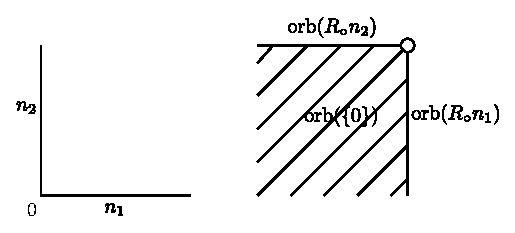
\includegraphics{vol58-fig/fig58-4.eps} 
\end{figure}\pageoriginale


\subsection{}\label{chap1:subsec7.4} \textbf{Projective spaces:}
 The $r$-dimensional projective space $\mathbb{P}_{r}$ is again
 obviously a $(\underbar{k}^{*})^{r}$-embedding. The corresponding
 $(N, \Delta )$ is defined as follows : $N \cong \mathbb{Z}^{r}$ with
 a $\mathbb{Z}$- basis $\{n_{1}, \ldots , n_{r}\}$. Let $n_{0} =
 -(n_{1} + \cdots + n_{r})$. Then $\triangle$ consists of the faces of
 $\sigma_{0}, \ldots , \sigma_{r}$, where 
 $$
 \sigma_{i} = \mathbb{R}_{\circ}n_{0} + \cdots + \overset{i}{\vee} + 
 \cdots + \mathbb{R}_{\circ}n_{r}. 
 $$
\begin{figure}[H]
\centering 
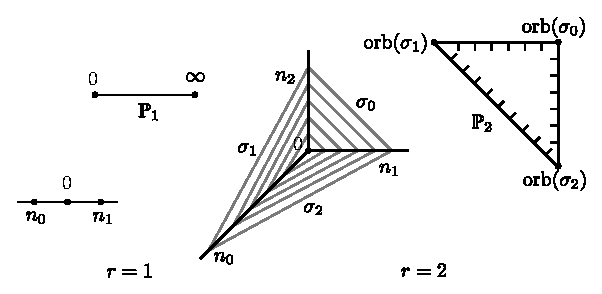
\includegraphics{vol58-fig/fig58-5.eps} 
\end{figure}

 	The canonical morphism $\underbar{k}^{r+1} - \{0\} \to
        \mathbb{P}_{r}$ is equivariant and corresponds to the
        homomorphism $\tilde{N} \cong \tilde{\mathbb{Z}}^{r+1} \to N$
        sending elements of the basis $\{\tilde{n}_{o}, \ldots ,
        \tilde{n}_{r}\}$ of $ \tilde{N}$ to $ \{n_{0}, \ldots ,
        n_{r}\}$.  
 
 	In this connection, we have the following characterization of
        the projective space due to Mabuchi \cite{keyM1}.  

 \begin{theorem}[Mabuchi]\label{chap1:thm7.1} %Throrem 7.1  
 Let $X$ be an $r$-dimensional complete non-singular
   $T$-embedding. Then the following are equivalent.  
\begin{enumerate}[(1)]
\item $X \cong \mathbb{P}_{r}$\pageoriginale equivariantly. 

\item The tangent bundle $\theta_{X}$ of $X$ is ample. 

\item The normal bundle of each $T$-stable irreducible divisor (which
  is non-singular by Theorem \ref{chap1:thm4.3}) is an ample invertible sheaf.  

\item The number of $T$-fixed points of $X$ (which equals the Euler
  number of $X$ by Iversen \cite{keyI6}) is exactly $r + 1$.  

\item The number of $T$-stable irreducible divisors is exactly $r+1$. 

\item Pic $(X) = \mathbb{Z}$.
\end{enumerate}
 \end{theorem} 
 
	 Let $X = T_{N}\emb(\triangle)$. Then (5) means that
         $Sk^{1}(\Delta)$ has $r + 1$ cones. (4) means that $\Delta$
         has $r + 1$ maximal dimensional cones. 
 
 \noindent
 $(1) \Leftrightarrow (4) \Leftrightarrow (5)$ is easy to show in view
 of Proposition \ref{chap1:prop6.7}.  
 
 \noindent
 $(6) \Rightarrow (5) $ follows easily from the exact sequence in
 Proposition \ref{chap1:prop6.1}. 
 
 \noindent
 $(5) \Rightarrow (6)$ follows from the exact sequence and the fact
 that Pix$(X)$ is torsion free. (See Demazure \cite[p.566]{keyD2}).  
 
 \noindent
 $(1) \Rightarrow (2) \Rightarrow (3)$ is well-known. 
 
 \noindent
 $(3) \Rightarrow(4)$ is due to Mabuchi, who showed $(1)
 \Leftrightarrow (2) \Leftrightarrow (3)$ as a special case of
 Hartshorne's conjecture \cite{keyH1} $(H-r)$ to the effect that an
 $r$-dimensional non-singular complete variety with the ample tangent
 bundle is necessarily $\mathbb{P}_{r}$.  
 
 $(H-2)$ is known to be true. $(H-3)$ was proved recently by Mabuchi
 \cite{keyM1} and Mori-Sumihiro \cite{keyMS}. 
 
 \noindent
 $(6) \Rightarrow (1)$ can also be proved directly by means of results
 in Mori \cite{keyM4}, as Sumihiro and Ishida pointed out.  
 
 \subsection{Products}\label{chap1:subsec7.5} % subsection 7.5
 We\pageoriginale leave the proof of the following to the reader. 

 \setcounter{prop}{1}
 \begin{prop}\label{chap1:prop7.2} %Prop 7.2 
Let $(N' , \Delta')$ and $(N'', \Delta'')$ be
r.p.p. decompositions. Then we have  
$$
T_{N'} \emb (\Delta') \times T_{N''} \emb (\Delta'') = T_{N' xN''} \emb
(\Delta' \times \Delta'') 
$$
where $\Delta' \times \Delta''$ is the r.p.p.decomposition of $N'
\times N''$
consisting of cones  
$$
\sigma = \sigma' \times \sigma''
$$
 with $\sigma'$ and $\sigma''$ running through $\Delta'$ and $\Delta''$,
 respectively.  
 \end{prop} 

 
 \subsection{Equivariant fiber bundles}\label{chap1:subsec7.6}
	
 More generally, we have the following description of equivariant
 fiber bundles.  
 
 \begin{prop}\label{chap1:prop7.3} %Prop 7.3
Let $h : (N, \Delta) \to (N' , \Delta')$ be a map of
r.p.p. decompositions, and let $f :X = T_{N} \emb (\Delta) \to X' =
T_{N} \emb (\Delta')$ be the corresponding equivariant dominant
morphism. Consider $N'' = \ker [h : N \to N']$ and an
r.p.p. decomposition $(N'' , \Delta'')$ with $X'' = T_{N''} \emb
(\Delta'')$. Then $f : X \to X'$ is an equivariant fiber bundle with
the typical fiber $X''$ if and only if the following conditions are
satisfied: 
\begin{enumerate}[(i)]
\item $h : N \to N'$ is surjective. 

\item There exists a lifting $\tilde{\Delta'} \subset \Delta$ of
  $\Delta'$, i.e. $(N, \tilde{\triangle'})$ is an
  r.p.p. decomposition and for each $\sigma' \in \triangle'$, there
  exists a unique $\tilde{\sigma'} \in \tilde{\triangle'}$ such that
  $h$ induces a bijection  
$$
h : \tilde{\sigma'} \xrightarrow{\sim} \sigma'.  
$$

\item $\triangle$\pageoriginale consists of the cones 
$$
\sigma = \tilde{\sigma'} + \sigma'' = \{\tilde{y'} + y'' ; \tilde{y'}
\in \tilde{\sigma'}, y'' \in \sigma''\} 
$$
with $\tilde{\sigma'}$ and $\sigma''$ running through
$\tilde{\triangle'}$ and $\triangle''$.  
\end{enumerate}
\end{prop}

	Again we leave the proof to the reader. Note that the lifting
        $\tilde{\triangle'}$ itself defines an open set of $X$ which
        is an equivariant $T_{N''}$-bundle over $X' \cdot X$ is associated
        to it via the $T_{N''}$-action on $X''$.  

\subsection*{($7.6'$)  Equivariant
  $\mathbb{P}_{r}$-bundles:}\label{chap1:subsec7.6'} 
As a special case of (\ref{chap1:subsec7.6}), let $D'_{0}, \ldots , D'_{r}$ be
$T'$-stable Cartier divisors on $X'$ and let $L'_{i} = 0_{X'} 
(D'_{i})$. Then the totally decomposable $\mathbb{P}_{r}$- bundle  
$$
f : X = \mathbb{P} (L'_{0} \oplus \cdots \oplus L'_{r}) \to X' 
$$
has a lifting of $T_{N'}$-action determined by $D'_{i}$'s Moreover,
$X$ has a fiberwise action of $(\underbar{k}^{*})^{r}$ and is a
$T_{N'} \times (\underbar{k}^{*})^{r}$-embedding. A change of Cartier
divisors in the linear equivalence classes gives rise to isomorphic
torus embeddings.  

	In terms of r.p.p.decompositions, it can be described as
        follows: Let $N'' = \mathbb{Z}^{r}$ with a $\mathbb{Z}$- basis
        $\{\ell_{1}, \ldots , \ell_{r}\}$, and let $N = N' \times N''$. For
        each $0 \leq i \leq r$ and $\sigma' \in \triangle'$, there
        exists $m'_{i} (\sigma') \in M' = (N')^{*}$ such that the $A(
        \sigma')$-module $L'_{i}(U(\sigma'))$ is generated by $e
        (m'_{i}(\sigma'))$, by Lemma \ref{chap1:lem6.2}. Let $\ell_{0} = -
        (\ell_{1} + \cdots + \ell_{r}) $, and let $\tilde{\sigma'}$ be
        the image of $\sigma'$ under the linear map $N'_{\mathbb{R}}
        \hookrightarrow N_{\mathbb{R}}$ sending $y'$ to $(y', -
        \sum\limits_{0 \leq i \leq r} \langle m'_{i} (\sigma') , y' \rangle
        \ell_{i})$. 

\noindent
The collection $\tilde{\triangle'} = \{ \tilde{\sigma'} ; \sigma' \in
\Delta'\}$ forms a lifting of $\Delta'$ to
$N_{\mathbb{R}}$.\pageoriginale Then $X =
T_{N} \emb (\triangle)$, where $\triangle$ consists of  
$$
\sigma = \tilde{\sigma'} + \sigma''
$$
with $\tilde{\sigma'}$ running through $\tilde{\triangle'}$ and
$\sigma''$ running through $\triangle'' = \{\text{the faces of }\break
\sigma''_{0} , \ldots, \sigma''_{r}\}$, with $\sigma''_{i} =
\mathbb{R}_{o} \ell_{0} + \cdots + \overset{i}{\vee} + \cdots +
\mathbb{R}_{o}\ell_{r}$.  

\begin{example*}
Let $X' = \mathbb{P}_{1}$ and $r = 1$. For $a \in \mathbb{Z}_{o}$,
consider the rational ruled surface  
$$
X = \mathbb{P} (0_{\mathbb{P}_{1}} \oplus 0_{\mathbb{P}_{1}} (a))
$$
which is usually denoted by $F_{a}$ or $\Sigma_{a}$ and called a
Hirzebruch manifold. The corresponding r.p.p.decomposition of $N=
\mathbb{Z}^{2}$ with a $\mathbb{Z}$- basis $\{n_{1}, n_{2}\}$ looks
like this: 

\begin{figure}[H]
\centering 
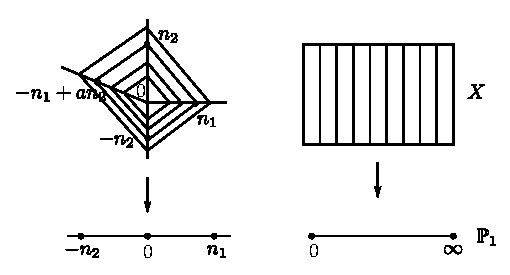
\includegraphics{vol58-fig/fig58-6.eps} 
\end{figure}

\end{example*}

\begin{remark*}
When $E'$ is a $T'$-linearized vector bundle on a $T'$-embedding
$X'$, the bundle $\mathbb{P}(E')$ has a lifting of $T'$-action. But it
is not a torus embedding unless $E'$ is totally decomposable as
above. Nevertheless, it provides us with a typical example of
varieties with torus action which need not be a torus embedding. Thus
it is of some interest to classify equivariant vector bundles on torus
embeddings. This was partly carried out by Kaneyama \cite{keyK1}, who, in
particular, showed the existence of equivariant but not homogeneous
vector bundles on $\mathbb{P}_{2}$. 
\end{remark*}


\subsection{Quotient singularities:}\label{chap1:subsec7.7}
 The quotient singularities explained by\break Mumford et
 all. \cite[p.16-19]{keyTE} fit in nicely with our formulation. 

Let $N \cong \mathbb{Z}^r$ be a free $\mathbb{Z}$-module of rank $r$
with the $\mathbb{Z}$ basis $\{n_1, \ldots, n_r\}$. Let $n'_1, \ldots ,
n'_r \in N$ be primitive elements which are $\mathbb{R}$-linearly
independent in $N_{\mathbb{R}}$, and let $N' \subset N$ be the
$\mathbb{Z}$-submodule of finite index generated by $n'_1, \ldots ,
n'_r$. Consider the simplicial cone  
$$
\sigma= \mathbb{R}_on'_1 + \cdots +\mathbb{R}_on'_r \subset
N_{\mathbb{R}}= N'_{\mathbb{R}}. 
$$

We thus have a map of r.p.p.decompositions $h: (N', \Delta) \to (N,
\Delta)$, where $\Delta$ consists of the faces of $\sigma$. Hence we
have an equivariant surjective morphism 
$$
f: T_{N'} \emb (\Delta)= \underbar{k}^r \longrightarrow X= T_N \emb (\Delta),
$$
which is the quotient map under the canonical action of the
(scheme-theoretic) kernel $\ker[f:T_{N'} \to T_N]$. When the
characteristic of the ground field $k$ does not divide the order of
$N/N'$, then the kernel is (non-canonically) isomorphic to
$N/N'$. Indeed, let $M$ (resp. $M'$) be the  $\mathbb{Z}$-module dual
to $N$ (resp. $N'$). Then $M$ is canonically a submodule of finite
index of $M'$, with a pairing  
$$
\langle ,\rangle:M' \times N \longrightarrow \mathbb{Q}
$$  
which extends the canonical pairings $M \times N \to \mathbb{Z}$ and
$M' \times N \to \mathbb{Z}$, and which, moreover, induces a
non-degenerate pairing   
$$
\langle,\rangle: (M'/M) \times (N/N') \longrightarrow \mathbb{Q}/
\mathbb{Z} 
$$

Then $\ker[f:T_{N'} \to T_N] = \Hom_{gr}(M'/ M, k^*)$, which is
(non-canonically)\pageoriginale isomorphic to $N/N'$ via the above
pairing.   

For instance, let $r=2$. We may choose a $\mathbb{Z}$-basis $\{n_1,
n_2\}$ of $N$ so that  
\begin{align*}
n'_1&=n_1\\
n'_2 &=an_1 +bn_2\\
 \end{align*} 
 where a, $b \in \mathbb{Z}$ with $(a,b)=1$ and $0 \leq a <b$. Then
 the action of $\ker [f:T_{N'} \to T_N]$ on $\underbar{k}^2$ coincides
 with the action  of $\mathbb{Z} /b\mathbb{Z}$ on $\underbar{k}^2$
 with the generator acting via 
 $$
 \underbar{k}^2 \ni (z, w)\longmapsto (\zeta^{-a}z, \zeta w) \in
 \underbar{k}^2, 
 $$
 where $\zeta$ is a primitive $b$-th root of 1 and $z=e(m'_1)$,
 $w=e(m'_2)$ with $\{m'_1, m'_2\}$ the basis of $M'$ dual to $\{n'_1,
 n'_2\}$. 

\begin{figure}[H]
\centering 
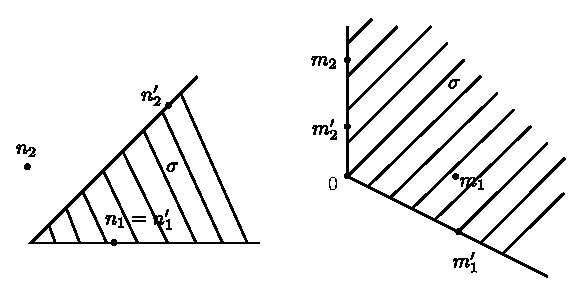
\includegraphics{vol58-fig/fig58-7.eps} 
\end{figure}

 \subsection{Equivariant blowing up:}\label{chap1:subsec7.8}
 
 The maps of the form $h: (N, \Delta'\to (N, \Delta)$ give rise to
 equivariant birational morphisms $f$ of the corresponding torus
 embeddings. Obviously, $f$ is an open immersion  if and only if
 $\Delta' \subset \Delta$. 
 
 The most interesting case is when $\Delta'$ is a \textit{ subdivision
 } of $\Delta$. It was shown by Mumford et all. \cite[Thm.10, p.31]{keyTE}
 that is this case, $f$ is the normalization  of the blowing  up along
 a $T$-stable fractional\pageoriginale ideal. 
 
 They show [ibid., Thm.11, p.32] that given $\Delta$, there always
 exists a subdivision $\Delta'$ which is non-singular, i.e. any torus
 embedding has an \textit{equivariant resolution of singularities }.   
 
 The \textit{minimal resolution} of singularities of a 2-dimensional
 normal torus embedding can be described very simply as in [ibid.,
   p.35-40]. Note that the singularities in this case are isolated,
 and the blowing up an isolated singular point is automatically
 normal, although its description in terms of $r.p.p$. decompositions
 is rather complicated and closely related to continued fractions. In
 this connection, we refer the reader also to Gonzalez-Sprinberg
 \cite{keyG2}, who dealt with \textit{ Nash transforms } of $2$-dimensional
 normal torus embeddings 
 
We need later the following description of a blowing up in the 
 non-singular case. 
 
 \begin{prop}\label{chap1:prop7.4}%% 7.4
Let $T \subset X$ be a non-singular torus embedding corresponding to an
r.p.p.decompositon $(N, \Delta)$. For $\sigma \in \Delta$, the
blowing up of $X$ along the $T$-stable non-singular closed subvariety
$\overline{\orb(\sigma)}$ is a non-singular $T$-embedding
corresponding to the subdivision $(N, \Delta^*)$ obtained from
$\Delta$ by ``starring at its barycenter'' as follows: Let $n_1,
\ldots , n_s$ be the fundamental generators of $\sigma$, and let $n_0
=n_1 + \cdots + n_s$ be the ``barycenter''. For $ \Delta \ni \tau >
\sigma$ and $1 \leq i \leq s$. Let $\tau_i \subset N_R$ be the cone
obtained from $\tau$ by replacing one of its fundamental
generators\pageoriginale $n_i$ by $n_0$ and leaving the other
generators as they are.  
 \end{prop} 
 
\noindent
Then   
$$
\Delta^*=( \Delta- \{\tau \in \Delta; \tau > \sigma\}) \cup(
\bigcup_{\sigma < \tau \in \Delta} \{ \text{ the faces of } \tau_i ;1
\le i \le s \} ). 
$$

 \begin{proof}
$\overline{orb (\sigma)}$ is non-singular by Theorem
   \ref{chap1:thm4.3}. Obviously it 
   is enough to describe the blowing up on the affine open set
   $U(\tau)$ with $U(\tau) \cap \overline{orb(\sigma)} \neq
   \mathbb{Q}$, i.e. $\sigma < \tau \in \Delta$ by Theorem
   \ref{chap1:thm4.2}. Let   $n_1, \ldots, n_s$, with $s \le s'$ be
   the fundamental generators 
   of $\tau$. Since $\tau$ is non-singular, they can be extended to a
   $\mathbb{Z}$-basis $\{n_1, \ldots , n_r\}$ of $N$. Let $\{m_1,
   \ldots , m_r\}$ be the dual basis of $M=N^*$, and let
   $u_i=e(m_i)$. Then the coordinate ring  $A$ of $U(\tau)$ is the
   localization $A=k[u_1, \ldots ,u_r]_{u_{s'+1} \cdots u_r}$ and the
   ideal of $\overline{orb(\sigma)}\cap U (\tau)$ is generated by
   $u_1, \ldots , u_s$. For $1 \leq i \leq s$, let $A_i = A[u_1/u_i,
     \ldots , u_r/u_i]$. Then the inverse image of $U(\sigma)$ in the
   blowing up is covered by Spec $A_i$ with $1 \leq i \leq
   s$. Obviously, Spec $A_i$ is a normal affine $T$-embedding
   corresponding to the cone $\tau_i = \mathbb{R}_o n_0 +
   \sum\limits_{\substack{1 \le j \le s' \\ j \neq i}} \mathbb{R}_o
   n_j$.  
 \end{proof} 

 \setcounter{coro}{4}
 \begin{coro}\label{chap1:coro7.5}%% 7.5
Let $T \subset X$ be a $2$-dimensional non-singular torus embedding
corresponding to an r.p.p.decompostion $(N , \Delta)$. For a
2 dimensional cone $\sigma= \mathbb{R}_o n_1+ \mathbb{R}_on_2$, the
blowing up of $X$ along the $T$-fixed point $ord(\sigma)$ is a
non-singular $T$-embedding corresponding to $(N, \Delta^*)$, where
$\Delta^*$ is obtained from $\Delta$ by removing $\sigma$ and adding
the faces of $\sigma_1 =\mathbb{R}_o(n_1+n_2)+ \mathbb{R}_o n_2$ and
$\sigma_2 = \mathbb{R}_o n_1 + \mathbb{R}_o(n_1 + n_2)$.  
\begin{figure}[H]
\centering 
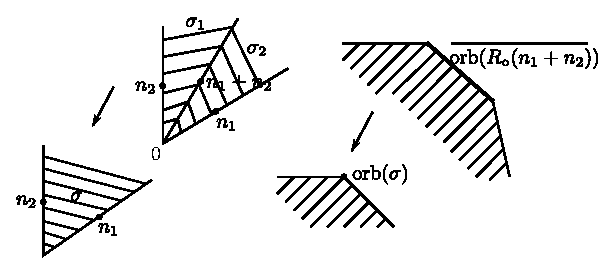
\includegraphics{vol58-fig/fig58-8.eps} 
\end{figure}

 \end{coro}\pageoriginale

 \begin{coro}\label{chap1:coro7.6}%%% 7.6
Let $T \subset X$ be a 3-dimensional non-singular torus embedding
corresponding to an r.p.p.decomposition $(N , \Delta )$. 

\noindent
$(i)$ For a 3-dimensional cone $\sigma= \mathbb{R}_o n_1 +
\mathbb{R}_o n_2+ \mathbb{R}_o n_3$, the blowing up of $X$ along the
$T$-fixed point $\orb(\sigma)$ is a nonsingular $T$-embedding
corresponding to $(N, \Delta^*)$, where $\Delta^*$ is obtained from
$\Delta$ by removing $\sigma$ and adding the faces of $\sigma_1,
\sigma_2$ and $\sigma_3$ as in the picture below. 

\noindent
$(ii)$ For a 2-dimensional cone $\sigma= \mathbb{R}_o n_1 +
\mathbb{R}_o n_2$, let $\tau = \mathbb{R}_o n_1 + \mathbb{R}_o
n_2 +\mathbb{R}_o n_3$ and $\tau'=\mathbb{R}_o n_1+\mathbb{R}_o
n_2+\mathbb{R}_o n_4$ be the $3$-dimensional cones in $\Delta$ having
$\sigma$ as a face (cf. Prop.6.7). Then the blowing up of $X$ along
the $T$-stable curve $\overline{orb(\sigma)}$ is a non singular
$T$-embedding corresponding to $(N, \Delta^*)$, where $\Delta^*$ is
obtained from $\Delta$ by removing $\sigma , \tau, \tau'$ and adding
the faces of $\tau_1, \tau_2, \tau'_1, \tau'_2$ as in the picture
below. 


\begin{figure}[H]
\centering 
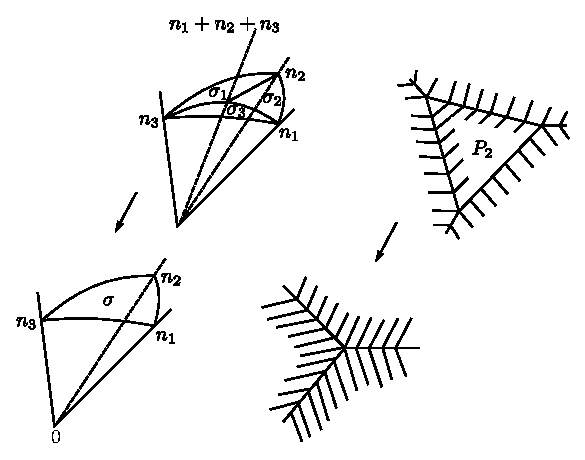
\includegraphics{vol58-fig/fig58-9.eps} 
\end{figure}
\begin{figure}[H]
\centering 
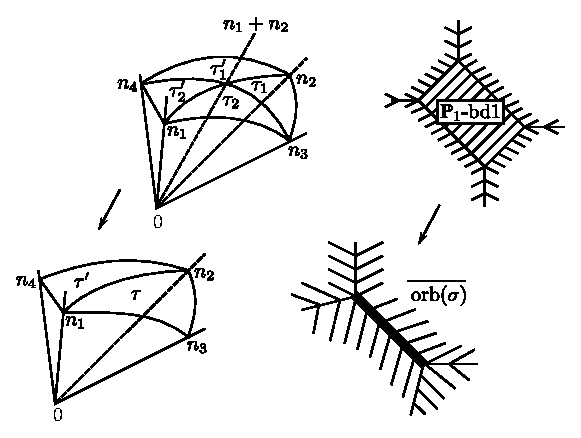
\includegraphics{vol58-fig/fig58-10.eps} 
\end{figure}

 \end{coro}\pageoriginale

 \subsection{Algebraic varieties of monomial type:}\label{chap1:subsec7.9}
 
 As Mumford\pageoriginale et al. \cite{keyTE}\break pointed out in the it
 introduction the theorey  of torus embeddings  is a unified and
 globalized treatment of the ``exponents of monomials''. It can be
 said that when we have algebraic varieties or morphisms defined in
 terms of monomials only, then there is a possibility of formulating
 them more transparently in terms of torus embeddings. We encounter
 many examples in Chapter \ref{chap2}. Here is a motivating example: 
 
 Let $\bar{X} \subset \mathbb{A}_r = \underbar{k}^r$ be a closed
 algebraic set defined polynomials $f_1(t), \ldots , f_\nu (t) \in k
 [t_1, \ldots , t_r]$, each of which is of the form    
 $$
 f(t)= t_1^{a_1} t_2^{a_r} \cdots t_r^{a_r}- t_1^{b_1} t_2^{b_r}
 \cdots t_r^{b_r}  
 $$
 with non-singular integers $a_1, \ldots , a_r, b_1, \ldots ,
 b_r$. Then $\bar{X}$ is invariant the coordinatewise multiplication
 of elements of the group 
 $$
 \bar{T}= \bar{X} \cap (\underbar{k}^*)^r,
 $$
 
 This $\bar{T}$ is an algebraic subgroup of $(\underbar{k}^*)^r$ but
 may not be an algebraic torus. It may neither be connected nor
 reduced. But when $\bar{T}$ is an algebraic torus, then $\bar{X}$  is
 a $\bar{T}$-embedding, although it may not be normal in
 general. Consider, for instance the rational curve with a cusp 
 $$
 \bar{X}= \{(t_1, t_2) \in \mathbb{A}_2 ; t_2^2 =t_1 ^3\}.
 $$ 
 We have analogues in $\mathbb{P}_r$ or its generalization in Mori \cite{keyM3}
 
 Here is\pageoriginale a more general formulation in the  affine case
 Let $M \cong  \mathbb{Z}^r$ and let $0 \in  S$ be a finitely
 generated sub  semigroup of $M$ which generates $M$ as a group. Hence   
 $$
 X=\Hom_{\text{u.s.g}}(S,\underbar{k})
 $$  
 is a $T$-embedding with 
 $$
 T=\Hom_{gr}(M, \underbar{k}^*). 
 $$

 Let $m_1, \ldots , m_\nu , m'_1 , \ldots , m'_\nu \in S $. Then
 consider the quotient 
 
  $\bar{M} = M/$ (the subgroup  $gen^{\underbar{d}}$ by $m_1- m'_1 ,
 \ldots , m_\nu - m'_\nu$) and the image  $\bar{S}$ of $S$ under the
 canonical projection $M \to \bar{M}$. Then  $\bar{S}$ is the
 quotient of $S$ with respect to the equivalent relation  
 $$
 s \sim s' \Leftrightarrow {^\exists} s'' \in S, a_1, \ldots , 
 a_\nu, b_1, \ldots ,b_\nu  \in \mathbb{Z}_o \text{ such that } 
 $$
 \begin{align*}
s &=s'' + \Sigma a_i m_i + \Sigma b_i m'_i\\
s'&=s'' + \Sigma b_i m_i + \Sigma a_i m'_i
 \end{align*} 

 Let 
 \begin{align*}
\bar{T}&=\Hom_{gr}( \bar{M}, \underbar{k}^*) \subset T \quad\text{
  algebraic subgroup}\\ 
\bar{X}&= \Hom_{u.s.g}(\bar{S}, \underbar{k}) \subset X \quad\text{
  closed algebraic set}. 
 \end{align*} 
 
 Then $\bar{X}$ contains $\bar{T}$ as a dense open  subset and is
 invariant under $\bar{T}$. If $m_1- m'_1, \ldots , m_\nu - m'_\nu$
 generates a pure subgroup of $M$, then $\bar{T}$ is an algebraic
 torus and $\bar{X}$ is a $\bar{T}$-embedding. If, moreover, $S=
 \check{\sigma} \cap M$ for a cone $\sigma \subset N_{\mathbb{R}}$ as
 in (\ref{chap1:subsec5.1}), then the \textit{ normalization } of $\bar{X}$
 corresponds to the cone $\sigma \cap \bar{N}_\mathbb{R}$, where
 $\bar{N}= N \cap \{m_1-m'_1, \ldots , m_\nu- m'_\nu \}^\perp$.
 
 \section{Torus embeddings of dimension $\le 2$}\label{chap1:sec8}
 
 It\pageoriginale is easy to see that 1-dimensional normal torus
 embeddings are 
 $\underbar{k}^*, \mathbb{A}_1 = \underbar{k}$ and $\mathbb{P}_1$, up
 to isomorphism.  
 
 \medskip
 From  now in this section, Let $N \cong \mathbb{Z}^2$ and $T=T_N$. A
 2-dimensional normal $T$-embedding of finite type looks like this:  
\begin{figure}[H]
\centering 
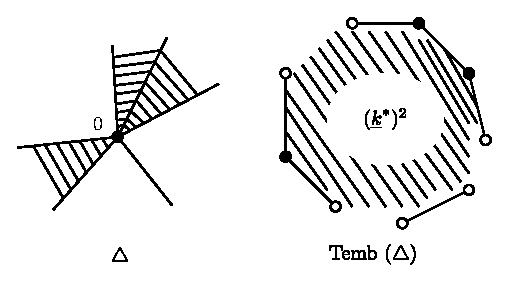
\includegraphics{vol58-fig/fig58-11.eps} 
\end{figure}

  
  In particular, a complete normal $2$ dimensional $T$-embedding is
  determine by a finite cycle of primitive elements  $n_1, \ldots, n_d$
  in $N$ going counterclockwise once around $0$ in the given order
  such that det $(n_i,\break n_{i+1})> 0$ for $1 \leq i \leq d$
  $(n_{d+1}=n_1)$, i.e. $n_{i+1}$ lies strictly before  $-n_i$ (which
  may not belong to the cycle). 
\begin{figure}[H]
\centering 
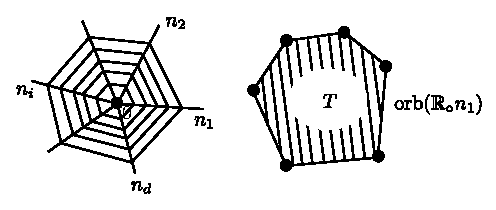
\includegraphics{vol58-fig/fig58-12.eps} 
\end{figure}

  
  \begin{prop}\label{chap1:prop8.1} %% 8.1
Any\pageoriginale 2-dimensional normal torus embedding $T \subset X$
of finite is quasi-projective, i.e. can be equivariantly embedded into
a projective space.  
  \end{prop} 

  \begin{proof}
Let $X=$ Temb $(\Delta)$. By filling in the complement
$N_{\mathbb{R}}- \bigcup\limits_{\sigma \in \Delta} \sigma$ by
appropriate cones if necessary, we can embed $X$ equivariantly into a
complete normal $T$-embedding. (For the existence of equivariant
completions in general, we refer the reader to Sumihiro \cite{keyS3}.) We
may thus assume that $X$ itself is complete. Let $n_1, \ldots n_d$ be
the fundamental generators of the $1$-dimensional cones in $\Delta$
arranged, as above, in such a way that they go around $0$
counterclockwise once in this order. By Theorem \ref{chap1:thm6.4},
$X$ is projective 
if and only if there exist $a_1, \ldots , a_d \in \mathbb{Z}$ such
that for each 2-dimensional cone $\sigma \in \Delta $, there exists
a unique $m(\sigma) \in M$ with $\langle (\sigma), n_i \rangle \geq
-a_i$ ~$1 \leq i \leq d$ and with the equality holding if and any if
$n_i \in \sigma$. As we remarked after the proof of Theorem \ref{chap1:thm6.4},
this means that the convex hull of    
$$
\{ M(\sigma): \Delta \ni \sigma  ~~\text{2-dimensional}\} 
$$
in $M_\mathbb{R}$ has exactly $d$ edges $F_1, \ldots , F_d$ going
around 0 in this order with $F_i$ perpendicular to $n_i$. 
   \end{proof}   
   
   It is thus enough to show, by induction on $d$, the existence of a
   convex polygon $P$ in $M_\mathbb{R}$ with the vertices in
   $M_\mathbb{Q}$ such that it has exactly $d$ edges $F_1, \ldots ,
   F_d$ going around 0 in this order with $F_i$ perpendicular to
   $n_i$ 
   
   Obviously\pageoriginale $d \geq 3$ and the case $d=3$ is
   trivial. If $d \geq 4$, 
   there certainly exists $n_d$, say, such that the cycle $n_1, \ldots
   , n_{d-1}$ still defines an $f.r.p.p$. decomposition. Let $P'$ be a
   polygon with $d-1$ edges $F'_1, \ldots , F'_{d-1}$ satisfying the
   required property. At the vertex of $P'$ which is the intersection
   of edges $F'_1$ and $F'_{d-1}$, we can cut the corner by a line
   perpendicular to $n_d$ and obtain a required $P$ with $d$ edges. 
\begin{figure}[H]
\centering 
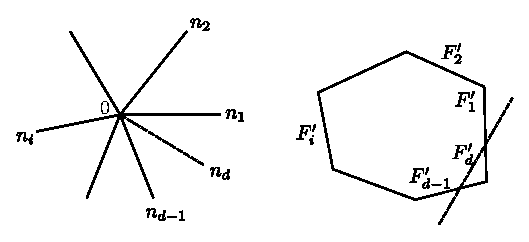
\includegraphics{vol58-fig/fig58-13.eps} 
\end{figure}

   A complete non-singular 2-dimensional $T$-embedding is determined
   by a cycle of elements $n_1, \ldots , n_d \in N$ as above with  
   $$
   \det(n_i, n_{i+1}) =1 \quad 1 \le i \le d. 
   $$ 
   This condition is rigid enough to allow a complete classification. 

\setcounter{theorem}{1}   
   \begin{theorem}\label{chap1:thm8.2}%%% 8.2
Up to isomorphism, a complete non-singular $2$ - dimensional
$T$-embedding is obtained from  
$$
\mathbb{P}_2  \text{ or } F_a = \mathbb{P}(0_{\mathbb{P}_1} \oplus
0_{\mathbb{P}_1} (a)) \qquad 1 \neq a \geq 0 
$$
by a finite succession of blowing ups along $T$-fixed points. It can
be transformed to $\mathbb{P}_2$ by a finite succession of blowing ups
and\pageoriginale blowing downs along $T$-fixed points. Given non-singular
$T$-embeddings $X$ and $X'$, there exists $X''$ obtained both from $X$
and from $X'$ by a finite succession of blowing ups along $T$-fixed
points. 
   \end{theorem}   
 
   \begin{proof}
Let $X=$Temb $(\Delta)$ with $\Delta$ determined by a cycle $n_1,
\ldots , n_d \in N$ going around 0 once counterclockwise. Certainly
$d \geq 3$. If $d=3$, then  $n_1 +n_2+n_3=0$ and $X=\mathbb{P}_2$
(cf. Theorem \ref{chap1:thm7.1}). We may thus assume $d \geq 4$. 
   \end{proof}  

\setcounter{lemma}{2}    
  \begin{lemma}\label{chap1:lem8.3}
If $d \geq 4$, there exist $i$ and $j$ with $n_i + n_j=0$.  
  \end{lemma}  

\setcounter{sublemma}{3}  
  \begin{sublemma}\label{chap1:sublem8.4}%% 8.4
Let $\{n, n'\}$ and $\{\ell, \ell'\}$ be $\mathbb{Z}$-bases of $N$. If
$\ell$  lies in the interior of the sector $\mathbb{R}_o n+
\mathbb{R}_o n'$ and if $\ell'$ is in the sector $\mathbb{R}_o n'+
\mathbb{R}_o (-n)$, then $\ell' =n'$ or $\ell' =-n$. 

\begin{figure}[H]
\centering 
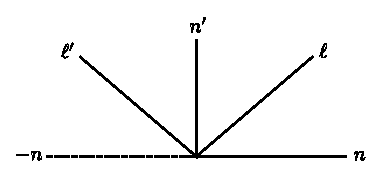
\includegraphics{vol58-fig/fig58-14.eps} 
\end{figure}
  \end{sublemma}  
  

\medskip
\noindent{\textbf{Proof of the sublemma:}}
By assumption, there exist positive integers $a, a'$ such that $\ell =
an +a'n'$ and non-negative integers $b,b'$  such that  $\ell'=-
bn+b'n'$. We are done, since $1= \det(\ell, \ell')=ab'+a'b$ by
assumption.  

\medskip
\noindent{\textbf{Proof of the lemma:}}
Suppose the assertion  of the lemma is false. By re-numbering the
primitive elements if necessary, we may assume that starting
counterclockwise from $n_1$, we have more than half  
of the\pageoriginale primitive elements before $-n_1$, which does not
coincide with 
any of the $n_i 's$ by assumption. Let $n_j (j>2)$ be th last
primitive element before $-n_1$. Since  $n_{j+1}$ does not coincide
with $-n_1$ and $-n_2$, we see by sublemma \ref{chap1:sublem8.4} and the  convexity
that $n_{j+1}$ is  is strictly between  $-n_2$ and $-n_j$. Thus  we
conclude that $n_2, n_3, \ldots , n_j$ and  $-n_{j+1}$, $-n_{j+2}, \ldots
  , -n_d, -n_1$ are all  different and lie between $n_2$ and $-n_1$. 

\begin{figure}[H]
\centering 
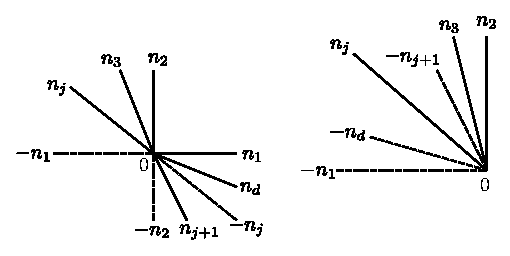
\includegraphics{vol58-fig/fig58-15.eps} 
\end{figure}


\noindent
This is obviously a contradiction in view of  Sublemma \ref{chap1:sublem8.4}. 

\medskip\noindent
\textbf{Proof of Theorem 8.2 continued:} By Lemma \ref{chap1:lem8.3}, we may
assume that $n_d +n_i = 0 $ for some $i$. Let $n' = -n_d = n_i$ and $n
= n_1$. Thus $\{ n,n'\}$ is a basis of $N$. 

If  $d= 4$, we see that $n_2 = n'$ and $n_3 = -n + an'$ for some
integer a. This  gives rise to $X = F_a$. By symmetry, we may assume
that $a \geq 0$. If $a = 1, n'$ is the sum of the adjacent  primitive
elements, hence by blowing down  we  can eliminate $n'$.  

Thus we may assume $d \geq 5$ and at least one  primitive element lies
between $n=n_1$ and $n' = n_i$. It remains to show that  
\begin{figure}[H]
\centering 
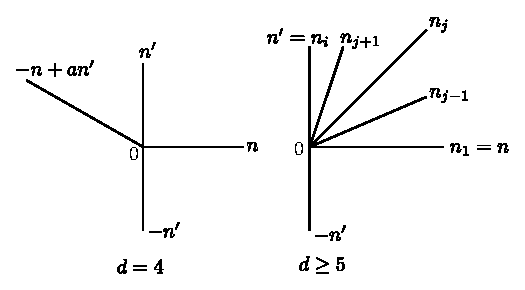
\includegraphics{vol58-fig/fig58-16.eps} 
\end{figure}\pageoriginale
there exists $1<j<i$ such that $n_j = n_{j-1} + n_{j+1}$. For each $1
\leq j \leq i$, there exist non -negative integers  $b_j,b'_j$ with
$n_j = b_jn +b'_jn$. On the other hand for each $j$, there exists an
integer $a_j$ such that $n_{j-1} + n_{j+1} + a_j n_j = 0 $ by
Proposition \ref{chap1:prop6.7}. Obviously $a_j < 0$. Consider the  function  
$$
c(j) = b_j + b'_j > 0.
$$

Then  $ c(j-1) + c(j+1) + a_jc(j) = 0 $. Moreover, since $c (1) = c(i)
= 1$, there exists $j$ so that  $c (j)>c(j+1)$ and $c (j)\geq
c(j-1)$. For this  $j$, we have   $(2 +a_j) c (j) >0$ and conclude
$a_j = -1$. This means that if  $d \geq 5$, we can successively blow
$X$ down to some $F_a$. (cf. the Farey series in additive number
theory.)  

This  fact can  also be proved sing Nagata's classification  \cite{keyN1}
of relatively minimal models of rational surfaces. Note that an
exceptional curve of the first kind is automatically  $T$-stable,
hence the blowing down is equivariant. 

As for the  second assertion  of Theorem \ref{chap1:thm8.2}, we may assume  $X =
F_a$. If we insert the sum of  $-n +an'$ and  $-n'$ between them, then
$-n +an'$  is the sum of  $-n + (a-1)n'$ and  $n'$. 
\begin{figure}[H]
\centering 
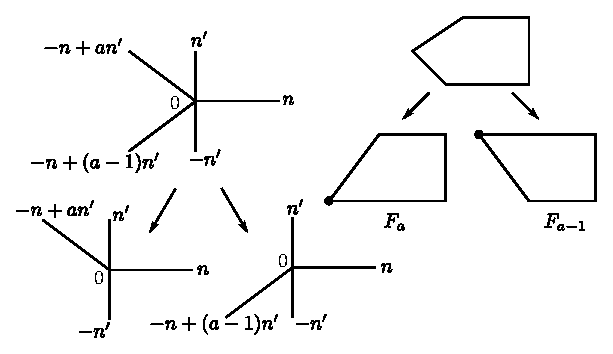
\includegraphics{vol58-fig/fig58-17.eps} 
\end{figure}


This\pageoriginale means that by blowing up a long a  $T$-fixed point
of $F_a$ and 
then blowing down a $T$-stable  curve, we get $F_{a-1}$. This  process
is usually called an \textit{elementary transformation} of a ruled
surface. By a finite repetition of this process, we transform  $F_a$
to $F_1$, which can be blown  down to $\mathbb{P}_2$. 

The  last assertion of Theorem \ref{chap1:thm8.2} follows  easily from the
decomposability of birational morphisms of non-singular surfaces
into blowing ups along closed points. But it can also be proved in
terms of r.p.p.decompositions as follows: Let $X =$ Temb $(\Delta)$
and  $X' = $ Temb $(\Delta') $. Then the decomposition of $N_R$ 
obtained by the  intersections  $\sigma \cap \sigma'$ with $\sigma \in
\Delta$ and $\sigma' \in \Delta$ need not be non singular, but  it has
a non singular subdivision $\Delta''$. Thus it is enough to show  that
a non singular subdivision $\Delta''$ of a non-singular $\Delta$ is
obtained by  finite succession of operations in  Corollary
\ref{chap1:coro7.5}. This 
can be seen exactly as in the last part of the proof of the first
assertion. 

Let us\pageoriginale now derive certain consequences from Theorem
\ref{chap1:thm8.2} which we need in the next section and which are also of
independent interest.  

Let a cycle  $n_1, \ldots , n_d$ of primitive elements in $N$
determine a complete non-singular $2$- dimensional torus embedding $X
= $Temb $(\Delta)$. Let $D_i = \overline{\orb (\mathbb{R}_o n_i)}$. Then by
Proposition \ref{chap1:prop6.7}, we have   
$$
n_{i-1} +n_{i+1} + a_i n_i = 0 \quad 1 \leq i \leq d 
$$
and 
$$
a_i = D^2_i.
$$
Thus we have a cycle $D_1, \ldots , D_d$ of non-singular rational
curves, which can be expressed, as usual, by a circular graph with
weights  $a_i$. Note that this weighted circular graph determines the
2-dimensional $T$-embedding $X$ up to isomorphism. 
\begin{figure}[H]
\centering 
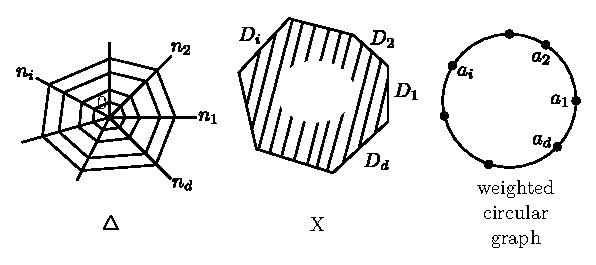
\includegraphics{vol58-fig/fig58-18.eps} 
\end{figure}


The cycle $a_1, \ldots , a_d$ of integers cannot be arbitrary. For
instance, we have the following necessary but not sufficient condition
as a consequence of Noether's formula $K^2 + c_2 = 12$ and  $c_2
=d$\pageoriginale (cf. Iversen[I6]):   
$$
a_1 + \cdots + a_d = 3 (4-d).
$$
We have the following characterization as a consequence of Theorem
\ref{chap1:thm8.2}. 

\setcounter{coro}{4}
\begin{coro}\label{chap1:coro8.5}%% 8.5
A weighted circular graph with  $d$ vertices corresponds to a
2-dimensional complete non-singular torus embedding if  and only if
it is  obtained from those with $d=3$ or $d=4$ below by a successive
application of the  following  operation: insert  one  vertex with
weight $-1$ and subtract 1 from the  weights of the two adjacent
vertices. For $d \leq 6$, we have the following possible cases. 
\end{coro}
\begin{figure}[H]
\centering 
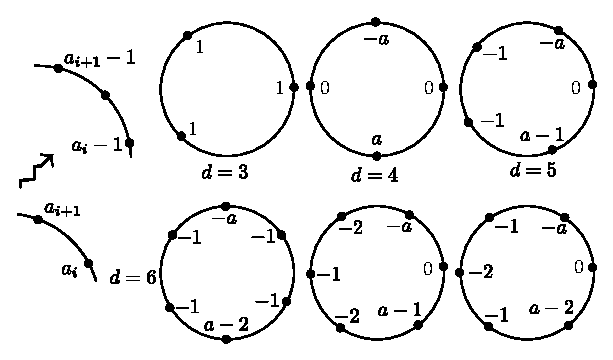
\includegraphics{vol58-fig/fig58-19.eps} 
\end{figure}\pageoriginale


\begin{remark*}
 A 2-dimensional complete non-singular torus embedding can be
  considered as a compactification of $\underline{k}^2$, the affine
  plane, in many different ways. The graph obtained  from the
  corresponding wighted circular graph by removing two adjacent
  vertices is the graph of the complement of
  $\underline{k}^2$. cf. Morrow \cite{keyM6}. 
\end{remark*}

\section{Complete  non-singular torus embeddings in dimension
  3}\label{chap1:sec9}

In\pageoriginale this section, we give a partial classification of
$3$-dimensional 
complete non-singular torus embeddings. As by-products we get many
non-projective  complete non singular threefolds and  birational
morphisms which cannot be written as a succession of  blowing ups
along non-singular centers. These are  of some independent interest
even if the torus action is ignored. 

Torus embeddings provides us  with a good testing ground for the
birational geometry of non-singular varieties, since many questions
are reduced to the  elementary geometry of
r.p.p.decompositions. Consider, for instance, the following basic
question. By abuse of language, a blowing up $Y \rightarrow X$ along a
non-singular center of $X$ is also called a \textit{blowing down of}
$Y$ \textit{along a non-singular center}.  

\medskip
\noindent
{\bf Question:} Let $X$ and $X'$ be birational non-singular algebraic
varieties. 

\medskip
\noindent
\textbf{(strong version)} Does there exist $X''$ which can be obtained
both from $X$ and from $X'$ by a finite succession of blowing ups
along non-singular centers? 

\medskip
\noindent
\textbf{(weak version)} Can $X'$ be obtained from $X$ by a finite
succession of blowing ups and blowing  along non-singular centers? 

The answer is affirmative dimension 2, but is not known
even\pageoriginale in dimension 3. According to Hironaka \cite{keyH3}, we
have the  following weaker affirmative answer in characteristic 0:
There exists $X''$ obtained from $X$ by a finite succession of blowing
ups along non-singular centers such that there exists  a
\textit{morphism} from $X''$ to $X'$.  
 
In the case  of torus embeddings, the question is completely reduced
to one on non-singular r.p.p.decompositions  and looks much
easier.\break Nevertheless, we were  unable to prove the following
conjecture even in dimension 3. We have already shown  in Theorem
\ref{chap1:thm8.2} that the conjecture is true in dimension 2. 

\medskip
\noindent
\textbf{Conjecture}

\medskip
\noindent
\textbf{(strong version)} Let $X$ and $X'$ be non-singular
$T$-embeddings. Then there exists a $T$-embedding $X''$ obtained both
from $X$ and  from $X'$ by a finite succession of $T$-equivariant
blowing ups along $T$-stable non-singular centers. 

\medskip
\noindent
\textbf{(weak version)} Any complete non-singular $r$-dimensional
torus embedding is  obtained from $\mathbb{P}_r$ by a finite
succession of equivariant blowing ups and blowing downs along
non-singular centers. 

From now on, we fix $N \cong \mathbb{Z}^3$ and the ground field
$k$. \\
Let  $T = T_N$. 

The classification of 3-dimensional complete non-singular
$T$ - embeddings $X$ is reduced to that  of f.r.p.p.decompositions
$\Delta$ of $N_\mathbb{R} \cong \mathbb{R}^3$ such that $N_\mathbb{R}
= \bigcup \limits_{\sigma \in \Delta} \sigma$ and that the fundamental
generators of each  3-dimensional $\sigma \in \Delta$ form  a
$\mathbb{Z}$-basis of $N$. 

It is\pageoriginale slightly more complicated to describe such
$\Delta$ in a computable way than in the 2-dimensional case.  

\begin{defi*}
Let $S = S^2$ be a sphere in $N_\mathbb{R}$ centered at 0. Consider
a triangulation of $S$ by spherical triangles. 
\end{defi*}

\noindent
$(i)$ By an $N-$\textit{weighting} of the triangulation. we mean a
primitive element of $N$ attached to each spherical vertex. 

\noindent
$(ii)$ By a \textit{double} $\mathbb{Z}-$\textit{weighting} of the
triangulation, we mean a pair of integers attached to each spherical
edge with one integer on the side of one vertex and with the other on
the  side of the other vertex. Let $v_1, \ldots , v_s$ be the
vertices adjacent to a vertex $v$ of the triangulation, and let $a_i$
be the $\mathbb{Z}$-weight on the edge $vv_i$ which is on the side of
$v_i$. The \textit{weighted link} of $v$ is the spherical polygon
$v_1v_2\cdots v_s v_1$ together  with weights $a_i $ at $v_i$. 
\begin{figure}[H]
\centering 
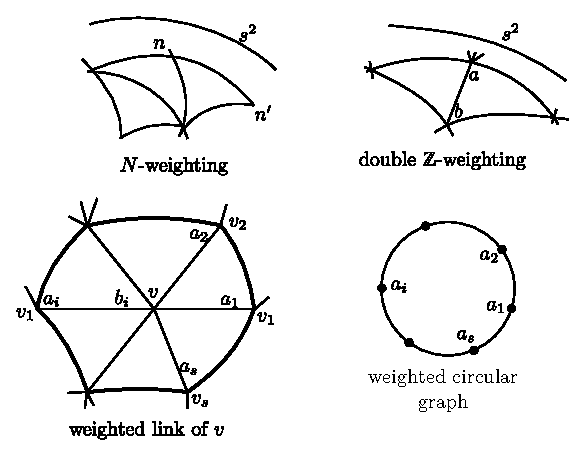
\includegraphics{vol58-fig/fig58-20.eps} 
\end{figure}

Let\pageoriginale $X =$ Temb $(\Delta)$ be a  3-dimensional complete
non-singular torus embedding. If we intersect $\Delta$ with a sphere
$S \subset N_R$ centered at 0, we get a triangulation of $S$  
$$
S = \bigcup_{\sigma \in \Delta} (\sigma \cap S).
$$
We have a canonical $N$-weighting for this triangulation. Indeed, each
spherical vertex is of the form 
$$
(\mathbb{R}_\circ n)\cap S
$$
for a primitive $n \in N$, which we attach to the vertex. Obviously,
$\Delta$ is determined completely by this $N$-weighted triangulation of
$S$. 

\begin{defi*}
An $N$-weighted triangulation of $S^2$ is \textit{admissible} if it is
obtained from a complete non-singular $X = $ Temb $ (\Delta)$ in this
way. 
\end{defi*}

The admissibility means the following : For each spherical triangle,
the $N$-weights $\{n,n',n''\}$ at the three vertices from a
$\mathbb{Z}$-basis of $N$ and the cone $\mathbb{R}_\circ n +
\mathbb{R}_\circ n' + \mathbb{R}_\circ n''$ cuts  out
the original triangle on $S$. 

On the other hand, an admissible $N$-weighting for a triangulation of
$S$ gives rise to a double $\mathbb{Z}$-weighting. Indeed, each
spherical edge is of the form 
$$
\tau \cap S
$$
for a 2-dimensional cone $\tau \in \Delta$. Let $\{n_1, n_2\}$ be
the fundamental generators of $\tau$. By Proposition
\ref{chap1:prop6.7}, $\tau$ is 
the common fact of\pageoriginale exactly two 3-dimensional cones
$\sigma$ and $\sigma'$. Let  $\{n,n_1, n_2\}$ and  $\{n',n_1, n_2\}$
be the fundamental generators of $\sigma$ and $\sigma'$,
respectively. There exist $a, b\in \mathbb{Z}$ such that   
$$
(*) n+n' +an_1 +bn_2 = 0.
$$
We attach a pair  $(a,b)$ to the edge  $\tau \cap S$, with a on the
side of $(\mathbb{R}_on_1) \cap S$ and $b$ on the side of
$(\mathbb{R}_on_2)\cap S$.  
\begin{figure}[H]
\centering 
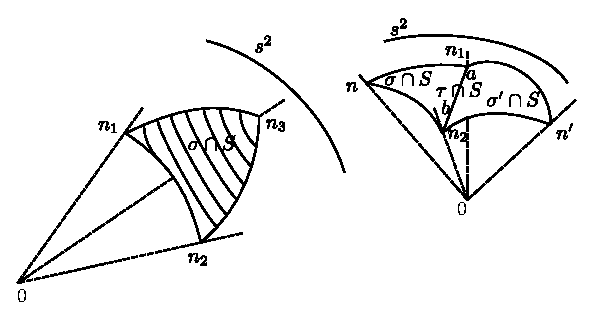
\includegraphics{vol58-fig/fig58-21.eps} 
\end{figure}


 In this  case, consider a vertex $v$ with $N$-weight $n$
 and  its link with the vertices $v_1, \ldots , v_s$ with $N$-weights
 $n_1, \ldots , n_s$ going  around $v$ in this order. Let $D =
 \overline{\orb (\mathbb{R}_on)}$ and $D_i = \overline{\orb
   (\mathbb{R}_on_i)} ~ ~ 1\leq i  \leq s $ be the corresponding
 $T$-stable irreducible divisors on $X = 
 $ Temb $(\Delta)$. Again by Proposition \ref{chap1:prop6.7}, we have 
 $$
 (**) n_{i-1} + n_{i+1} + a_in_i +b_in = 0 \quad 1 \leq i \leq s, 
 $$
 where $n_0 = n_s$, $n_{s+1} = n_1$, and 
$$
a_i = D^2_i \cdot D.
$$
 
 \noindent
 Since $D$ is  a 2-dimensional complete non-singular torus
 embedding\pageoriginale (cf. Theorem \ref{chap1:thm4.3}) with stable curves $D_i
 \cap D$  $1 \leq i \leq s$, we see that the weighted link at $v$ is
 exactly the weighted circular graph of $D$ described immediately
 before Coro \ref{chap1:coro8.5}.  
\begin{figure}[H]
\centering 
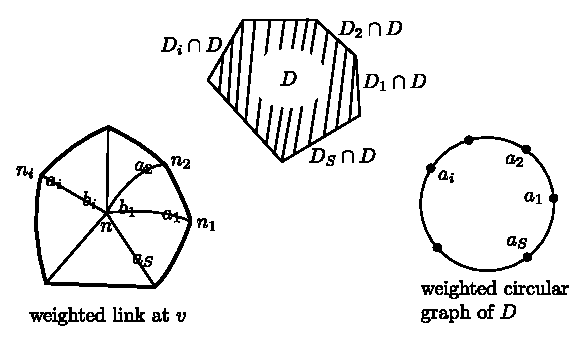
\includegraphics{vol58-fig/fig58-22.eps} 
\end{figure}
 
 \begin{defi*}
A doubly $\mathbb{Z}$-weighted triangulation of $S^2$ is called
\textit{admissible} if, around each vertex, the equations $(**) 1 \leq
i \leq s$ in unknowns  $n, n_1 ,\ldots , n_s$ are compatible and if,
moreover, the weighted link of \textit{each} vertex is a weighted
circular graph obtained as in Corollary \ref{chap1:coro8.5}. 
 \end{defi*} 

\begin{defi*}
An isomorphism from an admissible $N$-weighted triangulation to
another is  an  automorphism of $N$ which induces an isomorphism
from the corresponding f.r.p.p.decomposition to another. $A$
\textit{combinatorial isomorphism} from an admissible doubly
$\mathbb{Z}$- weighted triangulation of $S^2$ to another is an
incidence and $\mathbb{Z}$-weight preserving bijection from the set of
spherical simplices of one triangulation to that of the other. 
\end{defi*}

\begin{prop}\label{chap1:prop9.1}%% 9.1
We have\pageoriginale canonical bijections
$$
\left \{\begin{minipage}{2.7cm}
{isom. classes of $3-\dim \underbar{1}$
  complete n.s. torus embeddings/k } 
\end{minipage} \right\}
\xrightarrow{\sim}
\left\{\begin{minipage}{2.5cm}
{isom. classes of admissible N-weighted triang$\underbar{ns}$ of
  s}
 \end{minipage}\right\} 
 \xrightarrow{\sim}\left
\{\begin{minipage}{3cm}
 {combinatorial isom. Classes of admissible
    doubly $\mathbb{Z}$-wei-ted triang$\underbar{ns}$ of S}
\end{minipage}\right \} 
$$
\end{prop}

\begin{proof}
From what we have seen so far, it is enough to prove the surjectivity
of the second map. Let $\{n,n',n''\}$ be a $\mathbb{Z}$ -basis  of
$N$. Pick an arbitrary triangle of an admissible doubly
$\mathbb{Z}$-weighted triangulation of $S$, and give $N$-weights
$n,n',n''$  to its three vertices in any way. Then using the
equality $(*)$, we can successively determine the $N$-weights of the
other vertices of the  triangulation. This $N$-weighting  is
admissible. Indeed, for each vertex $v$ with $N$-weight $n$, the
vertices  $v_1 , \ldots , v_s$  with $N$-weights $n_1 , \ldots , n_s$
of its link satisfy the equalities  $(**)$. Since the double
$\mathbb{Z}$-weighting  is admissible, $n_1 , \ldots , n_s$ go  around
$n$ \textit{once} in this order, by Proposition \ref{chap1:prop6.7} applied to
$N/\mathbb{Z}n$ and the images in it of  $n_1 , \ldots , n_s$. Thus
the spherical triangles on $S$ cut out  by  
$$
\mathbb{R}_\circ n + \mathbb{R}_\circ n_i + \mathbb{R}_\circ n_{i+1}
\quad  1\leq i \leq s  
$$
together fill up a neighborhood of $(\mathbb{R}_\circ n)\cap S$ combinatorially
isomorphic to the  star of $v$ in the original triangulation which is
the spherical  polygon with vertices  $v_1 , \ldots , v_s$. Since $S$
is simply connected, we are done. 
\end{proof}

\begin{remark*}
The\pageoriginale advantage of using admissible double
$\mathbb{Z}$-weighting is  
the following: Once a combinatorial type of a triangulation of $S^2$
is given, possible admissible double $\mathbb{Z}$-weighting on it are
computable in principle, although it is more convenient sometimes to
use information's on the N-weights. To state the final result, however,
it is less cumbersome to choose a convenient $\mathbb{Z}$-basis of $N$
and describe one possible admissible N-weighting corresponding to it
in terms of the $\mathbb{Z}$-basis.  
\end{remark*}

\noindent
\textbf{Convention} Given an admissible N-weighted triangulation of
$S$ and a vertex with the N-weight $n$, we call that vertex {\em{the
    vertex $n$}}, for simplicity, although $n$ itself need not be on
$S$. 


By Corollary \ref{chap1:coro7.6}, the blowing up of $X=Temb (\Delta)$ along
$\overline{orb(\sigma)}$ corresponds to the following subdivision of
the $N$-weighted triangulation $\underset{\tau\in
  \triangle}{\bigcup}(\tauup \cap S)$. 
\begin{figure}[H]
\centering 
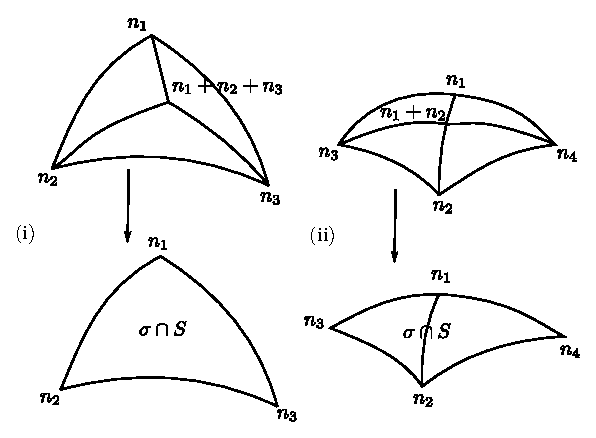
\includegraphics{vol58-fig/fig58-23.eps} 
\end{figure}
 
The following\pageoriginale result, whose proof is immediate, will
turn out to be useful in our classification below.  

\setcounter{coro}{1}
\begin{coro}\label{chap1:coro9.2}%%%% 9.2
Given an admissible $N$-weighted triangulation of $S=S^2$, let $n$ be
a vertex and let $n_1,\ldots, n_2$ be the vertices of its link going 
around $n$ in this order. 
\end{coro}

\begin{enumerate}[(i)]
\item If $ s \ge 4$, there exist $i,j$ such that the vertices $n_i, n,
  n_j$ are collinear on $S$, i.e are on a great circle. 

\item If the vertex $n$ is \textit{3-valent}, i.e. $s=3$, there
  exists an integer $b$ such that $n_1 + n_2 + n_3 + bn=0$. The vertex
  $n$ can be eliminated by a blowing down along a non-singular center
  if and only if $b=-1$. The double $\mathbb{Z}$-weights around the
  vertex $n$ are as in the picture below.    

\item If the vertex $n$ is \textit{4-valent}, i.e $s=4$, there exist
  integer $a,b,c$ such that after re-numbering $n_i$'s, we have $n_2 +
  n_4 + bn = 0$ (in particular, the vertices $n_2, n, n_4$ are
  collinear) and $n_1 + n_3 + an_2 + cn =0$. The vertex $n$ can be
  eliminated by a blowing down along a non-singular center if and only
  if $b=-1$. The double $\mathbb{Z}$-weights  around the vertex $n$
  are as in the picture below. 

\item If the vertex $n$ is \textit{5-valent}, i.e. $s=5$, there
  exist integer $a, b_1, b_2, b_3,\break b_4, b_5$ with $b_1 = b_3 + b_4$
  and $(-1)b_2 + (a-1)b_3 = (-a)b_4 + (-1)b_5$ such that, after
  re-numbering $n_i$'s we have $n_1 + n_3 + (a-1)n_2 + b_2n = 0; n_2 +
  n_4 - n_3 + b_3n = 0 , n_3 + n_5 - n_4 + b_4n = 0, n_4 + n_1- an_5 +
  b_5n = 0$ and\pageoriginale $n_2 + n_5 + b_1n=0$ (in particular, the
  vertices $n_2,   n, n_5$ are collinear) The double
  $\mathbb{Z}$-weights around the vertex $n$ are as in picture below.  
\begin{figure}[H]
\centering 
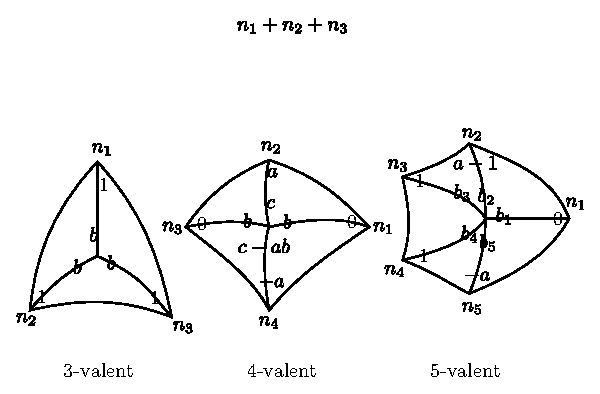
\includegraphics{vol58-fig/fig58-24.eps} 
\end{figure}

\end{enumerate}

To show that a given complete non-singular $ X = Temb(\Delta)$ is
projective, i.e. there exist integers $a_i$ satisfying the condition
$(iii)$ of Corollary \ref{chap1:coro6.5}, we have to check many inequalities. The
following sufficient condition for non projectively is very convenient
in concrete applications. 

\setcounter{prop}{2}
\begin{prop}\label{chap1:prop9.3}% prop 9.3
  Let $S=\underset{\sigma \epsilon \Delta}{\bigcup}(\sigma \cap S)$ be
  an admissible $N$-weighted triangulation of $S = S^2$. Then the
  corresponding complete non-singular $Temb(\Delta)$ is
  \textit{non-projective} if there exists a spherical polygon $n_1
  n_2\ldots\break n_g n_1$ in the triangulation satisfying the following:
  For $1 \le i\le g$,  let $\sigma_i\cap S $ be one of two
  triangles having $n_i n_{i+1}$ as edge $(n_{g+1} = n_1)$. Let
  $\ell_i$ be the remaining vertex of $\sigma_i\cap S$,
  i.e. $\{\ell_i, n_i, n_{i+1} \}$ are the fundamental generators of
  $\sigma_i$. There exists $n \in S$ not on the polygon $n_1 n_2\ldots
  n_g n_1$ and real numbers $\alpha_i$, $\beta_i$,
  $\gamma_i$\pageoriginale with $\alpha_i\ge 0$ and $\gamma _i> 0$
  such that  
 $$
 \ell_i + \alpha_{i+1} n_{i+1} = \beta_i n_i + \gamma_i \qquad  1\le  
 i\le g, 
 $$
 i.e. the edge $\ell_i n_{i+1}$ intersects the great circle passing 
 through $n_i$ and $n$ strictly inside the arc $n_in(-n_i)$. 
\begin{figure}[H]
\centering 
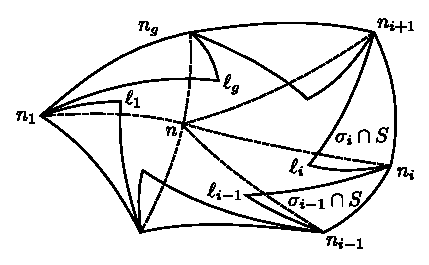
\includegraphics{vol58-fig/fig58-25.eps} 
\end{figure}

\end{prop}

\begin{proof}
If $Temb(\Delta)$ were projective, then Corollary \ref{chap1:coro6.5}, there exists
$a_i,\break b_i \in \mathbb{Z}$ and $m_i = m(\sigma_i)\in M$ for $1 \le i \le
g$ such that. 
$$
\langle m_i,\ell_i \rangle = -a_i, \langle m_i, n_i \rangle = -b_i, 
\langle m_i,n_{i+1} \rangle = -b_{i+1} 
$$
and  
$$
\langle m_{i-1}, \ell_i\rangle >  -a_i, \langle m_{i-1}, n_{i+1}\rangle >
-b_{i+1}, 
$$
for $1\le i\le g$, where $m_0 = m_g$. We see immediately that 
$0<\langle m_{i-1}$, $\ell_i \rangle +a_i= -\alpha_{i+1}\{\langle
m_{i-1},n_{i+1}\rangle +b_{i+1} \} + \gamma_i \{\langle
m_{i-1},n\rangle - \langle m_i,n\rangle \}$, hence  
$$
\langle m_{i-1},n\rangle > \langle m_i,n\rangle \qquad 1\le i\le g, 
$$
a contradiction.
\end{proof}

Let $\{n, n', n''\}$\pageoriginale be a $\mathbb{Z}$-basis of $N$, and
let $\ell = -(n + n' + n'')$. Let $P$ be the surface of the
tetrahedron in $N_{\mathbb{R}}$ with vertices $n$, $n'$, $n''$, $\ell$, which has
0 as the bary center. For $0 \neq y\in N_{\mathbb{R}}$, let us call
$(\mathbb{R}_\circ y)\cap P$
the point $y$ on $P$. For $d\ge 7$, consider the following subdivision 
$P_d$ of $P$, where the bottom triangle $nn'n''$ is left as it is.  
\begin{equation*}
\left. 
\begin{aligned}
n_1 & = n,n_2 = n', \; n_3 = n''\\
n_4 & = \ell\\
n_5 & = n_3 + n_4\\
n_6 & = n_1 + n_4\\
n_j & = n_6 + (j-6)n_4 ~(6 \le j \le d-1)\\
n_d & = n_2 + n_4
\end{aligned}
 \right\}
\end{equation*}

\begin{figure}[H]
\centering 
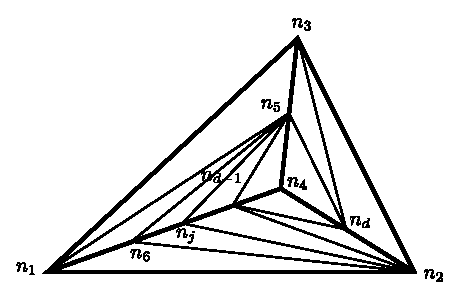
\includegraphics{vol58-fig/fig58-26.eps} 
\end{figure}

\begin{prop}\label{chap1:prop9.4}%%% 9.4
For $d \ge 7$, let $\Delta_d$ be the f.r.p.p.decomposition of $N_R$
obtained by joining $0$ with the simplices of the above subdivision
$p_d$. Then we have the following: 
\begin{enumerate}[(i)]
\item $X_d=Temb (\Delta_d)$ is a non-projective complete non-singular
  3 - dimensional tours embedding. 

\item There exists a $T$-equivariant surjective morphism from $X_d$ to
  $\mathbb{P}_3$. 

\item $X_d$ cannot be (not necessarily equivariantly) blown down along
  any non-singular center. 

\item The tours embedding obtained by blowing up $X_d$ along the curve
  $\overline{orb(\mathbb{R}_on_3+ \mathbb{R}_on_d)}$ is projective,
  and is obtained from $\mathbb{P}_3$ by\pageoriginale a succession of
  blowing ups along $T$-stable curves.  
\end{enumerate}
\end{prop}

\begin{proof}
It is immediate to see that $X_d$ is complete and non-singular. $X_d$
is non-projective by proposition \ref{chap1:prop9.3} applied to the polygon
$nn'n''n$ of $\underset{\sigma\epsilon\Delta_d}{\bigcup}(\sigma\cap
S)$, with $(\mathbb{R}_o\ell)\cap S$  to be taken as $n$ in Proposition 9.3
$(ii)$ is obvious, since $P_d$ is a subdivision of $P$. $(iii)$ If
$X_d$ were obtained by blowing up a non-singular variety along a
non-singular center, then the exceptional divisors is automatically
$T$-stable. But it is easy to check that $X_d$ cannot be equivariantly
blown along a non-singular center. $(iv)$ is immediate.  
\end{proof}

\begin{remark*}
The case $d=7$ is the simplest non-projective complete non-singular
3-dimensional torus embedding, which was already described in in
Miyake-Oda \cite{keyMO}. See the next  page for the picture of $T$-orbits
under the process described in $(iv)$ Demazure \cite[Appendice]{keyD2}
previously gave an example of non projective complete non-singular
3-dimensional torus embeddings which has 32 $T$-stable irreducible
divisors instead of 7 in our case. We latter get many other
non-projective examples as the by-products of our partial
classification below.
\newpage

\pageoriginale
\begin{figure}[H]
\centering 
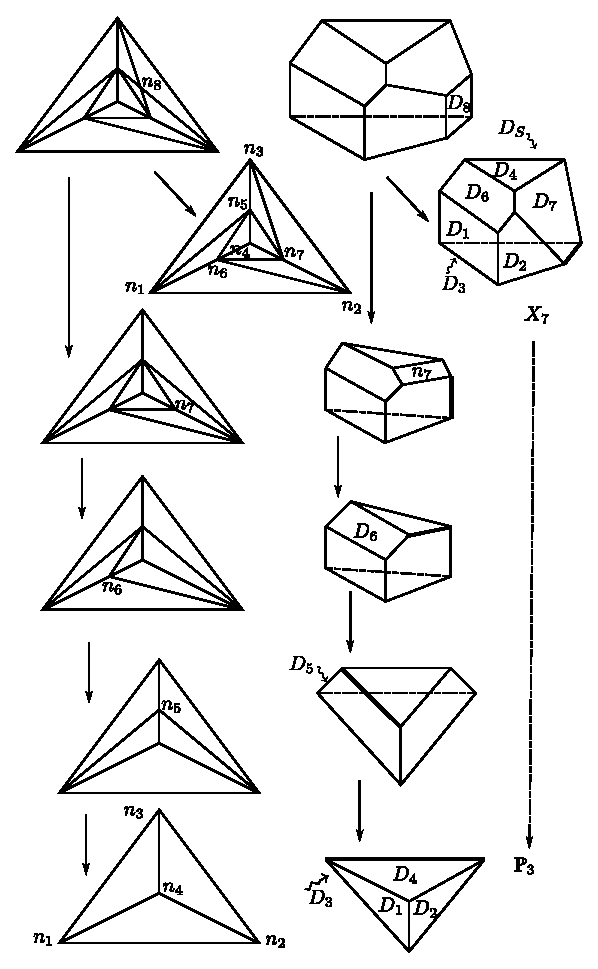
\includegraphics{vol58-fig/fig58-27.eps} 
\end{figure}
\end{remark*}
 
By analogy,\pageoriginale consider instead the 3-dimensional cone 
$$
\sigma = \mathbb{R}_on + \mathbb{R}_n' + \mathbb{R}_on''
$$
and let $\ell' = n + n' + n''$. For $d \ge 7$, let $\Delta'_{d}$ be
the subdivision of $\sigma$ which looks like this: 
\begin{figure}[H]
\centering 
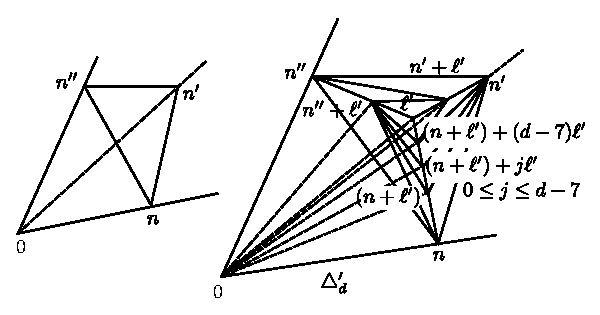
\includegraphics{vol58-fig/fig58-28.eps} 
\end{figure}

Then the following example gives as answer to a question raised by
Fujiki. 

\setcounter{coro}{4}
\begin{coro}\label{chap1:coro9.5}% Coro 9.5
The equivariant proper morphism
$$
f : Y_d = Temb(\Delta'_{d}) \to U(\sigma) = k^3
$$
is non-projective and cannot be written as a succession of blowing ups
along non-singular centers. But the blowing up $Y'_{d}$ of $Y_d$ along
$$\overline{orb(\mathbb{R}_on'' + \mathbb{R}_o(n' + \ell'))}$$ 
is obtained first by blowing up $U(\sigma)$ along the T-fixed point and
then by successively blowing up along $T$-stable curves.  
\end{coro} 

\begin{proof}% proof
All except the non-projectivity of $f$ are immediate. Consider the
tetrahedron with vertices $n$, $n'$, $n''$ and $\ell = -(n + n' + n'')$, and
its subdivision which $\Delta'_{d}$ induces on the face $nn'n''$. By
Proposition \ref{chap1:prop9.3}, we have a surjective morphism from a
non-projective 
complete non-singular torus\pageoriginale embedding to
$\mathbb{P}_3$. Since $f$ is obviously its restriction to
$U(\sigma)\subset\mathbb{P}_3$, we are done.  
\end{proof}

It is possible to describe projective equivariant birational morphism
directly in terms of the corresponding subdivision. We refer the
reader to Mumford et al. \cite[Chap. III, p. 152-154 in
  particular]{keyTE}. See also Namikawa \cite{keyN6}. 

\begin{remark*}
On the other hand, we can show in a similar fashion that the following
subdivision $\Delta^{''}_{d}$  of $\sigma = \mathbb{R}_on +
\mathbb{R}_on' + \mathbb{R}_on''$ 
gives rise to a {\em{projective}} morphism $Temb
(\Delta^{''}_{d})\to U(\sigma)\cong k^3$ which cannot be written as a
finite succession of blowing ups along non-singular centers, but can
be if $Temb(\Delta^{''}_{d})$ is blown up once  along
$\overline{\orb(\mathbb{R}_on' + \mathbb{R}_o(3n + n' + 2n''))}$. 
\begin{figure}[H]
\centering 
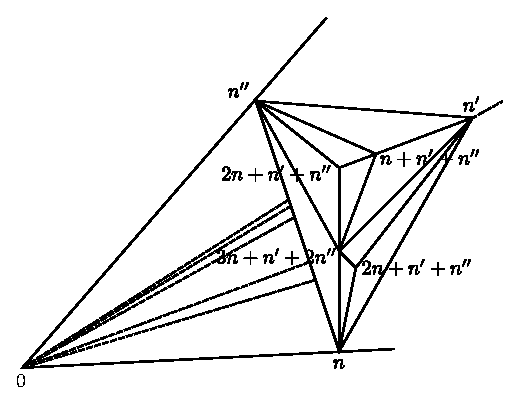
\includegraphics{vol58-fig/fig58-29.eps} 
\end{figure}

\end{remark*}

Let\pageoriginale $d$ be the number of spherical vertices of a
triangulation of $S^2$. Then obviously we have  
\begin{align*}
3d-6 & = \text{ the number of spherical edges }\\
\quad 2d-4 & = \text{ the number of spherical triangles}.\tag{*}
\end{align*}

\noindent
If the triangulation is of form $ S = 
\underset{\sigma\epsilon\Delta}{\cup}(\sigma \cap S)$ with $ X =
Temb(\Delta)$ complete non-singular, then $d$ = the cardinality of
$Sk^1(\Delta)$, $3d - 6 = $ the number of 2-dimensional cones in
$\Delta, 2d -4 =$ the number of 3-dimensional cones in $\Delta$. By
Proposition \ref{chap1:prop6.1}, we have  
$$
d-3=\text{ the Picard number of }X. 
$$ 

Furthermore for $v\ge 3$, let $p_v$ be the number of $v$-valent 
spherical vertices of a triangulation of $S^2$. Then we see that  
\begin{equation*}
\sum_{v\ge 3}(6-v)p_v=12.\tag{**} 
\end{equation*}

By Proposition \ref{chap1:prop9.1}, the classification of complete non-singular
3-dimensional torus embedding is reduced to 
\begin{enumerate}[(i)]
\item the classification of combinatorially different triangulations
  of $S^2$ and  

\item the different admissible $N$-weightings (or admissible double
  $\mathbb{Z}-weightings$) on them. 
\end{enumerate}

According to Gr\"unbaum \cite[Chap.13]{keyG3} \cite{keyG4}, we have the following
relevant facts: By Steinitz's theorem (which is known to be false in
higher dimension) the combinatorial equivalence classes of the
triangulation of $S^2$ are in one to one correspondence with the
combinatorial types of convex simplicial polyhedral in $\mathbb{R}^3$. Given
$d$, there seems, however, to be no formula for the number of
the\pageoriginale latter. It is empirically known for smaller values
of $d$ as follows: 
\begin{center}
\begin{tabular}{c|c|c|c|c|c|c|c|c|c|}
d & 4 & 5 & 6 & 7 & 8 & 9 & 10 & 11 & 12\\
\hline
& 1 & 1 & 2 & 5 & 14 & 50 & 233 & 1249 & 7595
\end{tabular} 
\end{center}
 
 \noindent
 In this connection, Eberhard's theorem \cite[13.3]{keyG3} looks
 intriguingly relevant to us, in view of our description of blowing
 ups along non-singular centers immediately before Corollary \ref{chap1:coro9.2}. 
 
 Anyway for $d\le 8$, we have the list in the next page of the
 combinatorially different triangulation of $S^2$, where we
 stereographically project them onto the plane from one of the
 spherical vertices, and we express circular arcs on the plane simply
 be liner arcs. 
 
 Among 7595 different triangulation for $d = 12$, we have the one
 induced by an icosahedron. 

For the classification of complete non-singular 3-dimensional torus
embeddings, it remains to find possible admissible $N$-weightings on
them. Obviously, it is enough to find those \textit{without any
  vertices which can be eliminated by blowing downs along non-singular
  centers}. 

\noindent
Combinatorial\pageoriginale types of the triangulation of $S^2$ for $d
\le 8$  
\begin{figure}[H]
\centering 
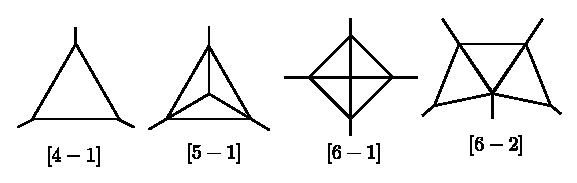
\includegraphics{vol58-fig/fig58-30.eps} 
\end{figure}
%%%
\begin{figure}[H]
\centering 
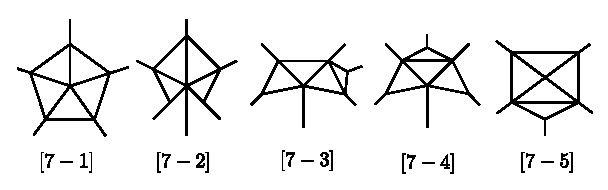
\includegraphics{vol58-fig/fig58-31.eps} 
\end{figure}
%%%
\begin{figure}[H]
\centering 
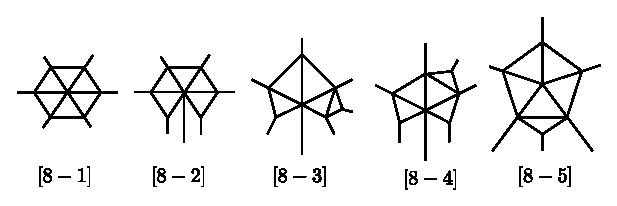
\includegraphics{vol58-fig/fig58-32.eps} 
\end{figure}
%%%
\begin{figure}[H]
\centering 
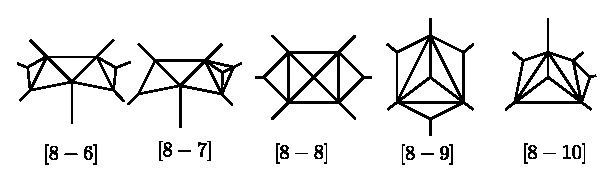
\includegraphics{vol58-fig/fig58-33.eps} 
\end{figure}
%%%
\begin{figure}[H]
\centering 
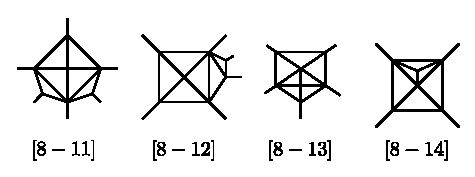
\includegraphics{vol58-fig/fig58-34.eps} 
\end{figure}
Icosahedron.
\begin{figure}[H]
\centering 
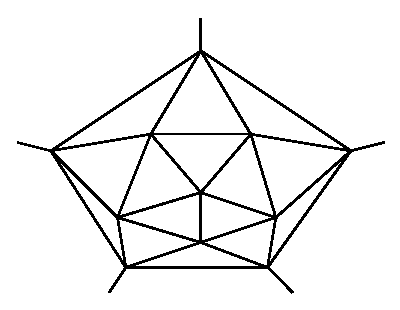
\includegraphics{vol58-fig/fig58-35.eps} 
\end{figure}

\setcounter{theorem}{5}
\begin{theorem}\label{chap1:thm9.6}
Let $X$\pageoriginale be a 3-dimensional complete non-singular torus
embedding which \textit{cannot be blown down along any no-singular
  center}. Then $X$ is isomorphic to one among the projective space
$\mathbb{P}_3$  
$$
\mathbb{P}_2-\text{bundles over } \mathbb{P}_1 \qquad
\mathbb{P}(0_{\mathbb{P}_1} \oplus 0_{\mathbb{P}_1} (a) \oplus
0_{\mathbb{P}_1} (b))\quad a, b \in \mathbb{Z}
$$
$\mathbb{P}_1$-bundles
$\mathbb{P}(0_Y \oplus L)$ over complete non-singular 2-dimensional
torus embeddings $Y$ and $L \in Pic(Y)$ and, if the Picard number $d-3
\leq 5$, Temb$(\triangle)$ corresponding to the following 13
different sequences with integral parameters of admissible
$N$-weighted triangulations of $S^2$, where $\{n,  n', n''\}$ is a
$\mathbb{Z}$-basis of $N=\mathbb{Z}^3$. 
%\end{theorem.}
\begin{figure}[H]
\centering 
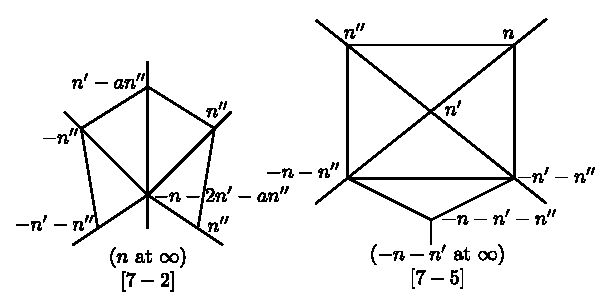
\includegraphics{vol58-fig/fig58-36.eps} 
\end{figure}
%%%
\begin{figure}[H]
\centering 
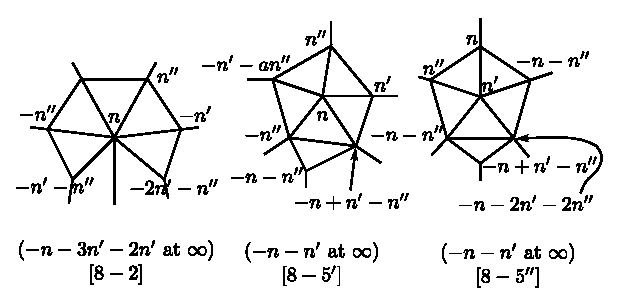
\includegraphics{vol58-fig/fig58-37.eps} 
\end{figure}
%%%
\pageoriginale
\begin{figure}[H]
\centering 
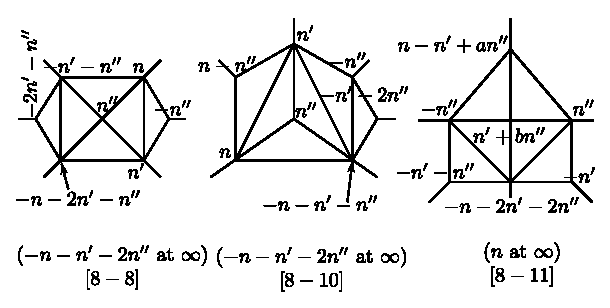
\includegraphics{vol58-fig/fig58-38.eps} 
\end{figure}
%%%
\begin{figure}[H]
\centering 
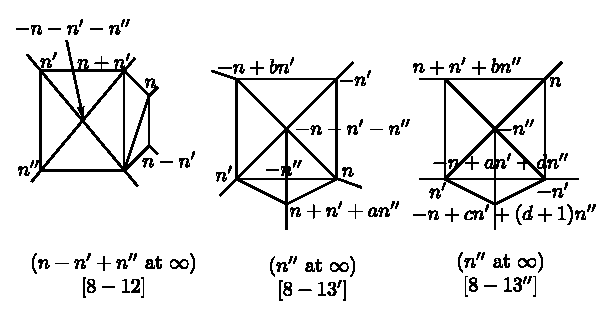
\includegraphics{vol58-fig/fig58-39.eps} 
\end{figure}
%%
\begin{figure}[H]
\centering 
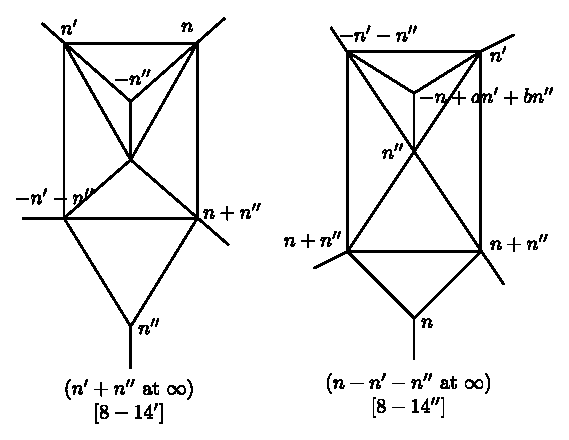
\includegraphics{vol58-fig/fig58-40.eps} 
\end{figure}

\end{theorem}

\begin{remark*} 
This\pageoriginale theorem was already announced in Miyake-Oda \cite{keyMO}
except that [8-12] was not counted there. This fact, as well as the
considerable simplification of the proof below, was pointed out by
Nagaya \cite{keyN2}.  
\end{remark*}

\begin{remark*}
Some of the torus embeddings listed in Theorem \ref{chap1:thm9.6} can
be blown down 
along a non-singular center if the integral parameters take special
values. $\mathbb{P}_3$, $\mathbb{P}_2$-bundles,
$\mathbb{P}_1$-bundles, [7-2], [8-2] and [8-10] are all
projective. On the other hand, [7-5] and $[8-5'']$ are $X_7$ and
$X_8$ of Proposition \ref{chap1:prop9.4}, respectively, hence are
non-projective. We 
can show that $[8-5'] (a \neq 0)$,  [8-8], [8-12], $[8-14']$ and
$[8-14'']$ are non-projective, using Proposition
\ref{chap1:prop9.3}. $[8-13']$ and 
$[8-13'']$ are not projective, except when they can be blown down for
special values of the integral parameters. For these torus embeddings
we can easily check the weak version of the conjecture at the
beginning of this section. 
\end{remark*}

	For simplicity, we adopt the following definition. 

	\begin{defi*}
 An admissible $N$-weighted triangulation of
 $S^2$ is called\break \textit{weakly minimal} if the corresponding
 complete non-singular center, i.e. the $N$-weighted
 triangulation has no 3-valent or 4-valent vertex which
 can be eliminated by blowing down along any non-singular
 center. 
	\end{defi*}

\setcounter{proofofthm}{5}	
\begin{proofofthm} %proof of Theorem 9.6
If $d=4$,\pageoriginale then $X \cong \mathbb{P}_3$ as a special case
of Theorem \ref{chap1:thm7.1}. in the remainder of the proof, we repeatedly use
Corollary \ref{chap1:coro9.2}, without explicit reference, to determine admissible
$N$-weightings or the corresponding double $\mathbb{Z}$-weightings for
a given triangulation of $S^2$ with $d \geq 5$. The argument depends
very much on the distribution of the valency of the vertices.  
\end{proofofthm}

\setcounter{lemma}{6}
\begin{lemma}\label{chap1:lem9.7}
For $d \geq 5$, let $[d-1]$ be the triangulation of $S^2$ which looks
like the picture. A weakly minimal admissible $N$-weighting on it is
necessarily of the following form up to isomorphism and corresponds to
a projective torus embedding: 

\begin{figure}[H]
\centering 
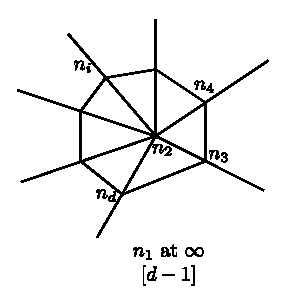
\includegraphics{vol58-fig/fig58-41.eps} 
\end{figure}


\begin{enumerate}[(1)]
 \item $d=5$, and $\{n_3, n_4, n_5\}$ are collinear. In this case, the
   corresponding torus embedding is a $\mathbb{P}_2$-bundle over
   $\mathbb{P}_1$. 

 \item $d \geq 5 $, $n_1 + n_2=0$ and $\{n_1, n_i, n_2 \}$ are
   collinear for all $3 \leq i \leq d $. In this case, the
   corresponding torus embedding is a $\mathbb{P}_1$-bundle over a
   $2$-dimensional complete non-singular torus embedding determined by
   the images of $n_i, 3 \leq i \leq d$, in $N/\mathbb{Z}n_1$. 
 \end{enumerate}
 \end{lemma}

 \begin{proof}
If $d = 5$, look at the 4-valent vertices $n_3$, $n_4$, $n_5$. Then by
Corollary \ref{chap1:coro9.2}, either $\{n_3, n_4, n_5\}$ are collinear hence on a
great circle, or $\{ n_1, n_i, n_2\}$ are collinear for all $3
\leqslant i \leq 5$. Thus we easily get (1) or (2) $d=5$ by
\ref{chap1:subsec7.6'}$'$. 
 \end{proof} 

 	If $d=6$,\pageoriginale the triangulation is symmetric with
        respect to the 
        pairs $\{n_1, n_2\}, \{n_3, n_5\}$, and $\{n_4, n_6\}$. Again
        by Corollary \ref{chap1:coro9.2} applied to the 4-valent vertices, we may
        assume that $n_1$ and $n_2$ are antipodal,
        i.e. $n_1+n_2=0$. Hence we get (2) $d=6$, by \ref{chap1:subsec7.6'}$'$  

 \noindent
 When $d \geq 7$, look at the $4$-valent vertices $n_3, \dots,
 n_d$. If $\{n_1, n_i, n_2\}$ were collinear for at most one $3 \leq i
 \leq d$, then $\{n_3, n_4, \dots , n_d\}$ would be on a great circle
 by Corollary \ref{chap1:coro9.2}. Since the valency of $n_2$ is $d-2 \geq 5$, the
 weighted link of $n_2$ would have weight $-1$ at some $n_j, 3
 \leqslant j \leqslant d$, which could be eliminated by blowing
 down. If $\{n_1, n_i, n_2\}$ were collinear for exactly two $i's$,
 $i=3$ and $j$ say, then $\{n_1, n_3, n_2, n_j\}$ would be on a great
 circle, and $\{n_3, n_4, \ldots , n_j\}$ and $\{n_j, n_{j+1}, \ldots,
 n_d\}$ would be collinear. Since $n_3$ and $n_j$ would then be
 antipodal, and since $\{n_3, n_2, n_j\}$ would be collinear, the
 weighted link of $n_2$ would have weight $-1$ at some $n_i, i \neq 3,
 j$, which could again be eliminated. Thus we conclude that $\{n_1,
 n_i, n_2\}$ are collinear for more than two, hence for all $3 \leq i
 \leq d$, since $n_1$ and $n_2$ are necessarily antipodal. In view of
\ref{chap1:subsec7.6'}$'$  again, we are done.  

 \begin{lemma}\label{chap1:lem9.8}
For $d \geq 6$, let $[d-2]$ be the triangulation of $S^2$ which looks
like the picture below. A weakly minimal admissible $N$-weighting on it
satisfies the following conditions: 
$\{n_3, n_4, \ldots , n_d\}$\pageoriginale are collinear, $n_1,
n_2=n_3 + n_d$. There exists $4 \leq j \leq d -3$, such that
$\{n_j, n_1, n_{j+2}\}$ and $\{n_j, n_2, n_{j+2}\}$ are collinear.   

\begin{figure}[H]
\centering 
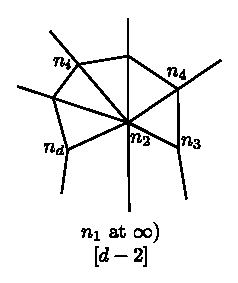
\includegraphics{vol58-fig/fig58-42.eps} 
\end{figure}
The corresponding torus embeddings are always projective.
 
\noindent
In particular, we have $d \geq 7$, and the only possible weakly
minimal admissible N-weightings for $d=7, 8$ are [7-2] 
and [8-2] in Theorem \ref{chap1:thm9.6} up to isomorphism.
\end{lemma}

\begin{proof}
If $d=6$, look at the weighted link of the 5-valent vertex
$n_2$. Its weight at $n_3$ and $n_6$ cannot be $-1$, since otherwise
$n_3$ or $n_6$ can be eliminated. Thus $\{n_3, n_2, n_6 \}, \{n_1,
n_4, n_2\}$ and $\{n_1, n_5, n_2\}$ are collinear again by Corollary
\ref{chap1:coro9.2}. This means that $n_1$ and $n_2$ are antipodal, a
contradiction 
to the strong convexity of cones. 

Let $d \geq 7$. Since $n_1$ and $n_2$ cannot be antipodal, there can
be at most one $4 \leq i \leq d- 1$ such that $\{ n_1, n_i, n_2\}$ are
collinear, hence on a great circle. If there were one such $i$, the
weighted link of $n_2$ would have weight $-1$ at some $n_j, 3 \leq j
\leq d,  j \neq i$, but $\{ n_3, n_4, \ldots, n_i\}$ and $\{n_i,
n_{i+1}, \ldots , n_d\}$ would be collinear, a contradiction. Thus we
conclude that $\{n_3, n_4, \ldots , n_d\}$ are collinear. Now look at
the weighted link of $n_1$ $(resp. n_2)$. Then weight $-1$ is possible
only at $n_2$ $(resp. n_1)$.\pageoriginale Thus $n_1 +  n_2=n_3 +n_d$,
and together 
with $n_3, \ldots , n_d$ it lies on a great circle. Moreover, $\{ n_j,
n_1, n_{j+2}\}$ and $\{ n_j, n_2, n_{j+2}\}$ are collinear for some $4
\leq j \leq d- 1$. If $d= 7$ or $8$, there is only one possible such
weighted link. The projectivity of the corresponding torus embeddings
follows easily from Corollary \ref{chap1:coro9.5} in view of the projectivity of
$2$-dimensional torus embeddings (Proposition \ref{chap1:prop8.1}) and
the fact that 
$n_1 + n_2 =n_3 +n_d, n_3 \ldots , n_d$ are on a great circle. 
\end{proof}


\begin{lemma}[Nagaya]\label{chap1:lem9.9}
 For $d \geq 7$, the triangulation $[d-3]$ below has no weakly
  minimal admissible $N$-weightings. 
\end{lemma}

\begin{proof}
Suppose there were a weakly minimal admissible $N$-weighting. Since
$n_1$ and $n_2$ cannot be antipodal, there is at most one $5 \leq j
\leq d -1$ such that $\{n_1, n_j, n_2\}$ are collinear, hence on a
great circle. 
\begin{figure}[H]
\centering 
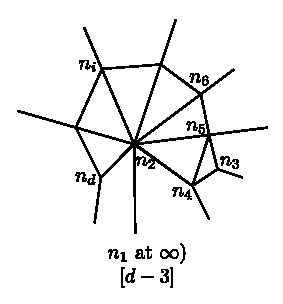
\includegraphics{vol58-fig/fig58-43.eps} 
\end{figure}

If there were one such $j$, look at the $4$-valent
vertex $n_4$. $\{n_1, n_4, n_5\}$ could not be collinear, since
otherwise they would be on a great circle disjoint from the great
circle above. Hence $\{n_2, n_4, n_3\}$ would be collinear. Then look
at the weighted link of $n_5$. The weight $-1$ could not be at $n_3$
nor $n_4$. If $\{n_1, n_5, n_4\}$ were collinear, then they would be
on a great circle disjoint from another great\pageoriginale circle, a
contradiction. Thus $\{n_2, n_5, n_3\}$ would be collinear, hence
$n_2, n_3$ are antipodal, a contradiction again. We thus conclude that
$\{n_1, n_i, n_2 \}$ are not collinear for all $5 \leq i \leq d-1$,
hence $\{n_5, n_6, \ldots , n_d\}$ are collinear. Look at the vertex
$n_4$ again. If $\{n_1, n_4, n_5 \}$ were collinear, the $\mathbb{Z}$-
weight of the edge $n_2n_4$ at $n_4$ would coincide with that of
$n_3n_4$ at $n_4$, which is $1$. Then look at the weighted link of
$n_2$. There would exist $6 \leq j \leq d$ such that $\{n_4, n_2,
n_j\}$ are collinear. Thus it has weight $-1$ at some $n_k, 6 \leq k
\leq d$, $k \neq j$, 4, 1, 5, a contradiction. 

Thus $\{n_2, n_4, n_3\}$ are collinear. Look at the weighted link of
$n_5$. Since it cannot have weight $-1$ at $n_3$ and $n_4$, either
$(i) \{n_1, n_5, n_4\}$ are collinear, i.e. on a great circle, hence
$\{n_4, n_1, n_5 \}$ are collinear, or (ii) $\{n_2, n_5, n_3\}$ are
collinear, hence $n_2, n_3$ are antipodal, and $\{n_2, n_1, n_3\}$ are
collinear. In both cases, the weighted link of $n_1$ would have weight
$-1$ at some $n_k, 6 \leq k \leq d$, a contradiction, since $\{n_5,
n_6, \ldots, n_d\}$ are collinear. 
\end{proof}

\begin{lemma}[Nagaya]\label{chap1:lem9.10}
 For $d \geq 7$, the triangulation $[d-4]$ below has no weakly
  minimal admissible $N$-weighting. 
\end{lemma}

\begin{proof}
Suppose the contrary. Since the weighted link of $n_5$ cannot have
weight $-1$ at $n_3$ and $n_4$, $\{n_3, n_5, n_4\}$ are
collinear.\pageoriginale Look at the weighted link of $n_6$. Since its
weight at $n_3$ cannot be $-1$, we have three possibilities:  
\begin{figure}[H]
\centering 
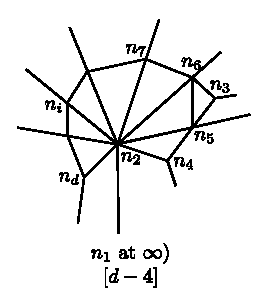
\includegraphics[scale=0.7]{vol58-fig/fig58-44.eps} 
\end{figure}

  \begin{enumerate}[(i)]
 \item $\{n_1, n_6, n_5\}$ are collinear, hence on a great
   circle. Since $\{n_1, n_5, n_6\}$ are then collinear, the weighted
   link of $n_5$ has weight $-1$ at $n_4$, a contradiction. 
 \item $\{n_3, n_6, n_7\}$ are collinear. In this case, the weighted
   link of $n_5$ and the $\mathbb{Z}$-weights around $n_5$ can be
   determined completely by means of the compatibility in Corollary
   \ref{chap1:coro9.2}. We see easily that the weighted link of $n_1$ has positive
   weights at $n_4$ and $n_5$, a contradiction. 

 \item $\{n_2, n_6, n_3\}$ are collinear. Again using the
   compatibility of the $\mathbb{Z}$-weights around $n_5$, we easily
   see that $\{n_4, n_2, n_6\}$ are collinear, hence $n_3$ and $n_4$
   are antipodal. Thus $\{n_3, n_1, n_4\}$ are also collinear. Since
   $n_2, n_2$ cannot be antipodal, $\{n_1, n_i, n_2\}$ can be
   collinear for at most one $5 \leqslant i \leqslant d-1$. Suppose
   $\{n_l, n_j, n_2\}$ were collinear, hence on a great circle. If
   $j=5$, then $n_3$ could be eliminated. If $6 \leqslant j$, then a
   pair $n_3, n_4$ of antipodal points would lie strictly on one side
   of the great circle, a contradiction. Thus $\{n_1, n_i, n_2\}$ are
   not collinear for any $5 \leq i \leq d -1$, hence $\{ n_6, n_7,
   \ldots , n_d\}$ are  
 collinear.\pageoriginale Look at the weighted link of $n_2$. Since
 $\{n_4, n_2,  n_6\}$ are assumed to be collinear, there exists $7
 \leq k \leq d$  such that its weight at $n_k$ is $-1$, a
 contradiction.  
 \end{enumerate}
 \end{proof}

  \begin{lemma}[Nagaya]\label{chap1:lem9.11}
 For $d \geq 8$, the triangulation $[d-6]$ below has no weakly
    minimal admissible $N$-weighting. 
  \end{lemma}

\begin{proof}
Suppose the contrary. Since $n_1$, $n_2$ cannot be antipodal, $\{n_1,
n_i,\break n_2\}$ can be collinear for at most one $6 \leq i \leq d -1$. 
\begin{figure}[H]
\centering 
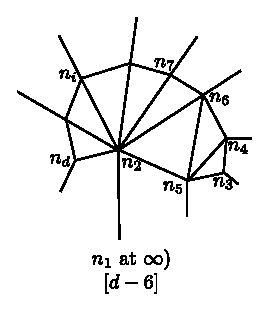
\includegraphics[scale=0.75]{vol58-fig/fig58-45.eps} 
\end{figure}
\begin{enumerate}[(1)]
\item Suppose for one $6 \leq j \leq d-1$, $\{n_1, n_j, n_2\}$ were
  collinear, hence on a great circle. Then $\{n_j, n_{j+1}, \ldots ,
  n_d\}$ are collinear. Since $\{n_1, n_2, n_j\}$ are collinear, the
  consideration of the weighted link of $n_2$ shows that $j=d-1$. Look
  at the weighted link of $n_4$. Since $\{n_1, n_4, n_5\}$ cannot be
  on a great circle, we see that $\{n_3, n_4, n_6\}$ are
  collinear. Look then at the weighted link of $n_5$. From what we
  have seen so far, we can conclude that $\{n_3, n_5, n_6\}$ are
  collinear, hence $n_3, n_6$ are antipodal and are strictly on one
  side of the great circle passing through $n_1, n_2, n_{d-1}$, a
  contradiction. 

\item We thus conclude that $\{n_1, n_i, n_2\}$ are not collinear for
  all $6 \leq i \leq d-1$, hence $\{n_6, n_7, \ldots , n_d \}$ are
  collinear. 
\end{enumerate}
Look\pageoriginale at the weighted link of $n_4$.
\end{proof}

\noindent
(2-i) If $\{n_1, n_4, n_5\}$ are not collinear, then $\{n_3, n_4,
n_6\}$ are collinear. The weighted link of $n_5$ forces $\{n_3, n_5,
n_6\}$ to be collinear, hence $n_3, n_6$ are antipodal and $\{n_3,
n_1, n_6\}$ are collinear. Look at the weighted link of $n_1$ and
$n_2$ simultaneously. Their weights at $n_i, 7 \leq i \leq d$,
coincide. $(2-i-a)$ Suppose $\{n_j, n_2, n_k\}, 6 \leq j < k \leq d$,
were collinear. Since $n_3, n_4$ are antipodal, $n_2 n_j
n_{j+1}\ldots n_kn_2$ cannot be a great circle, hence $n_j, n_k$ are
antipodal. The sequence of weights of the weighted link of $n_2$ at
$n_{j+1}, \ldots , n_{k-1}$ is a part of that of the weighted link of
$n_1$ at $n_7$, $n_8, \ldots , n_d, n_1, n_5$. We easily see that this
is a contradiction. $(2-i-b)$ If $\{ n_1, n_2, n_j\}, 6 \leq j \leq
d$, are collinear, then $n_1 n_j n_2n_1$ is a great circle, which
determines a hemisphere containing a pair $n_3, n_6$ of antipodal
points, a contradiction. (2-i-c) Suppose $\{n_5, n_2, n_j\}, 6 \leq j
\leq d$, are collinear. Then the consideration of the weights at
$n_{j+1}, \ldots , n_d, n_1$ of the weighted link of $n_2$ show that
$j=d$. Look then at the weighs at $n_6, n_7, \ldots, n_{d-1}$ of the
weighted link of $n_2$. There would be $-1$ somewhere, a
contradiction. 

\noindent
$(2-ii)$ Suppose $\{n_1, n_4, n_5\}$ are collinear, hence on a great
circle and $\{ n_4, n_1, n_5 \}$ are collinear. Look at the weighted link of
$n_1$ and $n_2$. As in $(2-i)$, we arrive at a contradiction. 

\begin{lemma}[Nagaya]\label{chap1:lem9.12}
 For\pageoriginale $d \geq 8$, the triangulation $[d-7]$ has no weakly
  minimal admissible $N$-weighting. 
\end{lemma}

\begin{proof}
Suppose the contrary. Again $\{n_1, n_i, n_2\}$ can be collinear for
at most one $6 \leq i \leq d-1$. 
\begin{figure}[H]
\centering 
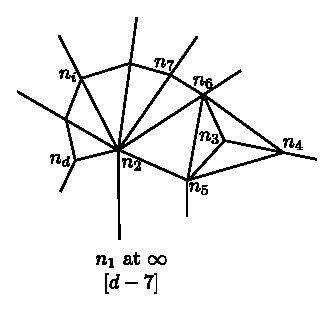
\includegraphics{vol58-fig/fig58-46.eps} 
\end{figure}
\begin{enumerate}[(1)]
\item Suppose $\{n_1, n_j, n_2\}$, $6 \leq j \leq d-1$, are collinear,
  hence on a great circle. Hence $\{n_1, n_2, n_j\}$, $\{n_6, n_7,
  \ldots , n_j\}$ and 
  $\{n_j, n_{j+1}, \ldots , n_d\}$ are collinear. Looking at the
  weighted link of $n_2$, we again see that $j = d-1$, $\{n_6, \ldots ,
  n_{d-1}\}$ are collinear and $n_1 n_2 n_{d-1} n_1$ is a great
  circle. Look then at the weighted link of $n_4$. Obviously, $\{ n_5,
  n_4, n_6\}$ are not collinear, hence $\{ n_1, n_4, n_3\}$ are
  collinear and $\{n_4, n_5, n_6\}$ are not. At 5-valent $n_5, \{ n_1,
  n_5, n_3\}$ are necessarily collinear, but we have a contradiction,
  since then $n_1, n_3$ are antipodal and $n_1n_2n_{d-1}n_1$ is a
  great circle. 

\item We conclude that $\{ n_1, n_i, n_2\}$ are not collinear for all
  $6 \leq i \leq d -1$, hence $\{n_6, n_7, \cdots , n_d\}$ are
  collinear. Look at the weighted link of $n_4$. 
\end{enumerate}

\noindent
$(2-i)$ If $\{ n_5, n_4, n_6\}$ are collinear, hence on a great
circle,  the compatibility of the $\mathbb{Z}$-weights around
$5$-valent $n_5$ shows that the weighted link of $n_2$ has a positive
weight at $n_5$. 

\noindent
$(2-ii)$\pageoriginale If $\{ n_5, n_4, n_6 \}$ are not collinear,
then $\{ n_1, 
n_4, n_3 \}$ are collinear. At 5-valent $n_5$, we see that $\{
n_1, n_5, n_3 \}$ are collinear, hence $n_1, n_3$ are antipodal and
$\{ n_1, n_6, n_3 \}$ are collinear, Again by  the compatibility of
the $\mathbb{Z}$ weights around $n_5$, we see that the weighted link
of $n_2$ has a positive weight at $n_5$. 

In both cases $(2-i)$ and $(2-ii)$, look at the weighted link of
$n_2$. Since it has a positive weight ar $n_5$, $\{ n_5, n_2, n_k \}$
are collinear for some $7 \le k \le d$, hence has weight $-1$ at
some $n_1$, $6 \le i \le d$, $i \neq k$, a contradiction. 
\end{proof}

\begin{lemma}\label{chap1:lem9.13}
A weakly minimal admissible $N$-weighting for the triangulation
[7-5] is necessarily of the form in Theorem \ref{chap1:thm9.6} up to
isomorphism. 
\end{lemma}

\begin{proof}
By symmetry, we may assume that $\{ n_3, n_1, n_6 \}$ are
collinear.\break Look at the weighted link of $n_2$. 
\begin{figure}[H]
\centering 
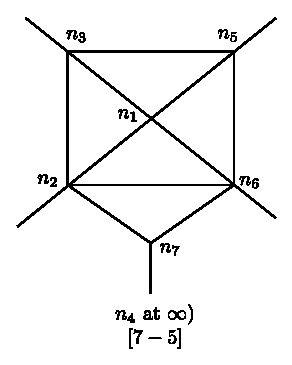
\includegraphics[scale=0.8]{vol58-fig/fig58-47.eps} 
\end{figure}

Since the weights at
$n_1$ and $n_7$ cannot be $-1$, $\{ n_1, n_2, n_7 \}$ are necessarily
collinear. Since its weight at $n_3$ is then $-1$, $\{ n_2, n_3, n_5
\}$ are collinear. Thus $\{ n_3, n_4, n_7 \}$ and $\{ n_1, n_5, n_4
\}$ are collinear for the same reason. Looking then at the weighted
link of $n_6$ , we see that $\{ n_5, n_6, n_7 \}$ are collinear. From
what we have seen so far, an admissible double $\mathbb{Z}$ weighting
is uniquely determined as in the picture, by Cor.9.2.
\begin{figure}[H]
\centering 
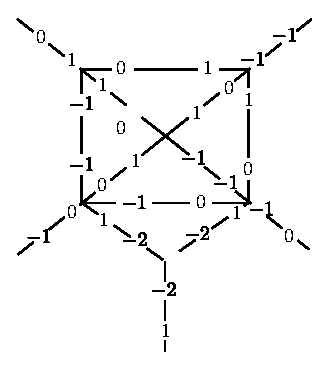
\includegraphics[scale=0.8]{vol58-fig/fig58-48.eps} 
\end{figure}\pageoriginale
 $n = n_5$, $n'= n_1$, $n''= n_3$ form a $\mathbb{Z}$-basis of
$N$. The double $\mathbb{Z}$ weighting successively determines the
other $N$-weights as follows: $n_2 = -n n''$, $n_4 = -n -n'$, $n_6 =
-n' -n''$ and $n_7 = -n -n''$.  
\end{proof}

\begin{lemma}\label{chap1:lem9.14}
A weakly minimal admissible $N$-weighting on the triangulation [8-5]
is either [$8-5'$] or [$8-5''$] of Theorem \ref{chap1:thm9.6} up to isomorphism. 
\end{lemma}

\begin{proof}
Neither $\{ n_1, n_4, n_2 \}$ nor $\{ n_1, n_8, n_2 \}$ are collinear,
since otherwise the $\mathbb{Z}$ weights around $n_3$ would be
$-1$. 
\begin{figure}[H]
\centering 
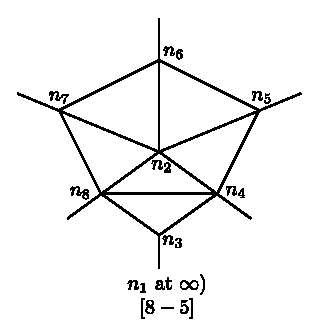
\includegraphics[scale=0.8]{vol58-fig/fig58-49.eps} 
\end{figure}

In particular, $n_1, n_2$ are not antipodal. Thus $\{ n_1, n_i,
n_2 \}$ are collinear for at most one $5 \le i \le 7$. If there were
no such i, then $n_4n_5n_6n_7n_8n_4$ would necessarily be a great
circle and the weighted link of $n_4$ would have weight $-1$ at $n_3$,
a contradiction. By symmetry, it thus suffices to consider the 
following two cases: 
\begin{enumerate}
\item $\{ n_1, n_5, n_2 \}$ are collinear, hence $\{ n_5, n_6, n_7,
  n_8 \}$ are collinear. Look at the weighted link of $n_4$. We easily
  see that $\{ n_3, n_4, n_5 \}$ are collinear. Look then at the
  weighted link\pageoriginale of $n_2$. If $\{ n_5, n_2, n_7 \}$ were
  collinear, then 
  $n_5n_2n_7n_1n_5$ would be a great circle, thus $\{ n_2, n_7, n_1
  \}$ would be collinear, a contradiction. Thus we conclude that $\{
  n_6, n_2,\break n_8 \}$ are collinear. In particular, $n_6 , n_8$ are
  antipodal, hence $\{ n_6, n_1,\break n_8 \}$ are also collinear.  Then the
  weighted link of $n_1$ has necessarily weights $-2, -1, -2$ at $
  n_3, n_4, n_5 $, respectively.   Looking at the $\mathbb{Z}$
  weights around $n_4$ determined so far,  we see that the weighted
  link of $n_8$ has weight 0 at $n_4$, hence $\{ n_2, n_8, n_3 \}$
  are collinear.  The collinearity for each vertex thus determined
  gives rise to a unique admissible double $\mathbb{Z}$ weighting with
  one integral parameter, which determines the admissible
  $N$-weighting [$8-5'$] in Theorem \ref{chap1:thm9.6},  if we let  $n = n_2, n' =
  n_5  , n'' = n_6$. 

\item $\{ n_1, n_6, n_2 \}$,  hence $\{ n_4, n_5, n_6 \}$ and $\{ n_6,
  n_7, n_8 \}$  are collinear. Look at the weighted link of $n_2$. We
  see that $\{ n_5, n_2, n_7 \}$ are collinear. Look then at the
  weighted link of $n_4$ and $n_8$. By symmetry and because of the
  fact that their weights at $n_3$ cannot be $-1$, we have four
  possibilities: 
\end{enumerate} 
\end{proof}

\begin{enumerate}[(i)]
\item $\{ n_1, n_4, n_8 \}$ are collinear, hence are on a great
  circle. Look at the weighted link of $n_1$. Its weights at $ n_5,
  n_6, n_7$ are necessarily. $-2,\break -1, -2$. By the compatibility of the
  $\mathbb{Z}$ weights around the $4$-valent vertex $n_5$, we have a
  contradiction. 

\item $\{ n_2, n_4, n_3 \}$ and $\{ n_2, n_8, n_3 \}$ are collinear,
  hence $n_2, n_3$ are antipodal. We see then that $\{ n_3, n_1, n_6
  \}$ are collinear. Then\pageoriginale the weighted link of $n_1$
  leads us to a contradiction.  

\item $\{ n_3, n_4, n_5 \}$ and $\{ n_3, n_8, n_7 \}$ are collinear,
  hence $n_3, n_6$ are antipodal. Again we see that $\{ n_3, n_1, n_6
  \}$ are collinear, a contradiction. 

\item $\{ n_3, n_4, n_5 \}$ and $\{ n_3, n_8, n_2 \}$ are collinear.
  Then by the compatibility of the $\mathbb{Z}$weights around the
  vertices $n_7$ and $n_8$, we see that the weighted link of $n_1$ has
  weight $-3, -1, -2, -1, 1, 0$ at $n_3, n_4, n_5, n_6,\break n_7, n_8$,
  respectively, hence in particular $\{ n_3, n_1, n_7 \}$ are
  collinear.  An admissible double $\mathbb{Z}$ -weighting is uniquely
  determined by\break these considerations and gives rise to the admissible
  N-weighting [$8-5''$] of Thm \ref{chap1:thm9.6}. 
\end{enumerate}

\begin{lemma}\label{chap1:lem9.15}
A weakly minimal $N$-weighting on the triangulation [8-8] is of the
form in Theorem \ref{chap1:thm9.6} up to isomorphism.  
\end{lemma}

\begin{proof}
By symmetry, we may assume that $\{ n_4, n_1, n_5 \}$ are
collinear.\break Looking at the weighted link of $n_2$ and of $n_3$, we see
that $\{ n_1, n_2, n_6 \}$ and $\{ n_1, n_3, n_7 \}$ are
collinear.
\begin{figure}[H]
\centering 
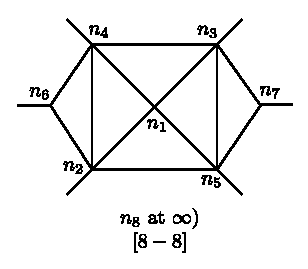
\includegraphics{vol58-fig/fig58-50.eps} 
\end{figure}


 Look then at the weighted link of $n_4$ and of $n_5$.  $\{
n_2, n_4, n_8 \}$ are not collinear, since otherwise they would be on
a great circle, hence a contradiction for the weighted link of $n_2$
would result. Similarly, we see that $\{ n_3, n_5, n_8 \}$ are not
collinear. By symmetry,  we thus have three possibilities: 
\begin{enumerate}
\item $\{ n_1, n_4, n_6 \}$\pageoriginale and $\{ n_1, n_5, n_7 \}$
  are collinear. Then $\{ n_1,  n_6 \}$ and $\{ n_1, n_7 \}$ are
  pairwise antipodal, a contradiction.  

\item $\{ n_3, n_4, n_6 \}$ and $\{ n_2, n_5, n_7 \}$ are collinear.
  Let the weighted link of $n_2$ have weight $b$ at $n_6$. The
  collinearity we have so far then determines all the
  $\mathbb{Z}$-weights around $n_2$ in terms of $b$. But the
  compatibility for them leads to $b = -1$, a contradiction. 

\item $\{ n_3, n_4, n_6 \}$ and $\{ n_1, n_5, n_7 \}$ are collinear.
  Let the weighted link of $n_2$ have weight $b$ at $n_6$. Then the
  compatibility of the $\mathbb{Z}$ weights around $n_2$ shows that
  $\{ n_5, n_8, n_6 \}$ are collinear.  Hence the weighted link of
  $n_8$ necessarily has weights $-2, -1$ at $n_7, n_3, n_4$,
  respectively.  In this way, an admissible double $\mathbb{Z}$
  -weighting is uniquely determined and gives rise to the admissible
  N-weighting [8-8] of Thm \ref{chap1:thm9.6}.  
\end{enumerate}
\end{proof}

\begin{lemma}\label{chap1:lem9.16}
The triangulation [8-9] has no weakly minimal admissible
$N$-weighting. 
\end{lemma}

\begin{proof}
Suppose the contrary. Look at the weighted link of $n_1$.  By
symmetry, it is enough to consider three cases. 
\begin{figure}[H]
\centering 
\includegraphics{vol58-fig/fig58-51.eps} 
\end{figure}

\begin{enumerate}
\item $\{ n_2, n_1, n_3 \}$ are collinear, hence on a great
  circle. Looking at the\pageoriginale weighted link of $n_2, n_3$ and
  $n_4$, we immediately get a contradiction.  

\item $\{ n_2, n_1, n_6 \}$ are collinear.  In this case,  the 
  weighted link of $n_1$ has weights $-1$ at $n_7$ and $n_8$, a
  contradiction. 

\item $\{ n_6, n_1, n_7 \}$ are collinear.  The same argument applies 
  to the other $6$ valent vertices $n_2, n_3$ and $n_4$.  But for the
  weighted link of $n_2$, $\{ n_5, n_2, n_8 \}$ cannot be collinear,
  since otherwise we would easily conclude that $\{ n_3, n_2, n_4 \}$
  are also collinear hence on a great circle,  a contradiction by
  $(1)$ applied to $n_5$ instead of $n_1$.  Taking into account the
  similar conclusion for $n_3$, we need, by symmetry,  to consider the
  following three cases: 
\end{enumerate}
\end{proof}

\begin{enumerate}[(i)]
\item $\{ n_5, n_2, n_7 \}$ and $\{ n_5, n_3, n_6 \}$ are collinear.
  In this case, the consideration of the weighted link of $n_2$ and
  $n_3$ leads us to a contraction for the weighted link of $n_1$  

\item $\{ n_5, n_2, n_7 \}$ and $\{ n_6, n_3, n_8 \}$ are collinear.

\item $\{ n_7, n_2, n_8 \}$ and $\{ n_6, n_3, n_8 \}$ are collinear.
\end{enumerate}

\noindent
In cases $(ii)$ and $(iii)$, the $\mathbb{Z}$- weights around $n_6,
n_7,n_8$ are necessarily $0, 0, -2$ a contradiction for the weighted
link of $n_1$. 

\begin{lemma}\label{chap1:lem9.17}
A weakly minimal admissible $N$-weighting for the triangulation [8-10]
is necessarily of the form in Theorem \ref{chap1:thm9.6} up to isomorphism. 
\end{lemma}

\begin{proof}
Note first that the triangulation can be written in a more symmetric 
form as on the right hand side. 
\begin{figure}[H]
\centering 
\includegraphics{vol58-fig/fig58-52.eps} 
\end{figure}\pageoriginale


Look at the weighted link of $n_1$. Then $\{ n_7, n_1, n_8 \}$. are
collinear.  Look then at the weighted link of $n_2$. Then $\{ n_3,
n_2, n_4 \}$ are not collinear, hence $\{ n_5, n_2, n_6 \}$ are
collinear. Indeed, if otherwise, $\{ n_3, n_2, n_4 \}$ would be a
great circle. Then looking at the weighted link of $n_3$ and $n_4$, we
would get a contradiction for the weighted link of $n_1$. 

If $\{ n_5, n_3, n_6 \}$ or $\{ n_5, n_4, n_6 \}$ were collinear, then
$n_5, n_6$ would be antipodal, and we would get a contradiction for
the weighted link of $n_1$. 

If $\{ n_2, n_3, n_4 \}$ or $\{ n_2, n_4, n_3 \}$ were collinear, then
they would be on a great circle, a contradiction again. 

Thus for the weighted link of $n_3$, either $\{ n_2, n_3, n_7 \}$ or
$\{ n_1, n_3, n_6 \}$ are collinear. We have a similar conclusion for
the weighted link of $n_4$. By symmetry, we need to consider the
following three cases: 
\begin{enumerate}
\item $\{ n_1, n_3, n_6 \}$\pageoriginale and $\{ n_1, n_4, n_6 \}$
  are collinear. We get a contradiction for the weighted link of
  $n_1$.    

\item $\{ n_2, n_3, n_7 \}$ and $\{ n_2, n_4, n_8 \}$ are collinear.
  In this case, we have a contradiction for the $\mathbb{Z}$-weights
  around $n_7, n_8$, and $n_2$. 

\item $\{ n_1, n_3, n_6 \}$ and $\{ n_2, n_4, n_8 \}$ are collinear.
  In this case, we can determine all the double $\mathbb{Z}$-weights
  uniquely from the collinearity conditions so far. We get the unique
  admissible N-weighting described in Theorem \ref{chap1:thm9.6}. 
\end{enumerate}
\end{proof}

\begin{lemma}\label{chap1:lem9.18}
A weakly minimal admissible $N$-weighting for the triangulation [8-11]
is of the form in Theorem \ref{chap1:thm9.6} up to isomorphism.  
\end{lemma}

\begin{proof}
Look at the weighted link of $n_1$ and $n_2$. By symmetry, we need to
consider the following three cases: 
\begin{figure}[H]
\centering 
\includegraphics{vol58-fig/fig58-53.eps} 
\end{figure}
\begin{enumerate}
\item $\{ n_4, n_1, n_2 \}$ and $\{ n_1, n_2, n_3 \}$ are collinear,
  hence $\{ n_1, n_2, n_3 , n_4 \}$ are on a great circle. We easily
  get a contradiction for the weighted link of $n_5$. 

\item $\{ n_4, n_1, n_2 \}$ and $\{ n_5, n_2, n_6 \}$ are collinear.
  In this case,  $n_1, n_5, n_7$ and $n_1, n_6, n_8$ are necessarily
  collinear.  The consideration of the weighted link of $n_3$ shows
  that\pageoriginale $\{ n_5, n_3, n_6 \}$  are collinear,   hence
  $n_5, n_6$ are antipodal.  

\item $\{ n_5, n_1, n_6 \}$ and $\{ n_5, n_2, n_6 \}$ are collinear,
  hence $n_5, n_6$ are again antipodal. 
\end{enumerate}
\end{proof}

Thus in cases (2) and (3), $n_5$ and $n_6$ are antipodal, hence
$\{ n_5, n_3, n_6 \}$ and $\{ n_5, n_4, n_6 \}$ are collinear.  Look
at the weighted link of $n_5$. Since $\{ n_3, n_5, n_4 \}$ cannot be
on a great circle,  and since the situation is symmetric with respect
to $n_3$ and $n_4$, we may assume that $\{ n_2, n_5, n_7 \}$ are
collinear. Looking at the weighted link of $n_4$ and the
$\mathbb{Z}$-weights around $n_7, n_8$ and $n_1$, we conclude that $\{
n_2, n_6, n_8 \}$ are collinear.  From what we have seen so far,  we
get a unique admissible double $\mathbb{Z}$-weighting with two
integral parameters, which gives rise to the admissible N-weighting
described in Theorem \ref{chap1:thm9.6}. 

\begin{lemma}[Nagaya]\label{chap1:lem9.19}
 A weakly minimal admissible $N$-weighting on the
  triangulation [8-12] is of the form in Theorem \ref{chap1:thm9.6} up to
  isomorphism. 
\end{lemma}

\begin{proof}
The triangulation can again be written in a more symmetric form as on
the right hand side.
\begin{figure}[H]
\centering 
\includegraphics[scale=0.75]{vol58-fig/fig58-54.eps} 
\end{figure}

By symmetry,  we may assume that $\{ n_3, n_1,
n_7 \}$ are collinear.\pageoriginale  Look at the weighted link of
$n_2$ and of $n_3$. We need to consider three cases:  
\begin{enumerate}
\item If $\{ n_3, n_2, n_7 \}$ are collinear,  then $n_3, n_7$ are
  antipodal, hence $\{ n_3, n_5,\break n_7 \}$ and $\{ n_3, n_6, n_7 \}$ are
  collinear.  Looking at the weighted link of $n_5$, we see that $\{
  n_5, n_4, n_8 \}$ are collinear,  a contradiction for the weighted
  link of $n_6$.  

\item If $\{ n_1, n_2, n_5 \}$ and $\{ n_1, n_3, n_5  \}$ are
  collinear,  then $n_1, n_5$ are antipodal, hence $\{ n_1, n_6, n_5
  \}$, $\{ n_1, n_7, n_5 \}$ and $\{ n_3, n_5, n_7 \}$ are collinear.
  Looking at the weighted link of $n_5$, we see that $\{ n_5, n_4, n_8
  \}$ are collinear, again a contradiction for the weighted link of
  $n_6$. 

\item Let $\{ n_1, n_2, n_5 \}$ and $\{ n_2, n_3, n_6 \}$ be
  collinear.  If $\{ n_6, n_4, n_7 \}$ were collinear hence on a great
  circle, the weighted link of $n_7$ would have weight $-2$ at
  $n_2$. Moreover, the weighted link of $n_5$ would have weight 1 at
  $n_4$, hence $\{ n_3, n_5, n_4 \}$ would be collinear and the weight
  at $n_2$ would be $-1$. Since the weighted link of $n_1$ has weight
  $0$ at $n_2$, we would violate the compatibility for the
  $\mathbb{Z}$-weights around $n_2$. 
\end{enumerate}
\end{proof}

Thus we conclude that $\{ n_3, n_1, n_7 \}$ , $\{ n_1, n_2, n_5 \}$,
$\{ n_2, n_3, n_6 \}$ and $\{n_5,\break n_4, n_8 \}$ are collinear.  We
then have three possibilities for the weighted link of $n_5$. If $\{
n_3, n_5, n_7 \}$ were collinear, then $n_3, n_7$ would be antipodal,
a contradiction, since we are in case (1). If $\{ n_2, n_5, n_6 \}$
were collinear, then $\{ n_1, n_2,  n_5, n_6 \}$ would be on a great
circle, hence $n_2, n_6$ would\pageoriginale be antipodal. By
symmetry, we are in case (1), a contradiction. Thus $\{ n_3, n_5, n_4
\}$ are collinear.  

We then four possibilities for the weighted link of $n_6$.  If $\{
n_3, n_6, n_4 \}$  were collinear, then $n_3, n_4$ would be antipodal,
hence $\{ n_1, n_7, n_4 \}$ would be collinear,  a contradiction for
the weighted link of $n_7$. If $\{ n_5, n_6, n_8 \}$ were collinear,
then $n_5, n_8$ would be antipodal, hence $\{ n_5, n_7, n_8 \}$ would
be collinear.  Looking at the weighted link of $n_6$ and $n_7$, we
would get a contradiction for the $\mathbb{Z}$- weights around $n_1$.
If $\{ n_4, n_6, n_7 \}$ were collinear hence on a great circle, $\{
n_4, n_7, n_6 \}$ would be collinear. Looking at the weighted link of
$n_6$ and $n_7$, we would again get a contradiction for the
$\mathbb{Z}$-weights around $n_1$. 

Thus $\{ n_1, n_6, n_8 \}$ are collinear. These collinearity
conditions determine a unique admissible double $\mathbb{Z}$-weighting,
which gives rise to the $N$-weighting [8-12] in Theorem 
\ref{chap1:thm9.6}.  

\begin{lemma}\label{chap1:lem9.20}
A weakly minimal admissible $N$-weighting on the triangulation [8-13]
is either [8-13] or [$8-13''$] of Theorem \ref{chap1:thm9.6} up to isomorphism. 
\begin{figure}[H]
\centering 
\includegraphics{vol58-fig/fig58-55.eps} 
\end{figure}
\end{lemma}

\begin{proof}
Look at\pageoriginale the weighted link of $n_1$ and $n_2$. By
symmetry, it suffices to consider three cases:  
\begin{enumerate}
\item $\{ n_2, n_1, n_6 \}$ and $\{ n_1, n_2, n_7 \}$ are
  collinear. Look at the weighted link of $n_5$. By symmetry, we may
  assume that $\{ n_2, n_5, n_6 \}$, hence $\{ n_4, n_3, n_5 \}$ are
  collinear.  Thus $n_2 , n_6$ are antipodal, and $\{ n_2, n_8, n_6
  \}$ are collinear.  Looking at the weighted link of $n_8$, we see
  that $\{ n_3, n_4, n_8 \}$ are collinear. We have two possibilities
  for the weigh\-ted link of $n_6$, but by symmetry with respect to $\{
  n_3, n_4 \}$, we may assume that $\{ n_3, n_6, n_8 \}$ are
  collinear.  Thus $n_3 , n_8$ are antipodal, hence $\{ n_3, n_7, n_8
  \}$ are collinear.  These collinearity conditions determine a unique
  admissible double $\mathbb{Z}$ -weighting with two integral
  parameter which gives rise to the N-weighting [$8-13'$] of Theorem
\ref{chap1:thm9.6}.  

\item $\{ n_5, n_1, n_8 \}$ and $\{ n_5, n_2, n_8 \}$ are collinear.
  In this case $n_5, n_8$ are antipodal, hence $\{ n_5, n_6, n_8 \}$
  and $\{ n_5, n_7, n_8 \}$ are collinear.  Looking at the weighted
  link of $n_6$ and $n_7$, we see that $\{ n_6, n_3, n_7 \}$ and $\{
  n_6, n_4, n_7 \}$ are collinear, hence $n_6, n_7$ are antipodal and
  $\{ n_6, n_5, n_7 \}$ and $\{ n_6, n_8, n_7 \}$ are collinear.
  These collinearity conditions determine a unique admissible double
  $\mathbb{Z}$-weighting with four integral parameters, which gives
  rise to the $N$-weighting [$8-13''$] of Theorem \ref{chap1:thm9.6}. 

It remains to show that the following cannot happen:

\item $\{ n_5, n_1, n_8 \}$ and $\{ n_1, n_2, n_7 \}$ are collinear. 
\end{enumerate}  
\end{proof}

\noindent
By symmetry with respect to $\{ n_3, n_4 \}$ and our argument (1),
(2) applied\pageoriginale to $n_3, n_4$ instead of $n_1, n_2$, we may
assume that $\{n_6, 
n_3, n_7\}$ and $\{n_3, n_4, n_8\}$ are collinear. Looking at the
weighted link of $n_5$ and $n_6$, we see then that $\{n_2, n_5, n_3\}$
and $\{n_1, n_6, n_4\}$ are collinear. Let a (resp $b$) be the
$\mathbb{Z}$-weight of the edge $n_3n_5$ at $n_3$ (resp. $n_1n_6$ at
$n_1$). Then the $\mathbb{Z}$-weights around 4-valent vertices $n_1,
n_2, n_3, n_4$ are determined in terms of $a$ and $b$. We see that
$a, b\neq 0, -1$. Looking at the compatibility of the
$\mathbb{Z}$-weights around $n_7$ and $n_8$, we see that $\{n_4, n_7,
n_5\}$ and $\{n_2, n_8, n_6\}$ are collinear. Then we have $a(b+1)=
b(a+1)=-1 ,a $ contradiction, since $a\neq -1$ and $b\neq -1$. 

\begin{lemma}\label{chap1:lem9.21}
A weakly minimal admissible $N$-weighting on the triangulation [8-14]
is either [$8-14'$] or [$8-14''$] of Theorem \ref{chap1:thm9.6} up to
isomorphism.  
\end{lemma}

\begin{proof}
The triangulation can be written in a more symmetric from again. 
\begin{figure}[H]
\centering 
\includegraphics[scale=0.75]{vol58-fig/fig58-56.eps} 
\end{figure}

First\pageoriginale  look at the 5-valent $n_3$, $n_4$, $n_5$ around
$n_1$ (1). If $\{n_3, 
n_4, n_5\}$ are collinear, then they are on a great circle. Look at
the weighted link of $n_6$. Because of the 3-valent vertex $n_2,
\{n_5, n_6, n_8\}$ and $\{n_4, n_6, n_7\}$ are not collinear $\{n_7,
n_6, n_8\}$ are not collinear, since otherwise they would be on a
great circle disjoint from the other great circle $n_3, n_4, n_5,
n_3$. Thus by  symmetry we may assume that $\{n_2, n_6, n_5 \}$ are
collinear. Look at the weighted link of $n_7$. If $\{n_2, n_7, n_5 \}$
were collinear, then $n_2, n_5$ would be antipodal, a contradiction,
since $n_2$ is not on the great circle $n_3 n_4 n_5 n_3$. For the same
reason as above, we thus conclude that $\{n_2, n_7, n_3\}$ and $\{n_2,
n_8, n_4\}$ are collinear. These collinearity condition determine a
unique admissible double $\mathbb{Z}$-weighting with two integral
parameters, which gives rise to the $N$-weighting [$8-14''$] of Theorem
\ref{chap1:thm9.6}.  

(2) By (1) and the symmetry around $n_1$, we need to consider two
cases: 

(i) $\{n_1, n_3, n_8\}, \{n_1, n_4, n_8\} \text{ and }\{n_1, n_5,
n_6\}$ are collinear. Let $b$ be the $\mathbb{Z}$-weight around
$n_1$. Then the weighted link of $n_3$ is completely determined in
terms of $b$. 

By the compatibility of the $\mathbb{Z}$-weights around $n_3$, the
weighted link of $n_8$ has weight $0$ at $n_3$, hence $\{n_4, n_8,
n_7\}$ are collinear, a contradiction. 

(ii) $\{n_1, n_3, n_7\}$,\pageoriginale $\{n_1, n_4, n_8\}$ and  $\{n_1, n_5,
n_6\}$ are collinear. Again let $b$ be the $\mathbb{Z}$-weighted
around $n_1$. The collinearity condition so far determine some the the
double $\mathbb{Z}-weights$. By our argument (1) applied to $n_2$
instead of $n_1$, we conclude easily that $\{n_2, n_8, n_4\}$, 
$\{n_2,n_6, n_5\}$ and $\{n_2, n_7, n_3\}$ are collinear. We thus get a
unique admissible double $\mathbb{Z}$-weighting with an integral
parameter,  which gives to the $N$-weighting [$8-14'$] of Theorem
\ref{chap1:thm9.6}. 
\end{proof}

We thus conclude the proof of Theorem \ref{chap1:thm9.6}.

\begin{remark*}
By repeated application of Corollary 9.2 we determined all
admissible $N$-weightings on the \textit{icosahedral} triangulation of
$S^2$. Apparently, there are 32 different admissible $N$-weightings,
some of which integral parameters, as in the table below, although
some of them might be redundant because of the symmetric nature of the
triangulation. 
\begin{figure}[H]
\centering 
\includegraphics{vol58-fig/fig58-57.eps} 
\end{figure}

Some of them are projective and some others are not. The weak version
of our conjecture  at the beginning of this section holds for all of
them. 

Since all the vertices are 5-valent, these admissible $N$-weightings are
automatically weakly minimal. In the table below let $\{n,n'n''\}$ be
a $\mathbb{Z}$-basis of $N$ and $a,b,c,d\epsilon,\mathbb{Z}$ 
\end{remark*}

\newpage

\pageoriginale
\rotatebox{90}{%
{\fontsize{9}{11}\selectfont
\begin{tabular}{rlllll}
&(1) & (2) & (3) & (4) & (5)\\[13pt]
$n_1$ & $-n+bn'+cn''$ & $-n'+bn''$ & $n-n'+an''$ & $-n+(a+1)n'+bn''$ &
  $n-an'-n''$\\[5pt] 
$n_2$ & $-n'+an''$ & $-n+an'+cn''$ & $-n'$ & $n'$ & $n$  \\[5pt] 
$n_3$ & $-n''$ & $n''$ & $n''$ & $-n''$ & $n'$\\[5pt] 
$n_4$ & $n'-n''$ & $n$ & $n$ & $-n+an'+cn'' $& $n'-n''$\\[5pt] 
$n_5$ & $n'$ & $n-n''$ & $n-n''$ & $-n+an'+(c+1)n''$ & $-n''$\\[5pt] 
$n_6$ & $n''$ & $-n''$ & $-n''$ & $n''$ & $-n'$\\[5pt] 
$n_7$ & $n-n'$ & $n+n'$ & $n+n'$ & $-n'$ & $-n+n'+bn''$\\[5pt] 
$n_8$ & $n$ & $n+n-n''$ & $n'$ & $-n'+n''$ & $-n$\\[5pt] 
$n_9$ & $n-n'+n''$ & $n'-n''$ & $-n'+bn'+cn''$ & $n$ & $cn-n'+n''$\\[5pt] 
$n_{10}$ & $n-2n'+an''$ & $-n+(a+1)n'+cn''$ & $-n+(b+1)n'(c+1)n''$ &
  $n-n-n''$ & $n''$\\[5pt]  
$n_{11}$ & $n-n'-n''$ & $n'n''$ & $n'+n''$ & $-n'-n''$ &
  $-n+n'+(b+1)n''$\\[5pt]  
$n_{12}$ & $n-n'$ & $n'$ & $2n'+n''$ & $n-n'$ & $-n+n''$
\end{tabular}}}


\pageoriginale
\rotatebox{90}{%
{\fontsize{9}{11}\selectfont
\begin{tabular}{rllll}
& (6) & (7) & (8) & (9)\\[15pt]
$n_1$ & $-n+bn'+cn''$ & $-n'+bn'+cn''$ & $-n+bn+an''$ & $n'-n''$\\[6pt]
$n_2$ & $n'$ & $n''$ & $n'-n''$ & $-n+bn'+(c-1)n''$\\[6pt]
$n_3$ & $n''$ & $-n''$ & $-n+bn'+(c+1)n''$ &  $n'$\\[6pt]
$n_4$ & $-n+(b-1)n'+(a+c)n''$ & $-n+bn'+(c-1)n''$ & $-n'+(a+1)n''$ &
  $n$\\[6pt] 
$n_5$ & $-n'+(a-1)n''$ & $n'-n''$ & $-n'+n''$ & $n-n''$\\[6pt]
$n_6$ & $-n''$ & $n'$ & $-n''$ & $-n''$\\[6pt]
$n_7$ & $n'+an''$ & $-n''$ & $n-n'+an''$ & $n-n'+an''$\\[6pt]
$n_8$ & $n-2n''$ & $n-n''$ & $n-n'$ & $-n'+an''$\\[6pt] 
$n_9$ & $n+n'-n''$ & $n$ & $-n'+n'+n''$ & $n+(b-1)n'+(a+c)n''$\\[6pt]
$n_{10}$ & $n$ & $n-n'+(a+1)n''$ & $n'$ & $-n+bn'+cn''$\\[6pt]
$n_{11}$ & $-n'+(a+1)n''$ & $-n'-n''$ & $n''$ & $n''$ \\[6pt]
$n_{12}$ & $n-n''$ & $n-n'+an''$ & $n$ & $-n+(a+1)n''$
\end{tabular}}}

\pageoriginale
\rotatebox{90}{%
{\fontsize{9}{11}\selectfont
\begin{tabular}{rlllll}
&(10) & (11) & (12) & (13) & (14)\\[15pt]
$n_1$ & $n-n'+an''$ & $an-n'-(b+1)n''$ & $an-n'-n''$ & $-n+an'+bn''$ &
  $n-n'+an''$\\[5pt] 
$n_2$ & $-n'+(a+1)n''$ & $-n-bn''$ & $n-n'$ & $-n+(b+1)n''$ & $n$\\[5pt] 
$n_3$  & $n$ & $n$ & $-n$ & $n'$ & $n''$\\[5pt] 
$n_4$ &$n-n''$ & $n-n''$ & $-n''$ & $n'-n''$ & $-n'$\\[5pt] 
$n_5$ &$-n''$ & $-n''$ & $n-n''$ & $-n''$ & $-n'-n''$\\[5pt] 
$n_6$ &$-n'+an''$ & $-n$ & $n$  & $-n'$ & $-n''$\\[5pt] 
$n_7$ & $n'-n''$ & $n'-n''$ & $n'-n''$ & $n$  & $-n$\\[5pt] 
$n_8$ &$-n+bn'+cn''$ & $-n+n'+bn''$ & $n'$ & $n-n'(b+1)n''$ & $-n-n''$\\[5pt] 
$n_9$ & $-n+bn'+(c+1)n''$ & $-n+n'(b+1)n''$ & $n'+n''$ & $n-n'-bn''$ &
  $-n+n'-n''$\\[5pt] 
$n_{10}$ & $n''$ & $n''$ & $n''$ & $n''$  & $n'$\\[5pt] 
$n_{11}$ & $n'$ & $n'$ & $-n+n'+bn''$ & $n+n'$ & $-n+bn'n''$ \\[5pt] 
$n_{12}$ &$-n+(b+1)n'+cn''$ & $-n+2n+bn''$ & $-n+2n'+bn''$ & $n+n''$ &
  $-n+n'$ 
\end{tabular}}}


\pageoriginale
\rotatebox{90}{%
{\fontsize{9}{11}\selectfont
\begin{tabular}{rlllll}
&(15) & (16) & (17) & (18) & (19)\\[15pt]
$n_1$ & $n-n'+an''$ & $n+n'an''$ & $n+n'+an''$ & $n+n'+an''$ & $n$\\[5pt]
$n_2$ & $n$ & $n$ & $n'$ & $n$ & $n-n'-(a-1)n''$\\[5pt]
$n_3$ & $-n''$ & $n''$ & $n''$ & $n''$ & $n''$\\[5pt]
$n_4$ & $-n'-n''$ & $n'+n''$ & $n+n''$ & $n'+n''$ & $n+n'-n''$\\[5pt]
$n_5$ & $-n'$ & $n'$ & $n$ & $n'$ & $-n'-2n''$\\[5pt]
$n_6$ & $n''$ & $-n''$ & $-n''$ & $-n''$ & $-n''$\\[5pt]
$n_7$ & $-n-n'-n''$ & $-n+bn'$ & $-n'$ & $-n$ & $n'-n''$\\[5pt]
$n_8$ & $-n$ & $-n-n''$ & $-n'-n''$ & $-n-n''$ & $-n+bn'+(a-1)n''$\\[5pt]
$n_9$ & $n+n'+n''$ & $n-n'$ & $-n+bn'-n''$ & $n-n'-n''$ & $-n'$\\[5pt]
$n_{10}$ & $n'$ & $-n'+n''$ & $-n$ & $-n'$ & $-n+(a+1)n''$\\[5pt]
$n_{11}$ & $-n-n''$ & $-n+bn'+n''$ & $-n-n'$ & $-n+n''+b(n'+n'')$ & $n'$\\[5pt]
$n_{12}$ & $-n+n'+b(n+n'+n')$ & $-n'$ & $-n+(b-1)n'-n''$ & $-n'-n''$ & 
$-n+bn'+an''$
\end{tabular}}}


\pageoriginale
\rotatebox{90}{%
{\fontsize{9}{11}\selectfont
\begin{tabular}{rllllll}
&(20) & (21) & (22) & (23) & (24) & (25)\\[15pt]
$n_1$ & $-n'+an''$ & $n''$ & $n$ & $n$ & $n+n'+an''$ & $-n+an'+(b+1)n''$\\[5pt]
$n_2$ & $-n-2n'$ & $-n-n'+(a+1)n''$ & $-n-n+an''$ & $-n-n'+(a+1)n''$ &
  $n+n''$ &  $-n+an'+bn''+c(n'-n'')$\\[5pt] 
$n_3$ & $n''$ & $-n'$ & $-n''$ & $-n''$ & $-n''$ & $n'-n''$\\[5pt]
$n_4$ & $n+n''$ & $n-n'-an''$ & $n+n'$ & $n+n'$ & $n+2n'+an''$ & $n'$\\[5pt]
$n_5$ & $n$ & $n$ & $n'+n''$ & $n'+n''$ & $n'+n''$ & $n''$\\[5pt]
$n_6$ & $-n''$ & $n'$ & $n''$ & $n''$ & $n''$ & $-n'+n''$\\[5pt]
$n_7$ & $2n+n'+n''$ & $-n''$ & $n'$ & $n'$ & $n'$ & $n$\\[5pt]
$n_8$ & $n+n'$ & $n+n'-n''$ & $-n+n'+an''$ & $-n+n'+an''$ & $-n$ &
  $n-n'+(d+1)n''$\\[5pt] 
$n_9$ & $n'-n''$ & $2n'-n''$ & $-n+an''$ & $-n+an''$ & $-2n-n'$ & $-n'$\\[5pt]
$n_{10}$ & $-n-n'$ & $-n+an''$ & $n'-n''$ & $n'-2n''$ & $-n-n'$ & $-n''$\\[5pt]
$n_{11}$ & $n'$ & $-n+(a-1)n''$ & $n+2n'-n''$ & $n+2n'-n''$ & $n'-n''$
  & $n-n''$\\[5pt]
$n_{12}$ & $-n+n'-n''$ & $n'-n''$ & $2n-n''$ & $n'-n''$ & $-n+n'-n''$
  & $n-n+dn''$
\end{tabular}}}

\pageoriginale
\rotatebox{90}{%
{\fontsize{9}{11}\selectfont
\begin{tabular}{rlllllll}
&(26) & (27) & (28) & (29) & (30) & (31) & (32)\\[15pt]
$n_1$ & $-n+an'+bn''$ & $-n+2n''$ & $n'-n''$ & $n'+2n''$ & $n-n'+2n''$
  & $3n'-n''$  & $n-n'-n''$\\[5pt] 
$n_2$ & $-n'+cn''$ & $-n-n'+n''$ & $-n-n''$ & $-n+2n''$ & $2n+n''$ &
  $-n+n'+2n''$ & $n-n'$\\[5pt] 
$n_3$ & $-n+an'+(b+1)n''$ & $-n'$ & $n'$ & $n'+n''$ & $-n+n''$ &
  $2n'-n''$ & $n$\\[5pt] 
$n_4$ & $n'$ & $n-n'-n''$ &  $n-n''$ & $n$ & $n''$ & $n-n'$ & $n-n''$\\[5pt]
$n_5$ & $n'-n''$ & $n''$ & $n-2n''$ & $n+n''$ & $n+2n''$ & $n$ &
  $n-n'-2n''$\\[5pt] 
$n_6$ & $-n''$ & $n'$ & $-n'$ & $n''$ & $n+n''$ & $n'$ & $-n'-n''$ \\[5pt]
$n_7$ & $n$ & $2n-n'$ & $-n'+2n''$ & $-n-n'n''$ & $n'+2n''$ &
  $-n-n'+n''$ & $n+n'-n''$\\[5pt] 
$n_8$ & $n-n''$ & $n$ & $-n'+n''$ & $-n'+n''$ & $n'+n''$ & $n+n''$ & $n'$\\[5pt]
$n_9$ & $n-n'+dn''$ & $2n'-n''$ & $-n$ & $-n-n'+n''$ & $n'$ & $n''$ &
  $-n-n'-n''$\\[5pt] 
$n_{10}$ & $-n'+(c+1)n''$ & $-n$ & $n'+n''$ & $-n+n''$ & $n$ & $-n+2n''$
  & $n+n''$\\[5pt] 
$n_{11}$ & $n''$ & $-n''$ & $n$ & $n'$ & $-n-n''$ & $n'-n''$ &
  $2n+n'-n''$\\[5pt]  
$n_{12}$ & $n-n'+(d+1)n''$ & $-n+n'-n''$ & $-n+n''$ & $-n-n'$ &
  $-n-n'-n''$ &  $ -n-n'+2n''$ & $n''$ 
\end{tabular}}}

